\documentclass[lang=cn,11pt]{elegantbook}

\title{大学物理（下）}
\author{夏同}
\institute{华南理工大学}
\date{\today}
\version{0.2}

\setcounter{tocdepth}{3}

\logo{logo-blue.png}
\cover{cover.jpg}

\usepackage{array}
\usepackage{amsmath,amssymb,mathtools}
\usepackage{siunitx}
\usepackage{physics}
\usepackage{tikz}
\usepackage{graphicx}
\makeatletter
\@ifundefined{newCJKfontfamily}{
  \providecommand{\physicskaishu}{\kaishu}
}{
  \newCJKfontfamily\physicskaishu[AutoFakeBold=2]{KaiTi}
}
\@ifundefined{citshape}{
  \newcommand{\citshape}{\physicskaishu}
}{
  \renewcommand{\citshape}{\physicskaishu}
}
\makeatother
\ExplSyntaxOn
\msg_redirect_name:nnn { siunitx } { physics-pkg } { none }
\ExplSyntaxOff

\newcommand{\bridge}[1]{\begin{note}#1\end{note}}
\newcommand{\chapterroadmap}[3]{%
\begin{introduction}
 \item {\heiti 这章解决什么问题：}#1
 \item {\heiti 你已经会什么：}#2
 \item {\heiti 这章新增什么：}#3
\end{introduction}}
\newcommand{\summaryline}[1]{\par\noindent\textbf{1分钟回顾：}#1\par}
\newcommand{\chapterselfcheck}[1]{\par\noindent\textbf{自测问题：}#1\par}

\begin{document}

\maketitle
\frontmatter
\pagenumbering{arabic}

\tableofcontents
\makeenvindex
\mainmatter

\chapter{真空中的静电场}

奥斯特发现，通有电流的导线附近，能够使小磁针发生偏转。这说明电流周围存在磁场。以前人们认为电现象属于电；磁现象属于磁；二者是互不相关的两类现象。但奥斯特的实验表明运动的电荷（电流），可以产生磁场。法拉第进一步思考：既然电流能产生磁场，那么磁场能不能反过来产生电流？经过大量实验，法拉第在 1831 年发现了电磁感应定律：当穿过闭合回路的磁通量发生变化时，回路中会产生感应电动势；如果回路闭合，就会产生感应电流。例如：
\begin{itemize}
\item 把磁铁插入线圈，线圈中产生电流；
\item 把磁铁从线圈中拔出，线圈中也产生电流；
\item 磁铁静止在线圈旁边，则通常没有感应电流；
\item 线圈面积、方向或磁场强度发生变化，也能产生感应电流。
\end{itemize}
所以，法拉第揭示了电现象和磁现象之间的另一种联系：变化的磁场能够产生电场。麦克斯韦在此基础上，把电学和磁学统一起来，建立了著名的麦克斯韦方程组。麦克斯韦方程组可以概括为四条规律：
\begin{itemize}
\item 电荷是电场的源；
\item 磁单极子不存在，磁力线总是闭合的；
\item 变化的磁场产生电场；
\item 电流和变化的电场产生磁场。
\end{itemize}
其中第四条是麦克斯韦的重要补充。也就是说，即使没有真实电荷在运动，只要电场随时间变化，也可以产生磁场。由这四条规律可以推出变化的电场产生磁场，变化的磁场又产生电场。这样，电场和磁场就可以相互激发、相互传播，形成电磁波。麦克斯韦进一步计算出电磁波的传播速度，发现这个速度正好等于光速。因此他提出光本身就是一种电磁波。这说明光、电、磁原来是统一的。后来赫兹通过实验验证了电磁波的存在。

\begin{definition}[场]
\begin{enumerate}
\item 场是一种物质存在形式：物质不只包括我们能直接看见、摸到的物体。物理学中，物质还可以以场的形式存在。例如一块带电的物体周围存在电场；一块磁铁周围存在磁场；地球周围存在引力场和地磁场；无线电台周围存在传播出去的电磁场。
\item 场是时空的函数：场的数值通常会随着位置和时间变化。电场可以写成：\(\mathbf E=\mathbf E(\mathbf r,t)\)，磁场可以写成：\(\mathbf B=\mathbf B(\mathbf r,t)\)。其中\(\mathbf r\) 表示空间位置；\(t\) 表示时间；\(\mathbf E\) 和 \(\mathbf B\) 不仅有大小，还有方向，因此是矢量场。例如，点电荷周围的电场，离电荷越近，电场越强；离得越远，电场越弱，而且不同位置的电场方向也不同。
\end{enumerate}
\end{definition}

\begin{theorem}[电磁场的几个基本特征]
\begin{enumerate}
  \item 场无处不在，并且可以延伸到整个空间：这里的“无处不在”不能简单理解为“每一个位置的场都很强”，而是说只要有场源，场原则上就会存在于它周围的空间中。例如，地球的引力场和地磁场会延伸到很远的地方。一个带电体产生的电场，也不会突然在某个位置截断。理想情况下，点电荷的电场可以延伸到无限远：
\[
E=\frac{1}{4\pi\varepsilon_0}\frac{|q|}{r^2}
\]但是，电场强度会随着距离 \(r\) 增大而按 \(1/r^2\) 减小。
实际测量中，当距离足够远时，场会小到仪器测不出来，所以我们通常可以忽略它。
\item 场的作用范围可以很大，但影响传播速度有限：场的影响通常会随着距离减弱。例如离电荷越远，电场越弱；离电流越远，磁场越弱；离无线发射源越远，接收到的信号通常越弱。
\item 场的作用范围可以很大，但影响传播速度有限。在实际问题中，我们经常可以采用近似方法。比如研究一根导线附近的磁场时，如果某个很远的物体受到的磁场作用小得可以忽略，就不需要把它纳入计算。不过还需要补充一点：电磁作用的变化并不是瞬间传遍整个空间。电磁场的变化以有限速度传播，真空中的最大传播速度就是光速：\(c\approx 3.0\times10^8\ \text{m/s}
\)因此，电磁作用不是传统意义上的“超距作用”，而是通过场在空间中逐步传播。
\item 物体之间的相互作用要通过场来传递。如果电荷的位置发生变化，这种变化会先改变附近的电场，然后电磁场的变化再以光速传播到远方。因此，远处的电荷不会在同一时刻立即知道近处发生了什么。
\item 机械波通常需要介质。例如声波需要空气或其他介质；水波需要水；绳上的波需要绳子。但是电磁波不需要物质介质，它可以在真空中传播。太阳光经过真空到达地球，就是一个典型例子。
\end{enumerate}
\end{theorem}

\begin{figure}[htbp]
\centering

\includegraphics[width=0.4\textwidth]{pdf-exercises/21.png}
\caption{电场磁场示意图}
\end{figure}

平面电磁波中电场方向；磁场方向，波的传播方向，三者互相垂直。如果电磁波沿 \(x\) 方向传播，电场沿 \(y\) 方向振动，那么磁场就沿 \(z\) 方向振动。可以写成：
\[
\mathbf E\perp\mathbf B,~~~~
\mathbf E\perp\text{传播方向},\qquad
\mathbf B\perp\text{传播方向}
\]因此，电磁波是横波。图中红色和蓝色波形的波峰、波谷相互对应，表示它们随时间和空间同步变化。在真空中的平面电磁波中，电场和磁场同相：电场达到最大值时，磁场也达到最大值；电场为零时，磁场也为零。二者的大小关系为\(E=cB\)，其中 \(c\) 是真空中的光速。

\section{电荷}

\begin{definition}[电荷的量子化]
  电荷不是可以任意连续取值的，而是以一个最基本的电荷量 \(e\) 为单位，一份一份地出现。\[q=\pm ne,~~~~ n=1,2,3,\cdots,e=1.602\times10^{-19}\ \mathrm C\implies 1\mathrm C\approx 6.24\times10^{18}e\]这个 \(e\) 称为元电荷，它的大小等于电子或质子所带电荷量的绝对值。例如，一个物体如果失去了 3 个电子，就带上\(q=+3e\)，如果它得到了 5 个电子，就带上\(q=-5e\)。密立根的油滴实验测量了带电油滴所带的电荷，发现油滴的电荷总是元电荷的整数倍，从实验上验证了电荷量子化。
\end{definition}

\begin{definition}[夸克所带电荷量]
  夸克的六种类型为上夸克 \(u\)；粲夸克 \(c\)；顶夸克 \(t\)；下夸克 \(d\)；奇异夸克 \(s\)；底夸克 \(b\)。其中：
\[
q_u=q_c=q_t=+\frac23e~~~~~q_d=q_s=q_b=-\frac13e
\]一个质子由两个上夸克和一个下夸克组成\(p=uud\)，所以质子的总电荷为：
\[
q_p=\frac23e+\frac23e-\frac13e=+e
\]这说明质子虽然由带分数电荷的夸克组成，但整体仍然带一个元电荷。
\end{definition}

\begin{theorem}[电荷守恒定律]
\begin{enumerate}
\item 电荷可以转移：比如摩擦起电时，并不是电荷凭空产生了，而是电子从一个物体转移到了另一个物体。接触起电、静电感应等现象，本质上也都是电荷重新分布或转移。
\item 电荷可以成对产生或湮灭：在高能物理过程中，电荷粒子甚至可以产生和消失，但总电荷仍然守恒。高能光子靠近原子核后产生电子和正电子的过程\(\gamma\rightarrow e^-+e^+\)，光子的电荷为零，初始总电荷为\(q_{\text{初}}=0\)，产生电子和正电子以后\(q_{\text{末}}=(-e)+(+e)=0\)，所以总电荷仍然保持不变。反过来，电子和正电子也可以发生湮灭：\(e^-+e^+\rightarrow \gamma+\gamma\)，虽然电子和正电子作为粒子消失了，但它们的电荷一正一负，代数和为零，最终光子也不带电，所以电荷守恒没有被破坏。
\end{enumerate}
\end{theorem}

\begin{theorem}[库仑定律]
真空中两个静止点电荷之间相互作用力的大小，与两个电荷量的乘积成正比，与它们之间距离的平方成反比。\[F=\frac{1}{4\pi\varepsilon_0}\frac{|q_1q_2|}{r^2}=k\frac{|q_1q_2|}{r^2},~~k=\frac{1}{4\pi\varepsilon_0}\approx9.0\times10^9\ \mathrm{N\cdot m^2/C^2}\]矢量公式为：
\[
\mathbf F=
\frac{1}{4\pi\varepsilon_0}
\frac{q_1q_2}{r^2}\mathbf e_r
\]这里：
\(\mathbf F\) 表示 \(q_1\) 对 \(q_2\) 的作用力；\(r\) 是两个电荷之间的距离；\(\mathbf e_r\) 是从 \(q_1\) 指向 \(q_2\) 的单位矢量；\(q_1q_2\) 的正负决定力的方向。真空介电常数为：
\[
\varepsilon_0=8.85\times10^{-12}
\ \mathrm{C^2\cdot N^{-1}\cdot m^{-2}}
\]
\end{theorem}

\begin{exercise}[三个点电荷的合力]
给出\(q_1=-86\ \mu\mathrm C\)，\(q_2=50\ \mu\mathrm C\)，\(q_3=65\ \mu\mathrm C\)，计算作用在 \(q_3\) 上的合力大小和方向。
\begin{figure}[htbp]
\centering

\includegraphics[width=0.3\textwidth]{pdf-exercises/22.png}
\end{figure}
\end{exercise}
\begin{solution}
\(q_1\) 是负电荷，\(q_3\) 是正电荷，异号相吸。因此，\(q_3\) 受到的力指向 \(q_1\)，即右下方。
力的大小为：
\[
F_{31}=9.0\times10^9\frac{(86\times10^{-6})(65\times10^{-6})}{(0.6)^2}=140\ \mathrm N
\]根据图形，这个方向与 \(x\) 轴夹角为 \(30^\circ\)，因此分解为：\[
F_{31x}=F_{31}\cos30^\circ,~~~
F_{31x}=140\cos30^\circ\approx120\ \mathrm N\implies \mathbf F_{31}=120\mathbf i-70\mathbf j
\]\(q_2\) 和 \(q_3\) 都是正电荷，同号相斥。因为 \(q_2\) 在 \(q_3\) 的下方，所以 \(q_3\) 受到的排斥力竖直向上。大小为：\[F_{32}=9.0\times10^9\frac{(50\times10^{-6})(65\times10^{-6})}{(0.3)^2}=325\ \mathrm N,~~F_{32x}=0,F_{32y}=325\ \mathrm N
\]水平方向：
\[
F_x=F_{31x}+F_{32x}=120+0=120\ \mathrm N,~~F_y=F_{31y}+F_{32y}
=-70+325=255\ \mathrm N
\]
所以
\[
\mathbf F_3=120\mathbf i+255\mathbf j,~~~F_3=\sqrt{F_x^2+F_y^2}=\sqrt{120^2+255^2}
\approx281.8\ \mathrm N
\]
合力与 \(x\) 轴的夹角为：
\[
\theta=\arctan\frac{F_y}{F_x}=\arctan\frac{255}{120}
\approx64.8^\circ
\]
\end{solution}

\begin{exercise}
氢原子中，电子和质子的距离为：\(r=5.3\times10^{-11}\ \mathrm m\)，求电子和质子之间的电力、万有引力，并比较二者大小。
\end{exercise}
\begin{solution}
已知\[
m_e=9.1\times10^{-31}\ \mathrm{kg},~~m_p=1.67\times10^{-27}\ \mathrm{kg},~~e=1.6\times10^{-19}\ \mathrm C,~~G=6.67\times10^{-11}\ \mathrm{N\cdot m^2/kg^2}
\]
电子和质子带异种电荷，所以它们之间的电力是吸引力。由库仑定律：\[
F_e=\frac{1}{4\pi\varepsilon_0}
\frac{e^2}{r^2}=9.0\times10^9
\frac{(1.6\times10^{-19})^2}
{(5.3\times10^{-11})^2}\approx8.2\times10^{-8}\ \mathrm N
\]电子和质子之间也存在万有引力，而且万有引力同样是吸引力。
根据万有引力定律：
\[
F_g=G\frac{m_em_p}{r^2}=6.67\times10^{-11}
\frac{(9.1\times10^{-31})(1.67\times10^{-27})}
{(5.3\times10^{-11})^2}\approx3.6\times10^{-47}\ \mathrm N
\]计算二者的比值：
\[
\frac{F_e}{F_g}
=\frac{8.2\times10^{-8}}
{3.6\times10^{-47}}=\frac{F_e}{F_g}
\approx2.3\times10^{39}
\]这说明：
在氢原子尺度上，电子和质子之间的电力大约是万有引力的 \(2.3\times10^{39}\) 倍。
也就是说，电力比万有引力大约强 39 个数量级。
因此，在微观粒子之间的相互作用中，万有引力通常小得可以忽略，而电磁力起主要作用。
\end{solution}


\section{电场}

以前我们直接讨论两个电荷之间的库仑力。现在换一种描述方式：电荷先在周围空间产生电场，另一个电荷进入这个电场后受到作用力。可以概括为：
\[
\text{场源电荷}\longrightarrow\text{电场}\longrightarrow\text{受力电荷}
\]
电场不是为了计算方便而虚构的量，而是一种物质存在形式。它可以传递电荷之间的相互作用，也可以储存和传递能量。
电场与物质相互作用时，主要表现为：
\begin{itemize}
\item 电荷在电场中受到电场力，电场可以对电荷做功；
\item 导体放入电场中，会发生静电感应；
\item 电介质放入电场中，会发生极化。
\end{itemize}
所谓静电场，就是相对于观察者静止的电荷产生的电场。场源电荷不随时间运动时，电场通常也不随时间改变。

\begin{definition}[电场强度]
为了描述空间某一点电场的强弱和方向，我们在该点放一个很小的正试验电荷 \(q_0\)。如果它受到的力为 \(\mathbf F\)，则该点的电场强度定义为：\[
\boxed{\mathbf E=\frac{\mathbf F}{q_0}}
\]试验电荷有三个要求：
\begin{itemize}
  \item 是正电荷，这样它的受力方向就是电场方向；
  \item 可以看成点电荷；
  \item 电荷量足够小，不明显改变原来的电荷分布和电场。
\end{itemize}
因此，电场方向定义为正试验电荷在该点的受力方向。电场强度的单位为\(\mathrm{N/C}=\mathrm{V/m}\)，两种单位是等价的。
已知某点电场后，任意电荷 \(q\) 放在该点所受电场力为：\(\boxed{\mathbf F=q\mathbf E}\)，当 \(q>0\) 时，受力方向与电场方向相同；当 \(q<0\) 时，受力方向与电场方向相反。
\end{definition}

\begin{definition}[点电荷产生的电场]
  设场源电荷为 \(Q\)，在距离它 \(r\) 的位置放置正试验电荷 \(q_0\)。由库仑定律：
\[
\mathbf F=\frac{1}{4\pi\varepsilon_0}
\frac{Qq_0}{r^2}\mathbf e_r,~~~~\boxed{\mathbf E=
\frac{1}{4\pi\varepsilon_0}
\frac{Q}{r^2}\mathbf e_r}\]
电场大小为\(E=\frac{1}{4\pi\varepsilon_0}\frac{|Q|}{r^2}\)，方向由 \(Q\) 的正负决定：
正电荷的电场方向由电荷向外；负电荷的电场方向指向电荷。这个公式中没有试验电荷 \(q_0\)，说明电场是场源电荷和空间位置的性质，与我们是否放入试验电荷无关。
\end{definition}

\begin{theorem}[电场强度的叠加原理]
如果空间中有多个点电荷 \(q_1,q_2,\ldots\)，它们在同一点 \(P\) 产生的电场分别为：
\[
\mathbf E_i=
\frac{1}{4\pi\varepsilon_0}
\frac{q_i}{r_i^3}\mathbf r_i
\]其中 \(\mathbf r_i\) 是从 \(q_i\) 指向场点 \(P\) 的位移矢量。试验电荷受到的总力为\(\mathbf F=\sum_i\mathbf F_i\)，两边除以试验电荷 \(q_0\)，得到\(\mathbf E=\sum_i\mathbf E_i\)，这就是电场强度的叠加原理。要注意，它是矢量叠加，不仅要考虑大小，还要考虑方向。
\end{theorem}

\begin{theorem}[连续电荷分布]
实际带电体上的电荷往往不是几个分立点电荷，而是连续分布的。处理方法是把带电体分割成无数个微小电荷元 \(dq\)。
每个 \(dq\) 在场点 \(P\) 产生：
\[
d\mathbf E=
\frac{1}{4\pi\varepsilon_0}
\frac{dq}{r^2}\mathbf e_r
\]所有电荷元的贡献积分起来：
\[
\boxed{\mathbf E=\int d\mathbf E
=\int\frac{1}{4\pi\varepsilon_0}
\frac{dq}{r^2}\mathbf e_r}
\]积分是矢量积分，通常不能只积分大小。
根据电荷分布的维数，可以定义三种电荷密度：
\[
\rho=\frac{dq}{dV},
\sigma=\frac{dq}{dS},
\lambda=\frac{dq}{dl}\implies dq=\rho\,dV, dq=\sigma\,dS, dq=\lambda\,dl
\]分别称为体电荷密度、面电荷密度和线电荷密度，对应的电场分别写成体积分、面积分和线积分。
\end{theorem}

\begin{note}
遇到连续分布问题，可以固定使用以下步骤：
\begin{enumerate}
  \item 选择合适的坐标系，确定场点位置。
  \item 在带电体上取电荷元 \(dq\)，用 \(\rho dV\)、\(\sigma dS\) 或 \(\lambda dl\) 表示。
  \item 写出 \(d\mathbf E\) 的大小并画出方向。
  \item 分解成 \(dE_x、dE_y、dE_z\)。
  \item 利用对称性判断哪些分量相互抵消。对剩余分量积分。
  \item 合成为 \(\mathbf E=E_x\mathbf i+E_y\mathbf j+E_z\mathbf k\)。
\end{enumerate}
后面的电偶极子、带电棒、圆环和圆盘，全部是在重复这个方法。
\end{note}

\begin{definition}[电偶极子]
  电偶极子由两个相距很近、大小相等、符号相反的点电荷组成\(-q,+q\)，设两电荷之间的距离为 \(l\)。电偶极矩定义为：
\[
\vec{p}=q\overrightarrow{l}
\]其中 \(\overrightarrow{l}\) 的方向规定为从负电荷指向正电荷。因此，电偶极矩的方向是：
\(
-q\longrightarrow +q
\)，注意，电偶极矩不是从正电荷指向负电荷，而是反过来的。把电偶极子放入匀强电场 \(\mathbf E\) 中。正电荷受到\(\mathbf F_+=q\mathbf E\)，负电荷受到\(\mathbf F_-=-q\mathbf E\)，所以总合力为\(\mathbf F=\mathbf F_++\mathbf F_-=q\mathbf E-q\mathbf E=0\)，虽然两个力大小相等、方向相反，但是它们的作用线不重合，因此构成一个力偶，使电偶极子转动。设电偶极矩 \(\mathbf p\) 与电场 \(\mathbf E\) 的夹角为 \(\theta\)；两电荷之间的距离为 \(l\)。分别计算两个力的力矩：
\[\mathbf M=\mathbf r_+\times\mathbf F_++\mathbf r_-\times\mathbf F_-=\frac{\mathbf l}{2}\times q\mathbf E+\left(-\frac{\mathbf l}{2}\right)\times(-q\mathbf E)=q\mathbf l\times\mathbf E=\mathbf p\times\mathbf E
\]力矩大小为：
\[
\boxed{M=pE\sin\theta}
\]这个力矩总是试图让电偶极矩 \(\mathbf p\) 转到电场 \(\mathbf E\) 的方向上。
\begin{itemize}
\item 当 \(\theta=0\) 时，\(\mathbf p\) 与 \(\mathbf E\) 同向；如果电偶极矩稍微偏离电场方向，力矩会把它转回去，所以是稳定平衡。
\item 当 \(\theta=\pi\) 时，\(\mathbf p\) 与 \(\mathbf E\) 反向；合力矩为零；但只要稍微偏离，力矩就会使偏离越来越大，所以是不稳定平衡。
\item 当 \(\theta=90^\circ\) 时，力矩最大：
\[
M_{\max}=pE
\]
\end{itemize}
下面研究中垂线上的电场，设\(-q\) 位于左边；\(+q\) 位于右边；两电荷中点为 \(O\)；场点 \(P\) 在中垂线上；\(OP=r\)。场点到两个电荷的距离相同\(s=\sqrt{r^2+\left(\frac l2\right)^2}\)，正电荷产生的电场：
\[
\mathbf E_+=k\frac{q}{s^3}\left(-\frac l2\mathbf i+r\mathbf j\right),~~
\mathbf E_-=k\frac{q}{s^3}\left(-\frac l2\mathbf i-r\mathbf j\right),~~\mathbf E
=\mathbf E_++\mathbf E_-=-k\frac{ql}{s^3}\mathbf i
\]
所以：
\[
\boxed{
\mathbf E
=
-\frac{1}{4\pi\varepsilon_0}
\frac{\mathbf p}
{\left[r^2+(l/2)^2\right]^{3/2}}
}
\]这说明在电偶极子的中垂线上，电场方向与电偶极矩方向相反。如果场点距离很远：\(r\gg l\)，那么\(r^2+\left(\frac l2\right)^2\approx r^2\)，因此\(\left[r^2+\left(\frac l2\right)^2\right]^{3/2}\approx r^3\)，电场近似为\[\boxed{\mathbf E\approx-\frac{1}{4\pi\varepsilon_0}\frac{\mathbf p}{r^3}}\]
\end{definition}

\begin{exercise}[均匀带电细棒中垂线上的电场]
  设一根均匀带电细棒长度为 \(2l\)；总电荷为 \(q\)；线电荷密度为\(\lambda=\dfrac{q}{2l}\)，把细棒放在 \(y\) 轴上：\(-l\leq y\leq l\)，场点 \(P\) 位于中点右侧，距离中点为 \(r\)。求点$P$处的场强。
\end{exercise}
\begin{solution}
在细棒上取一个很小的长度 \(dy\)，其电荷为\(dq=\lambda dy\)，电荷元到场点的距离为\(s=\sqrt{r^2+y^2}\)，因此，电荷元产生的电场大小为：
\[dE=k\frac{dq}{s^2}=k\frac{\lambda dy}{r^2+y^2},~~dE_x=k\frac{\lambda dy}{r^2+y^2}\frac{r}{\sqrt{r^2+y^2}}=k\frac{\lambda r\,dy}{(r^2+y^2)^{3/2}}\]
对整根细棒积分：
\[E=k\lambda r\int_{-l}^{l}\frac{dy}{(r^2+y^2)^{3/2}}=k\lambda r\left[
\frac{y}{r^2\sqrt{r^2+y^2}}\right]_{-l}^{l}=k\lambda r\frac{2l}{r^2\sqrt{r^2+l^2}}=
\frac{1}{2\pi\varepsilon_0}\frac{\lambda l}{r\sqrt{r^2+l^2}}\]
\begin{itemize}
\item 无限长均匀带电直线的电场：当\(l\rightarrow\infty\)，有\(\sqrt{r^2+l^2}\approx l\)，\[\boxed{E=\frac{\lambda}{2\pi\varepsilon_0r}}\]
\item 场点距离很远，当\(r\gg l\)时，有\(\sqrt{r^2+l^2}\approx r\)，于是\(E\approx
\frac{\lambda l}{2\pi\varepsilon_0r^2}\)，因为总电荷\(q=2\lambda l\)，所以：
\[
\boxed{
E\approx
\frac{1}{4\pi\varepsilon_0}
\frac{q}{r^2}
}
\]也就是说，距离很远时，有限带电棒可以看成一个总电荷为 \(q\) 的点电荷。
\end{itemize}
\end{solution}

\begin{exercise}
设带电直线沿 \(x\) 轴；场点 \(P\) 到直线的垂直距离为 \(a\)；线电荷密度为 \(\lambda\)；直线两端与 \(P\) 的连线分别与直线形成角 \(\theta_1\) 和 \(\theta_2\)。求$P$处的场强。
\end{exercise}
\begin{solution}
取直线上长度为 \(dx\) 的小段\(dq=\lambda dx\)，设电荷元到场点的距离为 \(s\)，则\(dE=k\frac{\lambda dx}{s^2}\)，将它分解为\[dE_x=dE\cos\theta=\frac{\lambda dx\cos\theta}{4\pi\varepsilon_0s^2},~~dE_y=dE\sin\theta=\frac{\lambda dx\sin\theta}{4\pi\varepsilon_0s^2}\]
由图中的几何关系\[s=\frac{a}{\sin\theta}=a\csc\theta,~~~x=-\frac{a}{\tan\theta}=-a\cot\theta\]
对 \(x\) 求微分\(dx=a\csc^2\theta\,d\theta\)，将这些关系代入 \(dE_x\)：\[
\begin{aligned}
dE_x=
\frac{\lambda}{4\pi\varepsilon_0}
\frac{a\csc^2\theta\cos\theta\,d\theta}
{a^2\csc^2\theta}=
\frac{\lambda\cos\theta}
{4\pi\varepsilon_0a}\,d\theta
\end{aligned}
\]积分得：
\[
\boxed{
E_x=
\frac{\lambda}
{4\pi\varepsilon_0a}
(\sin\theta_2-\sin\theta_1)
}
\]同理：
\[
\boxed{
E_y=
\frac{\lambda}
{4\pi\varepsilon_0a}
(\cos\theta_1-\cos\theta_2)
}
\]最终电场为：
\[
\mathbf E=E_x\mathbf i+E_y\mathbf j
\]对于无限长带电直线：
\[
\theta_1=0,\qquad\theta_2=\pi
\]代入水平方向：
\[
E_x=
\frac{\lambda}
{4\pi\varepsilon_0a}
(\sin\pi-\sin0)=0
\]代入竖直方向：
\[
\begin{aligned}
E_y
&=
\frac{\lambda}
{4\pi\varepsilon_0a}
(\cos0-\cos\pi)=
\frac{\lambda}
{2\pi\varepsilon_0a}
\end{aligned}
\]所以：
\[
\boxed{
E=\frac{\lambda}{2\pi\varepsilon_0a}
}
\]这说明有限带电棒和无限长带电直线的区别，主要体现在端点效应上。
\end{solution}

\begin{exercise}
设圆环半径为 \(R\)；总电荷为 \(q\)；位于 \(yz\) 平面；圆心为 \(O\)；场点 \(P\) 位于 \(x\) 轴上，距离圆心为 \(x\)。求点$P$处的场强。
\end{exercise}
\begin{solution}

\end{solution}



\textbf{这一定义出现之前，真正的卡点是：} 受力大小明明既取决于源电荷，也取决于你塞进去的试探电荷，那怎样把“空间本身的影响”单独拎出来？最自然的办法就是把试探电荷受力除以它自己的电荷量，这样随试探电荷改变而变的那一部分被剥掉了，剩下的就是该点空间真正留给任何单位正电荷的作用强度。

\begin{definition}[电场强度]
把一个足够小的正试探电荷 \(q_0\) 放在空间某点，若它受力为 \(\vb*{F}\)，则该点电场强度定义为
 \(\vb*{E}=\frac{\vb*{F}}{q_0}.\) 
\end{definition}

这一定义的关键不在于“除以一个电荷量”，而在于把“某个具体试探电荷受多大力”改写成“该点空间本身有什么性质”。于是不同试探电荷放到同一点时，虽然受力不同，但\(\vb*{E}\) 这个空间属性不变；变化的只是 \(q_0\)。

对点电荷 \(Q\) 建立的电场，
 \(\vb*{E} =\frac{1}{4\pi\varepsilon_0}\frac{Q}{r^2}\vb*{e}_r.\) 
若 \(Q>0\)，场线从电荷向外发散；若 \(Q<0\)，场线向内汇聚。

\begin{remark}
这时再回头看受力公式 \(\vb*{F}=q\vb*{E}\)，你就会发现静电题常分成两步：先求源电荷建立的 \(\vb*{E}\)，再让被研究电荷去“乘上去”。这种把“造场”和“受场作用”分开的习惯，是学电磁学最值得尽早养成的习惯之一。
\end{remark}

\section{叠加原理与连续带电体：为什么要积分}

电场满足\textbf{叠加原理}：若空间某点的电场来自多个电荷，则总电场等于各个电荷单独产生电场的矢量和，
 \(\vb*{E}=\sum_i \vb*{E}_i.\) 

对离散点电荷，这只是矢量求和；对连续带电体，就变成把每个微元电荷 \(dq\) 产生的微元电场 \(d\vb*{E}\) 做积分：
 \(d\vb*{E} =\frac{1}{4\pi\varepsilon_0}\frac{dq}{r^2}\vb*{e}_r, \qquad \vb*{E}=\int d\vb*{E}.\) 

连续分布问题可以按四步展开：
\begin{enumerate}
 \item 先选电荷元 \(dq\)；
 \item 再写它到场点的距离 \(r\) 与方向；
 \item 把 \(d\vb*{E}\) 分解到合适的坐标方向；
 \item 最后靠对称性先消掉一部分分量，再做积分。
\end{enumerate}

\begin{note}
\textbf{为什么大学物理里的电场积分看起来总在“先分解再积分”？} 因为电场是矢量。很多几何结构中，真正好算的不是 \(\int \abs{d\vb*{E}}\)，而是某个方向上的 \(\int dE_x\)、\(\int dE_y\)。先让对称性帮你把无关分量消掉，往往比盲目硬积更重要。
\end{note}

\section{电场线、电通量与高斯定理的思路}

为了更直观地描述电场，教材常引入\textbf{电场线}：在任一点上，场线的切线方向就是该点 \(\vb*{E}\) 的方向；场线疏密反映场强大小。它不是实际存在的绳子，而是帮助我们读场分布的可视化工具。

与电场线对应的定量概念是\textbf{电通量}。真正该先想清楚的是：我们并不是在数“有多少条线穿过去”，而是在问“电场在这个面法向方向上到底穿出得强不强”。只有先有这层法向投影图景，后面点乘式才不会显得突然。若一个面元的有向面积元写作 \(d\vb*{S}\)，则通过该面元的电通量为
 \(d\Phi_E=\vb*{E}\cdot d\vb*{S}, \qquad \Phi_E=\int_S \vb*{E}\cdot d\vb*{S}.\) 
它衡量的不是“有多少条线真的穿过去”，而是\textbf{电场在该曲面法向方向上的总穿出效果}。

\begin{theorem}[高斯定理]
任意闭合曲面 \(S\) 上的电通量满足
 \(\iint_S \vb*{E}\cdot d\vb*{S} =\frac{q_{\mathrm{in}}}{\varepsilon_0},\) 
其中 \(q_{\mathrm{in}}\) 是该闭合曲面所包围电荷的代数和。
\end{theorem}

\begin{center}
\begin{tikzpicture}[scale=0.95]
 \draw (0,0) circle (1.2);
 \fill (0,0) circle (0.06);
 \node at (0.22,0.22) {\small \(+q\)};
 \draw[->] (0,0) -- (1.75,0);
 \draw[->] (0,0) -- (1.2,1.2);
 \draw[->] (0,0) -- (-1.45,0.8);
 \draw[->] (0,0) -- (-1.0,-1.3);
 \node at (0,-1.7) {\small 球形高斯面上的径向场};
\end{tikzpicture}
\end{center}

高斯定理\textbf{永远成立}，但\textbf{只有在对称性足够强时才会让计算变简单}。真正适合高斯面的，通常只有三大类对称：
\begin{itemize}
 \item 球对称：点电荷、均匀带电球；
 \item 轴对称：无限长直线电荷、圆柱面分布；
 \item 平面对称：无限大平面电荷。
\end{itemize}

\begin{remark}
很多同学会把“高斯定理”误听成“求电场的万能捷径”。并不是。它在逻辑上总是对的，但在计算上只有当你能把高斯面上 \(\vb*{E}\) 的大小和方向控制得非常简单时，才真正值得用。否则积分反而更直接。
\end{remark}

\begin{remark}
\textbf{高斯面上的场强和通过高斯面的总通量，根本不是同一本账。} 高斯面上某一点的 \(\vb*{E}\) 一般由\textbf{面内外全部电荷}共同决定；但闭合面的总通量
 \(\Phi_E=\iint_S \vb*{E}\cdot d\vb*{S}\) 
却只由包围净电荷 \(q_{\mathrm{in}}\) 决定。也正因此，把某个外部电荷挪动位置时，高斯面上各点场强往往会改变，但只要 \(q_{\mathrm{in}}\) 不变，总通量就不变。
\end{remark}

\begin{note}
\textbf{真正在题目里落笔时，建议把高斯定理固定成四步动作：}
\begin{enumerate}
 \item 先由电荷分布的对称性判断 \(\vb*{E}\) 的方向；
 \item 再选高斯面，使得高斯面上要么场强大小处处相等，要么某些面天然满足 \(\vb*{E}\perp d\vb*{S}\) 从而通量为零；
 \item 算清高斯面所包围的电荷代数和 \(q_{\mathrm{in}}\)；
 \item 最后再把
 \(\iint_S \vb*{E}\cdot d\vb*{S}=\frac{q_{\mathrm{in}}}{\varepsilon_0}\) 
 收成关于 \(E(r)\) 的代数式。
\end{enumerate}
\end{note}

\begin{remark}
\textbf{下面这些标准结果不是新定律，}只是把前面几类高对称高斯面各做一遍后得到的现成答案。它们之所以长得不同，只是因为电场线在球对称、线对称、面对称几何里向外摊开的方式不同。
\par
\textbf{几类最常见的标准结果值得直接记成熟悉的分段函数：}
\[
E_{\text{均匀带电球壳}}(r)=
\begin{cases}
0, & r<R,\\[4pt]
\dfrac{Q}{4\pi\varepsilon_0 r^2}, & r>R,
\end{cases}
\]
\[
E_{\text{均匀带电实心球}}(r)=
\begin{cases}
\dfrac{Qr}{4\pi\varepsilon_0 R^3}, & 0\le r\le R,\\[4pt]
\dfrac{Q}{4\pi\varepsilon_0 r^2}, & r\ge R,
\end{cases}
\]
 \(E_{\text{无限长直线电荷}}(r)=\frac{\lambda}{2\pi\varepsilon_0 r}, \qquad E_{\text{无限大带电平面}}=\frac{\sigma}{2\varepsilon_0}.\) 
\end{remark}

\bridge{把这些结果放在一起看，会发现它们真正值得记住的不是“答案长什么样”，而是“为什么衰减律不同”：球对称场在外部按 \(r^{-2}\) 衰减，线对称场按 \(r^{-1}\) 衰减，无限大平面的场强则与距离无关。不是公式各玩各的，而是电场线在不同几何中向外摊开的方式不同。}

\section{静电场的环路定理与电势}

这一节真正的前置判断是：若一股力总能让从 \(A\) 走到 \(B\) 的做功只看起终点、不看路径，那么就应该有希望把它改写成一个“高度差”式的标量记账。静电力正是这种保守力，所以与其每次都沿路径算功，不如直接引入一个只随位置变的势函数来记这笔账。

静电力是保守力，因此静电场满足
 \(\oint \vb*{E}\cdot d\vb*{l}=0.\) 
这就是\textbf{静电场环路定理}。它的物理意思不是“路径上没有场”，而是说：\textbf{沿闭合路径走一圈，静电场做的总代数功为零}。于是从点 \(A\) 到点 \(B\) 的静电力做功与路径无关，只与起点和终点有关。

正因为功与路径无关，我们可以定义电势差
 \(\varphi_A-\varphi_B =\int_A^B \vb*{E}\cdot d\vb*{l},\) 
若取无穷远处电势为零，则某点电势为
 \(\varphi(\vb*{r})=\int_{\infty}^{\vb*{r}} \vb*{E}\cdot d\vb*{l}.\) 
对点电荷 \(Q\)，有
 \(\varphi=\frac{1}{4\pi\varepsilon_0}\frac{Q}{r}.\) 

\bridge{这里最值得看清的一点是：场强 \(\vb*{E}\) 更像“局部斜率”，电势 \(\varphi\) 更像“高度函数”。前者回答“在这个点上推力朝哪、推得多狠”，后者回答“这个点相对别处高还是低”。以后只要看到“路径无关”四个字，就该立刻警觉：是不是可以引入势函数了。}

\section{等势面与场强的微分关系}

若空间中一族曲面上电势相同，这些曲面就叫\textbf{等势面}。沿等势面移动时，电势不变，因此静电场对沿切向的位移不做功，这说明电场必定垂直于等势面。

更细一点看，真正该先记住的是一句图景话：\textbf{场强就是电势这张“高度图”的局部坡度，而且总沿最陡下降方向。} 带着这个图景，再写微分关系就不会像纯数学操作。在直角坐标中，
 \(d\varphi=\pdv{\varphi}{x}dx+\pdv{\varphi}{y}dy+\pdv{\varphi}{z}dz,\) 
又因为
 \(d\varphi=-\vb*{E}\cdot d\vb*{l} =-E_xdx-E_ydy-E_zdz,\) 
于是得到
 \(\vb*{E}=-\nabla \varphi, \qquad E_x=-\pdv{\varphi}{x},\quad E_y=-\pdv{\varphi}{y},\quad E_z=-\pdv{\varphi}{z}.\) 

\begin{note}
 第一，负号不能丢，它表示电场总是从高电势指向低电势；第二，\(E=-d\varphi/dr\) 只适合一维或具有明显单一坐标方向的情形，一到一般三维问题，就必须回到 \(-\nabla\varphi\)。
\end{note}

\begin{remark}
若把某一指定方向 \(\vb*{e}_l\) 单独拎出来，则场强沿该方向的分量满足
 \(E_l=\vb*{E}\cdot \vb*{e}_l=-\dv{\varphi}{l}.\) 
这句话的物理意思很直接：\textbf{某点处电场沿某方向的分量，等于电势沿该方向每单位长度变化率的负值。} 因而沿等势面的切向移动时，\(d\varphi=0\)，对应切向场强必为零；若沿法向穿过相邻等势面，则
 \(E_n\approx -\frac{\Delta\varphi}{\Delta n}.\) 
于是就有一个极重要的几何判断：\textbf{等势面越密，场强通常越大。} 因为同样的电势降若在更短距离内完成，对应的“坡度”就更陡。
\end{remark}

\section{例题精讲}

\begin{exercise}[三点电荷合力的矢量叠加]
设 \(q_2=5.0\,\si{\micro C}\) 位于坐标原点，\(q_3=6.5\,\si{\micro C}\) 位于 \((0,0.30\,\si{m})\)，\(q_1=-8.6\,\si{\micro C}\) 位于 \((0.52\,\si{m},0)\)。已知 \(q_1\) 与 \(q_3\) 的距离为 \(0.60\,\si{m}\)。求作用在 \(q_3\) 上的合力大小与方向。
\end{exercise}

\begin{solution}
这类题不必马上把三个电荷一锅端，而是把力拆成“\(q_1\) 单独对 \(q_3\) 的力”和“\(q_2\) 单独对 \(q_3\) 的力”，最后再矢量叠加。

先看 \(q_1\) 对 \(q_3\) 的作用。因为 \(q_1\) 与 \(q_3\) 异号，所以 \(\vb*{F}_{31}\) 指向 \(q_1\)。其大小为
 \(F_{31} =\frac{1}{4\pi\varepsilon_0}\frac{\abs{q_1q_3}}{(0.60)^2} \approx 1.40\times 10^2\,\si{N}.\) 
由几何关系，这是一个 \(5\!-\!12\!-\!13\) 型直角三角形，故可取
 \(\cos\theta=\frac{0.52}{0.60}\approx 0.867,\qquad \sin\theta=\frac{0.30}{0.60}=0.50.\) 
于是
 \(F_{31x}=F_{31}\cos\theta\approx 1.21\times 10^2\,\si{N}, \qquad F_{31y}=-F_{31}\sin\theta\approx -7.0\times 10^1\,\si{N}.\) 
这里 \(y\) 分量是负的，因为这股力把 \(q_3\) 拉向右下方。

再看 \(q_2\) 对 \(q_3\) 的作用。二者同号，故相互排斥，而 \(q_2\) 位于 \(q_3\) 正下方，所以 \(\vb*{F}_{32}\) 沿 \(+y\) 方向：
 \(F_{32} =\frac{1}{4\pi\varepsilon_0}\frac{\abs{q_2q_3}}{(0.30)^2} \approx 3.25\times 10^2\,\si{N}.\) 
故
\[
F_{32x}=0,\qquad F_{32y}=3.25\times 10^2\,\si{N}.
\]

由叠加原理，
 \(\vb*{F}_3 =\vb*{F}_{31}+\vb*{F}_{32} =(121\,\vb*{i}+255\,\vb*{j})\,\si{N}.\) 
于是合力大小为
\[
F_3=\sqrt{121^2+255^2}\,\si{N}\approx 2.82\times 10^2\,\si{N},
\]
与 \(x\) 轴正向的夹角为
 \(\phi=\arctan\frac{255}{121}\approx 64.8^\circ.\) 
所以作用在 \(q_3\) 上的合力大小约为 \(2.82\times 10^2\,\si{N}\)，方向为\textbf{指向第一象限、与 \(x\) 轴正向成约 \(64.8^\circ\) 的方向}。
\end{solution}

\begin{exercise}[氢原子中库仑力与万有引力的量级比较]
在氢原子中，电子与质子的平均距离约为 \(r=5.3\times 10^{-11}\,\mathrm{m}\)。估算它们之间的库仑引力和万有引力，并比较二者大小。
\end{exercise}

\begin{solution}
把这题看成“同样的两粒子、同样的间距，换两种相互作用去算”就很清楚了。库仑力大小为
\[
F_e=\frac{1}{4\pi\varepsilon_0}\frac{e^2}{r^2}
\approx 9.0\times 10^9
\frac{(1.60\times 10^{-19})^2}{(5.3\times 10^{-11})^2}
\approx 8.2\times 10^{-8}\,\mathrm{N}.
\]
万有引力大小为
\[
F_g=G\frac{m_em_p}{r^2}
\approx 6.67\times 10^{-11}
\frac{(9.11\times 10^{-31})(1.67\times 10^{-27})}{(5.3\times 10^{-11})^2}
\approx 3.6\times 10^{-47}\,\mathrm{N}.
\]
二者之比为
\[
\frac{F_e}{F_g}\approx 2.3\times 10^{39}.
\]
所以在原子尺度上，电相互作用远远强于引力，后者在普通原子结构问题里完全可以忽略。
\end{solution}

\begin{exercise}[电偶极子中垂线上的场强]
等量异号点电荷 \(-q\) 与 \(+q\) 相距 \(l\)，构成电偶极子。求其中点中垂线上、离中点距离为 \(r\) 处的电场强度。
\end{exercise}

\begin{solution}
这题不必分别硬算两个场强，而应先认清\textbf{对称抵消关系}。两电荷到该点距离相同，故单个场强大小相等，都等于
 \(E_+=E_-=\frac{1}{4\pi\varepsilon_0}\frac{q}{r^2+(l/2)^2}.\) 
沿中垂线方向的分量相互抵消，沿偶极轴方向的分量相加。设 \(\cos\theta=(l/2)/\sqrt{r^2+(l/2)^2}\)，则
 \(E=2E_+\cos\theta =\frac{1}{4\pi\varepsilon_0} \frac{ql}{\left[r^2+(l/2)^2\right]^{3/2}}.\) 
若记偶极矩大小 \(p=ql\)，则可写成
 \(E=\frac{1}{4\pi\varepsilon_0} \frac{p}{\left[r^2+(l/2)^2\right]^{3/2}}.\) 
方向沿偶极轴、从正电荷指向负电荷，也就是与偶极矩 \(\vb*{p}\) 方向相反。若 \(r\gg l\)，就进一步化成熟悉的远场近似
 \(E\approx \frac{1}{4\pi\varepsilon_0}\frac{p}{r^3}.\) 
\end{solution}

\begin{exercise}[均匀带电细棒中垂线上的场强]
一根长为 \(2l\)、总电荷为 \(q\) 的均匀带电细棒，求其中点中垂线上、离棒距离为 \(r\) 的点 \(P\) 处的场强大小。
\end{exercise}

\begin{solution}
设线电荷密度 \(\lambda=q/(2l)\)。以细棒中点为原点，棒沿 \(y\) 轴放置，点 \(P\) 在 \(x\) 轴上。取电荷元 \(dq=\lambda\,dy\)，它在 \(P\) 点产生的场强大小为
 \(dE=\frac{1}{4\pi\varepsilon_0}\frac{\lambda\,dy}{r^2+y^2}.\) 
由于左右对称，沿棒方向的分量相消，只剩垂直于棒的分量：
 \(dE_x=dE\cos\alpha =\frac{1}{4\pi\varepsilon_0}\frac{\lambda r\,dy}{(r^2+y^2)^{3/2}}.\) 
于是
 \(E =2\int_0^l dE_x =\frac{1}{2\pi\varepsilon_0}\lambda r\int_0^l\frac{dy}{(r^2+y^2)^{3/2}} =\frac{1}{2\pi\varepsilon_0}\frac{\lambda l}{r\sqrt{r^2+l^2}}.\) 
再代回 \(\lambda=q/(2l)\)，得 \(E=\frac{1}{4\pi\varepsilon_0}\frac{q}{r\sqrt{r^2+l^2}}\)。
当 \(l\to\infty\) 时，它退化成无限长带电直线的结果 \(E=\lambda/(2\pi\varepsilon_0 r)\)；当 \(r\gg l\) 时，又退化成点电荷场强 \(E\approx q/(4\pi\varepsilon_0 r^2)\)。
\end{solution}

\begin{exercise}[有限长均匀带电直线在旁侧一点的场强]
一段长度为 \(L\)、线电荷密度为 \(\lambda\) 的均匀带电直线，在其旁侧一点 \(P\) 处到直线的垂直距离为 \(a\)。若从 \(P\) 向两端看去，与垂线分别成角 \(\theta_1,\theta_2\)，求 \(P\) 点场强。
\end{exercise}

\begin{solution}
这题的难点不是积分本身，而是角变量替换。把线元写成 \(dq=\lambda\,dx\)，取 \(P\) 点到直线的垂足为原点，并把从垂线向两端张开的角记为 \(\theta\)。则
\[
r=a\csc\theta,\qquad x=-a\cot\theta,\qquad dx=a\csc^2\theta\,d\theta.
\]
把电场分解成沿直线方向和平行垂线方向两个分量，可得
 \(dE_\parallel=\frac{\lambda\cos\theta}{4\pi\varepsilon_0 a}\,d\theta, \qquad dE_\perp=\frac{\lambda\sin\theta}{4\pi\varepsilon_0 a}\,d\theta.\) 
分别对两个分量从端点角 \(\theta_1\) 积到 \(\theta_2\)，得到
\[
\begin{aligned}
E_\parallel
&=\frac{\lambda}{4\pi\varepsilon_0 a}
\int_{\theta_1}^{\theta_2}\cos\theta\,d\theta
=\frac{\lambda}{4\pi\varepsilon_0 a}
\left(\sin\theta_2-\sin\theta_1\right),\\
E_\perp
&=\frac{\lambda}{4\pi\varepsilon_0 a}
\int_{\theta_1}^{\theta_2}\sin\theta\,d\theta
=\frac{\lambda}{4\pi\varepsilon_0 a}
\left(\cos\theta_1-\cos\theta_2\right).
\end{aligned}
\]
所以总场强可以写成这两个互相垂直的分量叠加。若点 \(P\) 正对线段中点，则 \(\theta_1=-\theta_2\)，沿直线方向分量自动相消；若线段无限延长，则 \(\theta_1=-\pi/2,\theta_2=\pi/2\)，就恢复
 \(E=\frac{\lambda}{2\pi\varepsilon_0 a}.\) 
\end{solution}

\begin{exercise}[2010级大物II：带电细杆延长线上的场强]
真空中一长为 \(2L\) 的均匀带电细直杆，总电荷为 \(q\)。求在直杆延长线上、距杆近端为 \(L\) 的点 \(P\) 处的电场强度大小。
\end{exercise}

\begin{solution}
点 \(P\) 在带电杆的轴线上，各电荷元产生的电场方向共线，不需要分解分量，只需沿杆长积分。

设从 \(P\) 点沿杆方向量距离为 \(x\)。带电杆从 \(x=L\) 延伸到 \(x=3L\)，线电荷密度为 \(\lambda=q/(2L)\)。取电荷元 \(dq=\lambda\,dx\)，其在 \(P\) 点产生的场强大小为
 \(dE=\frac{1}{4\pi\varepsilon_0}\frac{dq}{x^2} =\frac{1}{4\pi\varepsilon_0}\frac{\lambda\,dx}{x^2}.\) 
积分得
 \(E=\frac{\lambda}{4\pi\varepsilon_0} \int_L^{3L}\frac{dx}{x^2} =\frac{\lambda}{4\pi\varepsilon_0} \left(\frac{1}{L}-\frac{1}{3L}\right).\) 
代入 \(\lambda=q/(2L)\)，得 \(E=\frac{q}{12\pi\varepsilon_0 L^2}\)。
若 \(q>0\)，方向沿杆的延长线背离带电杆。量级检查也很直接：结果应正比于总电荷 \(q\)，反比于 \(L^2\)，这和远处点电荷场的量纲一致。
\end{solution}

\begin{exercise}[均匀带电圆环轴线上的场强]
半径为 \(R\)、总电荷为 \(q\) 的均匀带电圆环，求其轴线上距圆心 \(x\) 处的电场强度。
\end{exercise}

\begin{solution}
圆环上各电荷元到轴线上点 \(P\) 的距离都相同，故电场大小虽可逐元相加，但\textbf{真正留下来的只有轴向分量}。单个电荷元 \(dq\) 产生的场强大小为
 \(dE=\frac{1}{4\pi\varepsilon_0}\frac{dq}{r^2}, \qquad r=\sqrt{R^2+x^2}.\) 
切向和径向的对称分量互相抵消，只剩轴向：
 \(dE_x=dE\cos\theta =\frac{1}{4\pi\varepsilon_0}\frac{x\,dq}{(R^2+x^2)^{3/2}}.\) 
沿整个圆环积分得 \(E_x=\frac{1}{4\pi\varepsilon_0}\frac{qx}{(R^2+x^2)^{3/2}}\)。
方向由 \(x\) 的符号和电荷正负决定。这个结果有两个重要极限：当 \(x=0\) 时 \(E=0\)，这正是圆心处完全对称的体现；当 \(x\gg R\) 时，
 \(E\approx \frac{1}{4\pi\varepsilon_0}\frac{q}{x^2},\) 
圆环在远处看起来就像一个点电荷。
\end{solution}

\begin{exercise}[均匀带电圆盘轴线上的场强]
半径为 \(R\)、面电荷密度为 \(\sigma\) 的均匀带电薄圆盘，求其轴线上距盘心 \(x\) 处的电场强度。
\end{exercise}

\begin{solution}
最稳的做法是把圆盘拆成同心细圆环。半径为 \(r\)、宽度为 \(dr\) 的圆环带电
 \(dq=\sigma\cdot 2\pi r\,dr.\) 
由上一题圆环轴线场强公式，
 \(dE_x=\frac{1}{4\pi\varepsilon_0} \frac{x\,dq}{(x^2+r^2)^{3/2}} =\frac{\sigma x}{2\varepsilon_0} \frac{r\,dr}{(x^2+r^2)^{3/2}}.\) 
于是
 \(E_x=\frac{\sigma x}{2\varepsilon_0} \int_0^R\frac{r\,dr}{(x^2+r^2)^{3/2}} =\frac{\sigma}{2\varepsilon_0}\left(1-\frac{x}{\sqrt{x^2+R^2}}\right).\) 
故 \(E(x)=\frac{\sigma}{2\varepsilon_0}\left(1-\frac{x}{\sqrt{x^2+R^2}}\right)\)，取 \(x>0\) 时沿轴线远离圆盘的方向。当 \(R\to\infty\) 时，括号里的第二项趋于零，就得到无限大带电平面的著名结果 \(E=\sigma/(2\varepsilon_0)\)。
\end{solution}

\begin{exercise}[匀强电场中三棱柱的电通量]
一个封闭三棱柱体放在匀强电场 \(\vb*{E}=200\,\vb*{i}\,\mathrm{N/C}\) 中。求通过整个三棱柱闭合面的电通量。
\end{exercise}

\begin{solution}
这题最容易被表面上“每个面都要算”吓到，其实它是一道标准的\textbf{闭合曲面 + 匀强场}题。对任意闭合曲面，只要内部不包围净电荷，就有
\(\Phi_e=\iint_S \vb*{E}\cdot d\vb*{S}=0\)。
若硬要逐面分解，也会发现与电场平行的两块侧面一出一入、大小相等、符号相反，其余几个面要么与电场平行导致通量为零，要么成对抵消，最后总和仍是
\(\Phi_e=0\)。
因此遇到闭合曲面通量题，第一反应应先看内部包不包电荷，而不是急着逐面求和。
\end{solution}

\begin{exercise}[均匀带电球壳的场强分布]
半径为 \(R\)、总电荷为 \(Q\) 的均匀带电薄球壳，求壳内外任意点的场强。
\end{exercise}

\begin{solution}
球壳问题最适合用高斯定理，因为球对称让场强在同心球面上大小处处相同、方向处处径向。对半径为 \(r\) 的同心高斯面：

若 \(r<R\)，高斯面内不包围任何电荷，因此
 \(E\cdot 4\pi r^2=0 \quad\Longrightarrow\quad E=0.\) 

若 \(r>R\)，高斯面包围全部电荷 \(Q\)，于是
 \(E\cdot 4\pi r^2=\frac{Q}{\varepsilon_0},\) 
从而
 \(E=\frac{1}{4\pi\varepsilon_0}\frac{Q}{r^2}.\) 
把壳内、壳外两段合在一起写，就是
\[
E(r)=
\begin{cases}
0, & r<R,\\[4pt]
\dfrac{1}{4\pi\varepsilon_0}\dfrac{Q}{r^2}, & r>R.
\end{cases}
\]
这说明均匀带电薄球壳在壳内完全无场，而在壳外就像一个位于球心的点电荷。
\end{solution}

\begin{exercise}[均匀带电实心球的场强分布]
半径为 \(R\)、总电荷为 \(q\) 的均匀带电实心球，求球内外场强分布。
\end{exercise}

\begin{solution}
设体电荷密度为
 \(\rho=\frac{q}{\frac43\pi R^3}.\) 
对半径为 \(r\) 的同心球形高斯面：

当 \(r\ge R\) 时，包围全部电荷 \(q\)，故
 \(E\cdot 4\pi r^2=\frac{q}{\varepsilon_0}, \qquad E=\frac{1}{4\pi\varepsilon_0}\frac{q}{r^2}.\) 

当 \(r<R\) 时，只包围半径 \(r\) 内的电荷
 \(q_{\mathrm{enc}}=\rho\cdot \frac43\pi r^3=q\frac{r^3}{R^3},\) 
于是
 \(E\cdot 4\pi r^2=\frac{q r^3}{\varepsilon_0 R^3}, \qquad E=\frac{1}{4\pi\varepsilon_0}\frac{q}{R^3}r =\frac{\rho r}{3\varepsilon_0}.\) 
故
\[
E(r)=
\begin{cases}
\dfrac{1}{4\pi\varepsilon_0}\dfrac{q}{R^3}r, & r<R,\\[6pt]
\dfrac{1}{4\pi\varepsilon_0}\dfrac{q}{r^2}, & r\ge R.
\end{cases}
\]
内区线性增长、外区按 \(1/r^2\) 衰减，这是“包围电荷先随体积长、再固定不变”的直接反映。
\end{solution}

\begin{exercise}[2010级大物II：非均匀带电球体的电场和电势]
半径为 \(R\) 的带电球体电荷体密度为
 \(\rho(r)=\frac{qr}{\pi R^4}\quad (r\le R),\qquad \rho(r)=0\quad (r>R),\) 
其中 \(q\) 为正常量。求球内、球外各点的电场强度，以及球外各点的电势，取无穷远处电势为零。
\end{exercise}

\begin{solution}
虽然电荷密度不是常数，但只依赖半径 \(r\)，仍然保持球对称。因此先求半径 \(r\) 内包围的电荷量，再用高斯定理。

半径为 \(r\)、厚度为 \(dr\) 的薄球壳带电
 \(dq=\rho(r)\,4\pi r^2\,dr =\frac{qr}{\pi R^4}\,4\pi r^2\,dr =\frac{4q}{R^4}r^3\,dr.\) 
半径 \(r_1\le R\) 内包围的电荷为
 \(q_{\mathrm{enc}}(r_1)= \int_0^{r_1}\frac{4q}{R^4}r^3\,dr =q\frac{r_1^4}{R^4}.\) 
对半径为 \(r_1\) 的同心高斯球面，
 \(E_1\,4\pi r_1^2 =\frac{q_{\mathrm{enc}}(r_1)}{\varepsilon_0} =\frac{q r_1^4}{\varepsilon_0 R^4},\) 
故 \(E_1(r_1)=\frac{q r_1^2}{4\pi\varepsilon_0 R^4}\ (r_1\le R)\)。

当 \(r_2>R\) 时，高斯面包围全部电荷。由上式取 \(r_1=R\) 可知总电荷确为 \(q\)，因此
\(E_2(r_2)=\frac{q}{4\pi\varepsilon_0 r_2^2}\ (r_2>R)\)。
由于 \(q>0\)，两式方向均沿半径向外。

球外电势由
 \(U(r_2)=\int_{r_2}^{\infty} E_2(r)\,dr\) 
得到
 \(U(r_2)=\frac{q}{4\pi\varepsilon_0 r_2}\quad (r_2>R).\) 
球内 \(E\propto r^2\)，不是均匀实心球的 \(E\propto r\)，原因是这里越靠外电荷密度越大，包围电荷随 \(r^4\) 增长。
\end{solution}

\begin{exercise}[无限长均匀带电直线的场强]
无限长均匀带电直线的线电荷密度为 \(\lambda\)。求距该直线 \(r\) 处的电场强度。
\end{exercise}

\begin{solution}
这道题是高斯定理最典型的轴对称应用。取与带电直线同轴、半径为 \(r\)、高为 \(h\) 的柱形高斯面。由于场强沿径向，且在侧面上大小恒定，在上下底面上又与面元垂直，因此只有侧面有通量：
 \(\Phi_e=E\cdot 2\pi rh,\qquad q_{\mathrm{enc}}=\lambda h.\) 
代入高斯定理
 \(E\cdot 2\pi rh=\frac{\lambda h}{\varepsilon_0},\) 
得到
\(E(r)=\frac{\lambda}{2\pi\varepsilon_0 r}\)。
方向沿径向，\(\lambda>0\) 时背离直线，\(\lambda<0\) 时指向直线。
\end{solution}

\begin{exercise}[无限大均匀带电平面的场强]
无限大均匀带电平面的面电荷密度为 \(\sigma\)。求其两侧电场强度。
\end{exercise}

\begin{solution}
对称性先告诉我们两件事：电场只能垂直平面；平面两侧距平面同样远的点场强大小相同。于是取一个跨过该平面的薄圆柱形高斯面，上下两个底面的通量相加为
 \(\Phi_e=ES+ES=2ES,\qquad q_{\mathrm{enc}}=\sigma S.\) 
代入高斯定理：
 \(2ES=\frac{\sigma S}{\varepsilon_0},\) 
故 \(E=\frac{\sigma}{2\varepsilon_0}\)。
若 \(\sigma>0\)，两侧都背离平面；若 \(\sigma<0\)，两侧都指向平面。这个结果不依赖距离 \(r\)，因此无限大带电平面的场是均匀场。
\end{solution}

\begin{exercise}[均匀带电圆环轴线上的电势]
半径为 \(R\)、总电荷为 \(q\) 的均匀带电圆环，求其轴线上距圆心 \(x\) 处的电势。
\end{exercise}

\begin{solution}
这题比求场强还简单，因为电势是标量，不必分解方向。圆环上任意电荷元到点 \(P\) 的距离都相同：
 \(r=\sqrt{R^2+x^2}.\) 
所以
 \(V=\frac{1}{4\pi\varepsilon_0}\int\frac{dq}{r} =\frac{1}{4\pi\varepsilon_0}\frac{1}{r}\int dq =\frac{1}{4\pi\varepsilon_0}\frac{q}{\sqrt{R^2+x^2}}.\) 
即 \(V(x)=\frac{1}{4\pi\varepsilon_0}\frac{q}{\sqrt{R^2+x^2}}\)。
注意圆心处虽然场强为零，但电势并不为零，而是 \(V(0)=q/(4\pi\varepsilon_0R)\)。这正好提醒我们“场强为零”和“电势为零”根本不是一回事。
\end{solution}

\begin{exercise}[均匀带电圆盘轴线上的电势]
半径为 \(R\)、面电荷密度为 \(\sigma\) 的均匀带电圆盘，求其轴线上距盘心 \(x\) 处的电势，取无穷远处电势为零。
\end{exercise}

\begin{solution}
同样把圆盘拆成同心圆环。半径为 \(r\) 的薄圆环带电
 \(dq=\sigma 2\pi r\,dr,\) 
它在轴线上点 \(P\) 产生的电势元为
 \(dV=\frac{1}{4\pi\varepsilon_0}\frac{dq}{\sqrt{x^2+r^2}} =\frac{\sigma}{2\varepsilon_0}\frac{r\,dr}{\sqrt{x^2+r^2}}.\) 
从 \(0\) 积到 \(R\)：
 \(V(x)=\frac{\sigma}{2\varepsilon_0}\int_0^R\frac{r\,dr}{\sqrt{x^2+r^2}} =\frac{\sigma}{2\varepsilon_0}\left(\sqrt{x^2+R^2}-x\right) \quad (x>0).\) 
故 \(V(x)=\frac{\sigma}{2\varepsilon_0}\left(\sqrt{x^2+R^2}-x\right)\)。
如果你再对它做一次 \(-dV/dx\)，就能回到前面圆盘轴线场强公式，这正是“先势后场”路线的最好练习。
\end{solution}

\begin{exercise}[均匀带电球壳的电势与电势差]
真空中有一半径为 \(R\)、总电荷为 \(Q\) 的均匀带电球壳。求：
\begin{enumerate}
 \item 球壳外两点 \(A,B\)（半径分别为 \(r_A,r_B>R\)）间的电势差；
 \item 球壳内两点间的电势差；
 \item 壳外任意点与壳内任意点的电势。
\end{enumerate}
\end{exercise}

\begin{solution}
先写出球壳的场强分布：
\[
E(r)=
\begin{cases}
0, & r<R,\\[4pt]
\dfrac{1}{4\pi\varepsilon_0}\dfrac{Q}{r^2}, & r>R.
\end{cases}
\]
于是壳外两点间电势差
 \(V_A-V_B=\int_{r_A}^{r_B}E\,dr =\frac{Q}{4\pi\varepsilon_0}\left(\frac{1}{r_A}-\frac{1}{r_B}\right).\) 
壳内任意两点之间因为处处 \(E=0\)，所以 \(V_A-V_B=0\)。
若取 \(V(\infty)=0\)，则壳外任意点的电势为
 \(V(r)=\frac{Q}{4\pi\varepsilon_0 r}\qquad (r>R).\) 
而壳内任意点由于与球面等势，电势恒为
 \(V(r)=V(R)=\frac{Q}{4\pi\varepsilon_0 R}\qquad (r<R).\) 
所以球壳的一个经典特征是：\textbf{壳内无场但不一定无势，而且壳内电势处处相同。}
\end{solution}

\begin{exercise}[用叠加法重算带电球壳球心电势]
电量为 \(Q\)、半径为 \(R\) 的均匀带电球壳，其球心电势是多少？要求直接用电势叠加法求解。
\end{exercise}

\begin{solution}
球面上任意电荷元 \(dq\) 到球心的距离都等于 \(R\)，所以它在球心产生的电势元为
 \(dV=\frac{1}{4\pi\varepsilon_0}\frac{dq}{R}.\) 
对整个球面叠加：
 \(V=\int dV =\frac{1}{4\pi\varepsilon_0R}\int dq =\frac{Q}{4\pi\varepsilon_0R}.\) 
这个结果和上题由电场积分得到的壳内电势完全一致，说明两种算法虽然不同，但物理上是同一件事。
\end{solution}

\begin{exercise}[由电势反推圆环轴线上的场强]
已知均匀带电圆环轴线上电势为
 \(V(x)=\frac{1}{4\pi\varepsilon_0}\frac{q}{\sqrt{R^2+x^2}},\) 
求轴线上场强。
\end{exercise}

\begin{solution}
这题是专门拿来练 \(\vb*{E}=-\nabla V\) 的。由于这里电势只随 \(x\) 变，故只需对 \(x\) 求导：
 \(E_x=-\dv{V}{x} =-\dv{}{x}\left( \frac{1}{4\pi\varepsilon_0}\frac{q}{\sqrt{R^2+x^2}} \right).\) 
计算得
 \(E_x= \frac{1}{4\pi\varepsilon_0} \frac{qx}{(R^2+x^2)^{3/2}}.\) 
所以 \(\vb*{E}=\frac{1}{4\pi\varepsilon_0}\frac{qx}{(R^2+x^2)^{3/2}}\vb*{i}\)。
这与前面直接由电场叠加得到的结果完全一致，说明“先求势、再求场”在对称体系里往往比直接求场更省力。
\end{solution}

\section{本章方法提要}

静电场题通常这样展开：
\begin{enumerate}
 \item 先问题目真正要的是什么：某电荷受力、某点场强、电势差，还是做功与能量；
 \item 再看场源属于哪一类：点电荷、多点电荷、连续带电体，还是球/线/面这类高对称分布；
 \item 若对称性弱，就回到库仑定律与叠加积分；若对称性强，就优先试高斯定理；若题目问做功、电势差或势能，就尽快切到电势语言；
 \item 最后再统一检查方向、正负号和参考零势点，避免“大小对了、物理意义反了”。
\end{enumerate}

\begin{note}
\textbf{很多题其实都能被压成两句自然的判断。} 若最后问的是某个试探电荷受力，就先求该点电场，再用 \(\vb*{F}=q\vb*{E}\)；若最后问的是移动电荷做功或势能变化，就优先用
 \(W_{A\to B}=q(\varphi_A-\varphi_B), \qquad \Delta U=q(\varphi_B-\varphi_A),\) 
而不是重新沿路径做一遍力的积分。
\end{note}

\section{常见误区}

\begin{itemize}
 \item 把“场强为零”和“电势为零”混成一回事。场强为零只说明一阶变化率为零，电势本身仍可不为零。
 \item 以为只要有高斯定理就一定能直接求场。真正决定能不能好算的是\textbf{对称性}，不是定理本身。
 \item 把电势差写成 \(-\int \vb*{E}\cdot d\vb*{l}\) 时忘记谁减谁，导致起点终点反号。
 \item 看到“通量为零”就误判“曲面上处处没电场”。闭合曲面净通量为零，只说明流入和流出代数和为零，不代表每一点都无场。
\end{itemize}

\section{章末小结}

\summaryline{真空中的静电场由“电荷建立场、场再作用于电荷”这一主线组织起来。点电荷用库仑定律起步，多电荷靠叠加，强对称问题用高斯定理，涉及做功和能量时切到电势，而局部上 \(\vb*{E}=-\nabla\varphi\) 又把“场”和“势”重新接通。}
\chapterselfcheck{为什么高斯定理总成立，但并不总是适合直接求电场？为什么电势更像“高度函数”，而电场更像“斜率”？为什么通量为零不代表曲面上处处没有电场？}

\chapter{静电场中的物质与电容}

\begin{skill}[第15章冲刺总手册]\label{sk:phys-ch15-overview}
 这章处理“导体放进静电场后怎样重分布、电介质怎样极化、电容器怎样存电和存能”的题。考场上最常见的动作不是推新定律，而是先分清谁保持不变：接电源时通常电压定，断电后通常自由电荷定。
 题面若出现“静电平衡导体”“空腔”“平行板电容器”“插入电介质”“串联并联”“断开电源后再改变板距”“仍接在电源上再插介质”，就先把“保持不变的量”圈出来：是 \(Q\)、是 \(U\)，还是几何尺寸。

\[
\begin{aligned}
\text{电容定义：}\quad
C&=\frac{Q}{U},\\
\text{平行板公式：}\quad
C&=\varepsilon\frac{S}{d}
\quad (\varepsilon=\varepsilon_0\ \text{或}\ \varepsilon_r\varepsilon_0),\\
\text{导体静电平衡：}\quad
E_{\text{导体内}}&=0,\quad \text{导体表面是等势面}.
\end{aligned}
\]
这一步先定“谁是定义式，谁是约束式”，后面再接场强、能量和极化关系。

\[
\begin{aligned}
E_{\text{导体内}}&=0,\qquad
\vb*{E}_{\perp,\text{表面外}}\approx \frac{\sigma}{\varepsilon_0},\\
C&=\frac{Q}{U},\qquad
C_{\text{平行板}}=\varepsilon\frac{S}{d},\\
\frac{1}{C_{\text{串}}}&=\sum_i\frac{1}{C_i},\qquad
C_{\text{并}}=\sum_i C_i,\\
\vb*{D}&=\varepsilon_0\vb*{E}+\vb*{P},\qquad
\vb*{D}=\varepsilon\vb*{E}\ \text{(线性各向同性介质)},\\
W_e&=\frac12 CU^2=\frac{Q^2}{2C}=\frac12 QU,\qquad
w_e=\frac12 \vb*{E}\cdot\vb*{D}.
\end{aligned}
\]
其中 \(\vb*{P}\) 表示极化强度，\(\vb*{D}\) 主要负责把自由电荷和介质响应分开记账。
 先判断系统是孤立还是接理想电源；若断开电源，优先把 \(Q\) 当常量；若始终接电源，优先把 \(U\) 当常量。接着用几何关系写 \(C\)，再由 \(Q=CU\) 补出另一个量；若题目问场强，就由 \(E=U/d\) 或 \(D=\sigma_{\mathrm f}\) 回去；若问能量变化，就从三种等价的电场能公式里选“已知量最多”的那一个。
 把导体表面场强公式机械套到介质内部；把“插入介质后 \(C\) 变大”误读成“\(Q,U,E\) 都同向变化”；串并联里把“同电荷/同电压”的约束写反；看见 \(\vb*{D}\) 就忘了它首先是为自由电荷服务，不是另一个独立的力学量。
 看极端情形是否合理：板距 \(d\) 变大时 \(C\) 应变小；介电常数增大时同样几何下 \(C\) 应变大；断电情况下 \(W_e=Q^2/(2C)\)，所以 \(C\) 增大时储能应减小；接电源情况下 \(W_e=\frac12 CU^2\)，所以 \(C\) 增大时储能应增大。
\end{skill}

\chapterroadmap
{把真空中的静电场继续推进到导体、电介质和电容器，回答“物质进入电场后，场怎样重排、能量怎样储存”。}
{已经会用电场强度、电势和高斯定理描述真空中的静电问题。}
{新增导体静电平衡、电介质极化、电位移矢量、电容、电场能量及其密度表达。}

\bridge{真空中的静电场已经告诉我们“电荷如何造场”；这一章要进一步回答“物质进入场后会发生什么”。导体的自由电荷会重新分布，电介质会被极化，电容器会把这种场结构稳定地储存起来。于是这一章的关键不再只是求 \(\vb*{E}\)，而是搞清楚\textbf{物质怎样改变场，场又怎样储存能量}。}

\section{导体的静电平衡：为什么内部场必须为零}

导体中存在大量可自由移动的电荷。若把导体放进静电场中，只要内部还有非零电场，自由电荷就会继续移动；既然“静电平衡”要求宏观上不再有持续电荷流动，那么导体内部最终必须满足
 \(\vb*{E}=0.\) 

由此立刻可以看出三点：
\begin{itemize}
 \item 导体内部任意两点电势相同，所以整个导体是等势体；
 \item 静电平衡时，多余电荷只能分布在导体表面；
 \item 导体表面处的电场只能沿法向，切向分量必须为零，否则表面自由电荷还会继续滑动。
\end{itemize}

\begin{remark}
这三条不是彼此独立的零散结论，而是同一件事的不同表述：\textbf{如果导体里还有电场，电荷就还会流动；只要电荷还在流动，就还没到静电平衡。}
\end{remark}

\section{导体表面附近的场与静电屏蔽}

这里跨在表面上的薄柱形高斯面之所以特别好用，是因为它只有外侧底面真正贡献通量：内侧底面落在导体内部，而那里 \(\vb*{E}=0\)；侧面又因场近似沿法向而几乎不给通量，所以总通量才会直接压成“外侧法向场强 \(\times\) 底面积”。

把一个很薄的柱形高斯面跨在导体表面上，利用导体内部 \(\vb*{E}=0\) 与高斯定理，可以得到真空中导体表面外侧的法向场强大小满足
 \(E_n=\frac{\sigma}{\varepsilon_0},\) 
其中 \(\sigma\) 是该处面电荷密度。式子说明：表面电荷越密，表面附近的法向场越强；而尖端处曲率大、容易聚集电荷，因此尖端附近场强尤其大，这就是尖端放电现象的基本图景。

若导体壳达到静电平衡，壳内空腔中若没有内部电荷，则空腔内电场可以为零。这类现象常被称为\textbf{静电屏蔽}。它并不是“金属把外场挡住了”的神秘黑箱，而是外场驱动导体表面电荷重新分布，恰好重排出一个抵消内部场的分布。

\begin{remark}
若空腔内确实没有内部电荷，从 \(\vb*{E}=0\) 立刻还能推出另一件常被忽略的事：\textbf{整个空腔与导体本身一起构成等势区。} 也就是说，空腔里不只是“场为零”，连电势也处处相同；这正是很多静电屏蔽装置能保护精密元件的更深层原因。
\end{remark}

\begin{note}
\textbf{空腔导体里最容易混乱的是“内表面到底带不带电”。把它分三种情形就清楚了：}
\begin{enumerate}
 \item 若空腔内\textbf{没有}放入电荷，则在紧贴内表面的高斯面上有 \(\vb*{E}=0\)，故其包围净电荷为零；由于腔内本来就无电荷，所以内表面净电荷也必须为零。
 \item 若空腔内放入总电荷为 \(+q\) 的带电体，则为了保证导体材料内部仍满足 \(\vb*{E}=0\)，内表面必感应出总量 \(-q\) 的电荷。若导体本身原有总电荷为 \(Q\)，则外表面总电荷就变成 \(Q+q\)；特别地，若导体原来中性，则外表面出现 \(+q\)。
 \item 若空腔导体\textbf{接地}，则它能与大地交换电荷。此时腔内电荷仍会先在内表面诱导出 \(-q\)，但外表面上的电荷可以流向大地，从而使外部空间几乎不再受腔内电荷影响。这就是“屏蔽腔内电场”的第二类静电屏蔽。
\end{enumerate}
\end{note}

\begin{remark}
所以常见的静电屏蔽其实有两类：一类是\textbf{屏蔽外电场}，即外部电场难以进入闭合导体空腔；另一类是\textbf{屏蔽腔内电场}，即把带电体系放进接地导体壳后，外界几乎感觉不到里面的电荷分布。前者保护“里面不受外面扰动”，后者保护“外面不受里面扰动”。
\end{remark}

\section{电介质极化：为什么绝缘体也会响应电场}

导体里电荷能大尺度移动，电介质里自由载流子很少，宏观上不导电，但并不代表它对电场没有反应。电介质置于外场中时，原子或分子内部正负电荷中心会发生微小分离，形成大量微观偶极子，这种现象叫\textbf{极化}。

极化并不是单一机制。对原本正负电荷中心重合的无极分子，外场主要造成正负电荷中心的微小错位，这叫\textbf{位移极化}；对原本就带有固有偶极矩的有极分子，外场主要造成偶极矩取向更偏向外场方向，这叫\textbf{取向极化}。虽然微观机制不同，但宏观效果都可以统一理解成：介质内部出现了大量方向相近的电偶极子。

极化后的电介质表面往往出现\textbf{束缚电荷}。它不是额外“塞进去”的自由电荷，而是原来内部正负电荷分布轻微错位后的宏观表现。结果是：电介质自己也建立电场，而且这个极化场通常会削弱原外电场。

\begin{note}
\textbf{导体与电介质的本质区别：} 导体是自由电荷大尺度迁移后达到新平衡；电介质是电荷分布轻微偏移后形成极化。前者强调“能流动”，后者强调“会偏移”。
\end{note}

\begin{remark}
若介质\textbf{均匀极化}且本身也均匀，则内部相邻微观偶极子的正负束缚电荷大多彼此抵消，净束缚电荷主要留在表面；若极化强度空间上并不均匀，则介质内部也可能出现净束缚电荷。这正是后面为什么既会谈表面束缚电荷，也会谈体束缚电荷的原因。
\end{remark}

\section{电位移矢量：把自由电荷和束缚电荷分账}

这里第一次最该先分清三者分工：\(\vb*{E}\) 是实际存在、真正对电荷施力并决定电势的总电场；\(\vb*{P}\) 记录的是介质自己的极化响应；\(\vb*{D}\) 则不是“另一种电场”，而是为了\textbf{只对自由电荷记账}而专门引入的辅助场。电介质一旦出现极化，直接用 \(\vb*{E}\) 写高斯定理虽然仍然正确，但“曲面内总电荷”里混着自由电荷和束缚电荷，做账会越来越乱。又因为真空中的高斯定理本来就是 \(\iint_S \varepsilon_0\vb*{E}\cdot d\vb*{S}=q_{\text{总}}\)，所以 \(\varepsilon_0\vb*{E}\) 这一项天然对应“总电荷那本账”；而 \(\vb*{P}\) 又正好记录了介质自身那部分极化贡献，最自然的做法就是先把这两本账合成一个新量，再让它专门去对应自由电荷。于是引入电位移矢量
 \(\vb*{D}=\varepsilon_0\vb*{E}+\vb*{P},\) 
其中 \(\vb*{P}\) 是极化强度，它描述单位体积内净电偶极矩的平均分布，更具体地可写成
 \(\vb*{P}=\lim_{\Delta V\to 0}\frac{\sum_i \vb*{p}_i}{\Delta V}.\) 
\bridge{如果觉得这一步还抽象，最稳的办法是先看一块均匀极化薄板。你可以把它想成许多首尾相接的小电偶极子排成一列：在板内部，相邻偶极子的正负端彼此抵消；真正没法被抵消掉的，只剩最左端一层负束缚电荷和最右端一层正束缚电荷。也就是说，\textbf{极化后的净效果天然先表现在边界上。} 一旦这幅图看清了，就会自然预期：表面束缚电荷只该看极化方向在外法向上的投影，而整块材料内部包住的束缚电荷也应能写成某种通量形式。下面的 \(\sigma'=\vb*{P}\cdot\vb*{e}_n\) 和 \(q'_{\mathrm{in}}=-\iint_S \vb*{P}\cdot d\vb*{S}\) 正是在把这幅边界图景压成公式。}
\bridge{这里先别急着背结果，而要先抓住边界图景：均匀极化时，内部相邻偶极子大多彼此抵消，真正留下净束缚电荷的只是一层边界。既然如此，表面束缚电荷就只该看 \(\vb*{P}\) 在外法向上的分量，而整个闭合面包住的总束缚电荷也应能压成一个边界通量项。带着这层预期再看下面两式，\(\sigma'=\vb*{P}\cdot\vb*{e}_n\) 和 \(q'_{\mathrm{in}}=-\iint_S \vb*{P}\cdot d\vb*{S}\) 就不再像生硬结论，而是在“边界剩下多少净极化电荷”这个问题下自然长出来的。}

这个定义之所以自然，是因为它能直接和束缚电荷接上：若取一小块均匀极化介质，并把表面面元写成外法向形式 \(d\vb*{S}=\vb*{e}_n\,dS\)，那么穿出该面元的净束缚电荷只由 \(\vb*{P}\) 在外法向上的投影决定，即
 \(dq'=\vb*{P}\cdot d\vb*{S}, \qquad \sigma'=\vb*{P}\cdot \vb*{e}_n.\) 
于是对任意闭合面，内部束缚电荷代数和可等效写成一个面通量项，进而把真空中的高斯定理改写成只对自由电荷记账的形式。

\bridge{若想把这件事看得更彻底，就从“总电荷版”高斯定理往回拆：闭合面内既有自由电荷，也有束缚电荷，所以 \(\iint_S \varepsilon_0\vb*{E}\cdot d\vb*{S} =q_{\mathrm{free}}+q'_{\mathrm{in}}, \qquad q'_{\mathrm{in}}=-\iint_S \vb*{P}\cdot d\vb*{S}.\) 把后式代回前式后，左边恰好自动并成 \((\varepsilon_0\vb*{E}+\vb*{P})\) 的通量：\(\iint_S (\varepsilon_0\vb*{E}+\vb*{P})\cdot d\vb*{S}=q_{\mathrm{free}}.\) 这样一来，\(\vb*{D}=\varepsilon_0\vb*{E}+\vb*{P}\) 就不再像生造记号，而是在“把束缚电荷那本账挪走以后，剩下的量刚好只对自由电荷负责”这个目标下自然长出来的。}

在各向同性线性均匀电介质中，还可进一步写成
 \(\vb*{P}=\chi_e\varepsilon_0\vb*{E}, \qquad \varepsilon_r=1+\chi_e,\) 
 \(\vb*{D}=\varepsilon_0\varepsilon_r\vb*{E}=\varepsilon\vb*{E}, \qquad \vb*{P}=(\varepsilon_r-1)\varepsilon_0\vb*{E}.\) 
其中 \(\chi_e\) 称为电极化率。在理想的线性各向同性介质里，它主要由介质种类和状态决定，而不随外加电场强度线性变化本身而改变。
但要注意：\(\vb*{D}=\varepsilon_0\vb*{E}+\vb*{P}\) 是定义式，普遍成立；\(\vb*{D}=\varepsilon\vb*{E}\) 则是线性、各向同性、均匀介质中的本构关系。在这些条件下，可写成
 \(\vb*{D}=\varepsilon \vb*{E},\) 
并有
 \(\iint_S \vb*{D}\cdot d\vb*{S}=q_{\mathrm{free}}.\) 

\bridge{这一步的意义不是“又多记了一个新字母”，而是把原本混在一起的电荷贡献拆成了两本账：\(\vb*{E}\) 对总电荷负责，\(\vb*{D}\) 只对自由电荷负责。电介质问题之所以经常比真空问题更顺手，就是因为 \(\vb*{D}\) 帮你把极化造成的复杂内部细节打包掉了。}

\section{电容器与电容：为什么“储电”其实是在储场}

这里最该先问的不是“电容为什么定义成 \(Q/U\)”，而是：若你把正负电荷分开得更多，除了分离电荷量 \(Q\) 在变，极板间电势差 \(U\) 也一定会跟着抬高。于是真正值得比较的，不是“谁装了更多电荷”，而是\textbf{在电势差被拉到某个值时，这套几何结构到底能容纳多少分离电荷}。这个比较一旦建立起来，\(Q/U\) 就不再像生硬定义，而自然成为“储电能力”的比例系数。

若两个彼此绝缘的导体分别带上等量异号电荷，就形成一个电容器。它们之间建立电场，于是存在电势差 \(U\)。实验表明，在几何形状与介质确定时，\(C=Q/U\) 为常量，这就是电容器的\textbf{电容}。

平行板电容器是最基础的模型。若极板面积为 \(S\)、板间距为 \(d\)、边缘效应忽略，则
\(C=\varepsilon S/d\)。
这个正比反比关系其实很自然：极板面积 \(S\) 越大，能容纳的对应电荷分布越多；板距 \(d\) 越大，在同样带电量下两板间电势差就更容易被拉大，所以电容反而会变小。带着这层图景再看 \(C=\varepsilon S/d\)，就不会只剩下死记字母。

\begin{remark}
下面两式并不是两套新原理，只是把“先求场、再求电势差、最后用 \(C=Q/U\)”同一条路线，分别搬到球对称和柱对称几何上。
\par
除了平行板外，讲义里另外两类标准几何也很常考。若两个同心球壳半径分别为 \(R_A,R_B\)，则球形电容器的电容为
 \(C_{\text{球形}}=4\pi\varepsilon\frac{R_A R_B}{R_B-R_A}.\) 
当 \(R_B\gg R_A\) 时，它退化为孤立导体球的电容
 \(C=4\pi\varepsilon R_A.\) 
若两个同轴圆柱面半径分别为 \(R_A,R_B\)、长度为 \(l\)，则圆柱形电容器有
 \(C_{\text{同轴圆柱}}=\frac{2\pi\varepsilon l}{\ln(R_B/R_A)}.\) 
这些结果本质上仍然是在走同一条路：先求场，再求电势差，最后用 \(C=Q/U\) 收口。
\end{remark}

\begin{center}
\begin{tikzpicture}[scale=1.0]
 \draw[fill=gray!20] (-2,1.4) rectangle (-1.7,-1.4);
 \draw[fill=gray!20] (1.7,1.4) rectangle (2,-1.4);
 \node at (-2.4,0) {\small \(+Q\)};
 \node at (2.35,0) {\small \(-Q\)};
 \foreach \y in {-1.0,-0.5,0,0.5,1.0} {
 \draw[->] (-1.55,\y) -- (1.55,\y);
 }
 \draw[<->] (-1.7,-1.7) -- (1.7,-1.7);
 \node at (0,-2.0) {\small 板间近似匀强电场，\(U\approx Ed\)};
\end{tikzpicture}
\end{center}

这个公式背后其实只做了三件事：先由高斯定理得到板间匀强场，再由 \(U=Ed\) 连到电势差，最后用 \(C=Q/U\) 收口。也正因此，\textbf{电容不是“能装多少电荷”的孤立属性，而是在给定电势差下，几何结构和介质共同决定的储场能力。}

\section{串联、并联与插入电介质时到底谁守恒}

电容器组合题最容易卡住的，不是公式不熟，而是\textbf{守恒量判断得太慢}。

并联是因为每个电容器两端都接在同一对节点上，所以天然共享同一电势差；串联则是因为中间连接点不能长期额外堆积净自由电荷，所以各电容器上带的自由电荷大小必须一致。先把这层几何和电荷图景看清，再记公式会稳很多。

\begin{itemize}
 \item 并联时各支路电势差相同，故 \(C_{\mathrm{eq}}=C_1+C_2+\cdots\)；
 \item 串联时各电容器所带电荷量大小相同，故
 \(\frac{1}{C_{\mathrm{eq}}}=\frac{1}{C_1}+\frac{1}{C_2}+\cdots;\) 
 \item 插入电介质后，是“电荷保持不变”还是“电压保持不变”，取决于电容器是否仍与电源相连。
\end{itemize}

\begin{remark}
这类题最好先问一句：\textbf{它现在和外界交换的到底是什么？} 若仍接电源，电压常被锁死；若已断开，极板总自由电荷常被锁死。由这个约束再讨论 \(U\)、\(Q\)、\(C\)、\(E\) 怎样联动。
\end{remark}

若想进一步理解为什么“自由电荷固定”会先锁住 \(\vb*{D}\)，可以直接回到电介质里的高斯定理：
 \(\iint_S \vb*{D}\cdot d\vb*{S}=q_{\mathrm{free}}.\) 
对平行板这类高对称结构，\(\vb*{D}\) 主要沿板间法向分布，所以一旦极板上的自由电荷总量不变，法向的 \(\vb*{D}\) 也就先被锁定；后面 \(E\)、\(U\) 和储能怎样变，都是在这本“自由电荷账”已经固定后的联动结果。

\begin{note}
\textbf{插入电介质时，最有用的“先锁谁”规则其实可以写得更具体：}
\[
\text{若极板自由电荷固定}\quad\Longrightarrow\quad \vb*{D}=\sigma_{\mathrm{free}}\vb*{e}_n\ \text{先被锁定};
\]
于是
 \(E=\frac{D}{\varepsilon}=\frac{E_0}{\varepsilon_r}, \qquad U=\frac{U_0}{\varepsilon_r}, \qquad P=(\varepsilon_r-1)\varepsilon_0E.\) 
若电容器始终接着电源，则先被锁定的是
 \(U=U_0, \qquad E=\frac{U_0}{d},\) 
这时增加的是极板上的自由电荷，而不是板间场强本身。
\end{note}

\begin{remark}
对“夹入两种介质”的题，最稳的判断不是立刻列长式子，而是先看\textbf{分层方向}。若不同介质沿电场方向一层层排开，例如厚度分别为 \(d_1,d_2\)，则它们承受同一束自由电荷、分担总电压，等效上像串联：
 \(C=\frac{\varepsilon_0 S}{d_1/\varepsilon_{r1}+d_2/\varepsilon_{r2}}.\) 
若不同介质沿与电场垂直的方向并排占据极板面积，例如面积分别为 \(S_1,S_2\)，则它们承受同一电势差、分担总电荷，等效上像并联：
 \(C=\frac{\varepsilon_0\varepsilon_{r1}S_1}{d}+\frac{\varepsilon_0\varepsilon_{r2}S_2}{d}.\) 
一句话记忆就是：\textbf{沿场方向分层看串联，垂直场方向并排看并联。}
\end{remark}

\bridge{一旦先求出了 \(\vb*{P}\)，很多后续题其实就转成了“看外法线方向”的几何题。因为无论是平面、圆柱面还是球面，表面束缚电荷都可以统一写成
 \(\sigma'=\vb*{P}\cdot \vb*{e}_n.\) 
区别只在于不同位置的外法线方向不同，而不是每种几何都要另记一套新公式。}

\section{电场能量：为什么说能量储存在场中}

给电容器充电时，外界必须做功把等量异号电荷分开。这个做功并没有“消失”，而是储存在电场里。对电容器，
 \(W_e=\frac{1}{2}QU =\frac{Q^2}{2C} =\frac{1}{2}CU^2.\) 
这里的 \(1/2\) 最好不要硬背。它来自这样一个事实：充电过程中电容器两端电压不是一开始就等于最终值，而是随电荷从 \(0\) 线性升到最终值 \(U\)。所以真正的做功要按过程积分：
 \(W_e=\int_0^Q U(q)\,\dd q =\int_0^Q \frac{q}{C}\,\dd q =\frac{Q^2}{2C} =\frac12 QU.\) 
也就是说，储能里的 \(1/2\) 本质上是在记“平均电压只有最终电压的一半”。

若进一步把能量看成分布在空间中的，则电场能量密度可写成
 \(w_e=\frac{1}{2}\vb*{E}\cdot \vb*{D}.\) 
在线性均匀介质中，
 \(w_e=\frac{1}{2}\varepsilon E^2.\) 
在真空里它进一步退化成最熟悉的 \(\frac12\varepsilon_0E^2\)；到了介质里改写成 \(\frac12\vb*{E}\cdot\vb*{D}\)，正是为了把介质极化也一起记进能量账本。

\bridge{这是电磁学里一个非常重要的观念升级：能量不再只贴在“物体”身上，也可以分布在空间中的\textbf{场}里。后面学磁场能量、电磁波能量时，你会不断看到这件事的更完整版本。}

\section{例题精讲}

\begin{exercise}[相连金属球的表面电荷密度比]
两个相距足够远的金属球半径分别为 \(R_1\) 与 \(R_2\)，周围没有其他带电体。现用细导线把它们相连，达到静电平衡后，求两球表面电荷面密度之比 \(\sigma_1/\sigma_2\)。
\end{exercise}

\begin{solution}
两球一旦用导线连通并达到静电平衡，最先该调出的不是“电荷守恒”，而是\textbf{相连导体等势}：
 \(U_1=U_2.\) 
对相距足够远的孤立带电金属球，可近似看成球形导体，
 \(U_1=\frac{q_1}{4\pi\varepsilon_0R_1}, \qquad U_2=\frac{q_2}{4\pi\varepsilon_0R_2}.\) 
由等势条件得
 \(\frac{q_1}{R_1}=\frac{q_2}{R_2}, \qquad \frac{q_1}{q_2}=\frac{R_1}{R_2}.\) 

而面电荷密度满足
 \(\sigma_1=\frac{q_1}{4\pi R_1^2}, \qquad \sigma_2=\frac{q_2}{4\pi R_2^2}.\) 
故
 \(\frac{\sigma_1}{\sigma_2} =\frac{q_1}{q_2}\frac{R_2^2}{R_1^2} =\frac{R_1}{R_2}\frac{R_2^2}{R_1^2} =\frac{R_2}{R_1}.\) 

所以
 \(\boxed{\frac{\sigma_1}{\sigma_2}=\frac{R_2}{R_1}}.\) 
这说明半径较小的球表面电荷密度更大，也因此它表面附近的场更强；这正是“尖端更容易积聚电荷、场更强”的球形版本。
\end{solution}

\begin{exercise}[平行板间插入电介质后 \(E,P,\sigma',D\) 的连锁关系]
把一块相对介电常数为 \(\varepsilon_r=3\) 的均匀电介质放入板距 \(d=\SI{1.0}{mm}\) 的平行带电平板之间。放入之前两板间电势差为 \(U=\SI{1000}{V}\)。求介质内的场强 \(E\)、极化强度 \(P\)、极化电荷面密度 \(\sigma'\) 以及电位移 \(D\)。
\end{exercise}

\begin{solution}
这类题不能只求算得快，而要先分清楚\textbf{哪个量在介质插入前后保持不变}。这里题目直接给的是放入前的电势差与板距，因此先求真空时的场强：
 \(E_0=\frac{U}{d} =\frac{1000}{1.0\times 10^{-3}} =1.0\times 10^6\,\mathrm{V/m}.\) 
对各向同性线性均匀介质，
 \(E=\frac{E_0}{\varepsilon_r} =\frac{1.0\times 10^6}{3} =3.33\times 10^5\,\mathrm{V/m}.\) 

随后用
 \(P=(\varepsilon_r-1)\varepsilon_0E\) 
可得
 \(P=2\times 8.85\times 10^{-12}\times 3.33\times 10^5 \approx 5.90\times 10^{-6}\,\mathrm{C/m^2}.\) 
若极化方向与外法线同向，则 \(\sigma'=+P\)；反向则 \(\sigma'=-P\)。因此两侧极化面电荷面密度大小相同，均为
 \(\abs{\sigma'}=5.90\times 10^{-6}\,\mathrm{C/m^2}.\) 

再用
 \(D=\varepsilon_0\varepsilon_rE\) 
得到
 \(D=8.85\times 10^{-12}\times 3\times 3.33\times 10^5 \approx 8.85\times 10^{-6}\,\mathrm{C/m^2}.\) 
也可以更快地写成
 \(D=\varepsilon_0E_0,\) 
这说明在线性均匀介质里，\(\vb*{D}\) 正好把“自由电荷记账”这件事单独抽了出来。
\end{solution}

\begin{exercise}[插入金属板后电容与做功怎样变化]
空气平行板电容器极板面积为 \(S\)、板距为 \(d\)。现从中间插入一块不接触极板、厚度为 \(t\) 的金属板。求：
\begin{enumerate}
 \item 插入后电容的改变量；
 \item 若电容器先被充电到电荷量 \(Q\) 后断开电源，再把金属板抽出，外力需要做多少功。
\end{enumerate}
\end{exercise}

\begin{solution}
金属板静电平衡后板内场强为零，所以电势降只发生在金属板两侧的空气隙中。也就是说，原本厚度为 \(d\) 的有效电场区，现在只剩
 \(d_{\mathrm{eff}}=d-t.\) 
于是插入前后的电容分别为
 \(C_0=\frac{\varepsilon_0S}{d}, \qquad C=\frac{\varepsilon_0S}{d-t}.\) 
故电容改变量为
 \(\Delta C=C-C_0 =\varepsilon_0S\left(\frac{1}{d-t}-\frac{1}{d}\right) =\frac{\varepsilon_0St}{d(d-t)}.\) 

第二问里，“\textbf{断开电源}”说明后续过程里电荷 \(Q\) 守恒。于是不能再用固定电压的想法，而应回到场能
 \(W=\frac{Q^2}{2C}.\) 
插板后初始能量为
 \(W_i=\frac{Q^2}{2C} =\frac{Q^2(d-t)}{2\varepsilon_0S},\) 
抽出后最终能量为
 \(W_f=\frac{Q^2}{2C_0} =\frac{Q^2d}{2\varepsilon_0S}.\) 
因此外力所做功等于电场能增加量：
 \(A=W_f-W_i =\frac{Q^2t}{2\varepsilon_0S}.\) 

这题最值得记住的不是最后结果，而是要先看谁守恒，再决定该用 \(Q^2/2C\) 还是 \(CU^2/2\)。一旦把“断开电源 \(\Rightarrow Q\) 守恒”抓住，后面几乎就只剩代数。
\end{solution}

\begin{exercise}[同心金属球与金属球壳的电荷分布和电势]
半径为 \(R_1\) 的金属球与内、外半径分别为 \(R_2,R_3\) 的同心金属球壳组成一套同心导体系统。内球和球壳各自带电 \(+q\)。求：
\begin{enumerate}
 \item 各导体表面的电荷分布；
 \item 球心电势；
 \item 球壳的电势。
\end{enumerate}
\end{exercise}

\begin{solution}
由导体静电平衡可知，球壳内部金属层 \(R_2<r<R_3\) 必有 \(E=0\)。因此在半径略大于 \(R_2\) 的高斯面上包围的净电荷必须为零，于是球壳内表面感应出
\(-q\)。又因为球壳本身总电荷是 \(+q\)，故其外表面应带 \(+2q\)。
所以电荷分布为：内球表面 \(+q\)，球壳内表面 \(-q\)，球壳外表面 \(+2q\)。

球心电势等于三层球面电势的标量和：
 \(V_O=\frac{1}{4\pi\varepsilon_0}\left( \frac{q}{R_1}-\frac{q}{R_2}+\frac{2q}{R_3} \right).\) 
球壳是等势体，而球壳内部场强为零，因此球壳任一点电势只需由外表面那 \(2q\) 来看：
 \(V_{\text{壳}}=\frac{1}{4\pi\varepsilon_0}\frac{2q}{R_3}.\) 
这题最关键的不是计算，而是“先用 \(E=0\) 反推感应电荷，再用叠加求电势”的顺序。
\end{solution}

\begin{exercise}[接地导体球附近点电荷诱导出的总电荷]
半径为 \(R\) 的导体球接地。球外有一点电荷 \(+q\)，其到球心距离为 \(r\)（\(r>R\)）。求导体球上的感应电荷总量。
\end{exercise}

\begin{solution}
接地意味着整个导体球电势恒为零，尤其球心 \(O\) 处也满足
 \(V_O=0.\) 
设导体球上的感应电荷总量为 \(q'\)。虽然表面分布不均匀，但由于球心到任意面元距离都等于 \(R\)，所以这些感应电荷在球心产生的总电势可以直接写成
 \(V_{q'}(O)=\frac{1}{4\pi\varepsilon_0}\frac{q'}{R}.\) 
外部点电荷 \(+q\) 在球心产生的电势为
 \(V_q(O)=\frac{1}{4\pi\varepsilon_0}\frac{q}{r}.\) 
接地条件给出
 \(V_{q'}(O)+V_q(O)=0,\) 
于是
 \(\frac{q'}{R}+\frac{q}{r}=0 \quad\Longrightarrow\quad \boxed{q'=-q\frac{R}{r}}.\) 
这个结果非常值得记住：接地导体会从大地“借走”一部分异号电荷，使整个导体电势降到零。
\end{solution}

\begin{exercise}[不接地中性导体球附近点电荷的感应电势]
半径为 \(R\) 的中性导体球，球外有一点电荷 \(+q\)，它到球心距离为 \(r\)。设球内一点 \(P\) 在连心线上，距球心为 \(l\)。求：
\begin{enumerate}
 \item 球面感应电荷总量；
 \item 感应电荷在点 \(P\) 处产生的电势。
\end{enumerate}
\end{exercise}

\begin{solution}
导体球本身初始不带电，又没有与外界交换电荷，因此感应电荷总量必为
\(\boxed{q'=0}\)。
但“总量为零”并不代表“处处不起作用”。导体达到静电平衡后是等势体，因此球内任一点与球心电势相同。球心处由外点电荷产生的电势为
 \(V_O=\frac{1}{4\pi\varepsilon_0}\frac{q}{r}.\) 
故导体内部任一点 \(P\) 的总电势也是
 \(V_P=\frac{1}{4\pi\varepsilon_0}\frac{q}{r}.\) 
而外点电荷 \(+q\) 单独在 \(P\) 点产生的电势为
 \(V_q(P)=\frac{1}{4\pi\varepsilon_0}\frac{q}{r-l}\) 
（这里取 \(P\) 位于球心与点电荷之间）。所以感应电荷在 \(P\) 处产生的电势为
 \(V_{q'}(P)=V_P-V_q(P) =\frac{q}{4\pi\varepsilon_0}\left(\frac{1}{r}-\frac{1}{r-l}\right).\) 
它通常为负值，反映出靠近外点电荷的一侧感应了较多负电荷。
\end{solution}

\begin{exercise}[两块已知总电荷的大平板各表面电荷密度]
两块面积均为 \(S\) 的平行导体平板，相距远小于平板线度。它们的总电荷分别为 \(q_1,q_2\)。求四个表面的电荷面密度 \(\sigma_1,\sigma_2,\sigma_3,\sigma_4\)。
\end{exercise}

\begin{solution}
设第一块板的外侧、内侧面电荷密度分别为 \(\sigma_1,\sigma_2\)，第二块板的内侧、外侧分别为 \(\sigma_3,\sigma_4\)。先写总电荷守恒：
 \(\sigma_1S+\sigma_2S=q_1, \qquad \sigma_3S+\sigma_4S=q_2.\) 
再用导体内部静电平衡 \(E=0\)。把四个无限大带电平面的场强在线性叠加后，可得到
 \(\sigma_1-\sigma_2-\sigma_3-\sigma_4=0, \qquad \sigma_1+\sigma_2-\sigma_3-\sigma_4=0.\) 
联立四个方程可解得
 \(\boxed{ \sigma_1=\sigma_4=\frac{q_1+q_2}{2S}, \qquad \sigma_2=-\sigma_3=\frac{q_1-q_2}{2S}. }\) 
所以两块板面对间隙的那两面总是等量异号，而外侧两面则平均分担总净电荷。
\end{solution}

\begin{exercise}[均匀极化介质球的束缚电荷分布]
已知一均匀极化介质球内部极化强度为常矢量 \(\vb*{P}\)。求球面上的束缚电荷分布。
\end{exercise}

\begin{solution}
表面束缚电荷面密度的通式是
 \(\sigma'=\vb*{P}\cdot \vb*{e}_n.\) 
若 \(\theta\) 是 \(\vb*{P}\) 与外法线 \(\vb*{e}_n\) 的夹角，则
 \(\boxed{\sigma'=P\cos\theta}.\) 
因此朝向 \(\vb*{P}\) 的半球 \((\theta<\pi/2)\) 上 \(\sigma'>0\)，背向 \(\vb*{P}\) 的半球 \((\theta>\pi/2)\) 上 \(\sigma'<0\)，而赤道圈 \((\theta=\pi/2)\) 上 \(\sigma'=0\)。这说明均匀极化球面上的束缚电荷并不是均匀铺开的，而是按 \(\cos\theta\) 规律分布。
\end{solution}

\begin{exercise}[浸在均匀电介质中的带电金属球]
半径为 \(R\) 的金属球带电 \(q\)，浸在相对介电常数为 \(\varepsilon_r\) 的均匀无限大电介质中。求：
\begin{enumerate}
 \item 球外任一点的场强；
 \item 紧贴球面的介质束缚电荷面密度与总束缚电荷。
\end{enumerate}
\end{exercise}

\begin{solution}
在介质中优先对 \(\vb*{D}\) 用高斯定理。对半径为 \(r\) 的同心球面，
 \(\oint \vb*{D}\cdot d\vb*{S}=q \quad\Longrightarrow\quad D=\frac{q}{4\pi r^2}.\) 
于是
 \(E=\frac{D}{\varepsilon_0\varepsilon_r} =\frac{q}{4\pi\varepsilon_0\varepsilon_r r^2}.\) 
故球外场强为
 \(\boxed{ \vb*{E}(r)=\frac{q}{4\pi\varepsilon_0\varepsilon_r r^2}\vb*{e}_r }.\) 

接着求极化强度：
 \(P=(\varepsilon_r-1)\varepsilon_0E.\) 
在球面附近 \(r=R\) 处，
 \(P(R)=\frac{\varepsilon_r-1}{\varepsilon_r}\frac{q}{4\pi R^2}.\) 
介质的外法线取自介质区域向外，即在内边界上为 \(-\vb*{e}_r\)，所以束缚面电荷密度
 \(\sigma'=P\cdot(-\vb*{e}_r) =-\frac{\varepsilon_r-1}{\varepsilon_r}\frac{q}{4\pi R^2}.\) 
总束缚电荷为
 \(q'=\sigma'4\pi R^2 =-\frac{\varepsilon_r-1}{\varepsilon_r}q.\) 
这说明介质在靠近金属球的内表面聚集了与自由电荷异号的束缚电荷。
\end{solution}

\begin{exercise}[同轴导体间充满电介质时的 \(E,D,P,\sigma'\)]
半径为 \(R_1\) 的长直圆柱导体与半径为 \(R_2\) 的同轴薄导体圆筒之间充满相对介电常数为 \(\varepsilon_r\) 的均匀电介质。设内外导体单位长度上的自由电荷分别为 \(+\lambda\) 与 \(-\lambda\)。求：
\begin{enumerate}
 \item 介质中的 \(\vb*{D},\vb*{E},\vb*{P}\)；
 \item 介质内、外表面的束缚电荷面密度。
\end{enumerate}
\end{exercise}

\begin{solution}
取半径为 \(r\) 、长度为 \(l\) 的同轴圆柱面作高斯面。由
\[
\oint \vb*{D}\cdot d\vb*{S}=\lambda l
\]
得
\[
D\cdot 2\pi rl=\lambda l
\quad\Longrightarrow\quad
\boxed{
\vb*{D}(r)=\frac{\lambda}{2\pi r}\vb*{e}_r
}\qquad (R_1<r<R_2).
\]
于是
\[
\vb*{E}=\frac{\vb*{D}}{\varepsilon_0\varepsilon_r}
=\frac{\lambda}{2\pi\varepsilon_0\varepsilon_r r}\vb*{e}_r,
\]
\[
\vb*{P}=(\varepsilon_r-1)\varepsilon_0\vb*{E}
=\frac{\varepsilon_r-1}{\varepsilon_r}\frac{\lambda}{2\pi r}\vb*{e}_r.
\]

介质内边界 \(r=R_1\) 的外法线指向轴心，即 \(-\vb*{e}_r\)，故
 \(\sigma'_{R_1}=\vb*{P}\cdot(-\vb*{e}_r) =-\frac{\varepsilon_r-1}{\varepsilon_r}\frac{\lambda}{2\pi R_1}.\) 
介质外边界 \(r=R_2\) 的外法线为 \(+\vb*{e}_r\)，故
 \(\sigma'_{R_2}=\vb*{P}\cdot\vb*{e}_r =\frac{\varepsilon_r-1}{\varepsilon_r}\frac{\lambda}{2\pi R_2}.\) 
这是一道很典型的“先用 \(\vb*{D}\) 算自由电荷，再用 \(\vb*{P}\) 追束缚电荷”的题。
\end{solution}

\begin{exercise}[球形孤立导体的电容]
半径为 \(R\) 的孤立导体球，求其电容。
\end{exercise}

\begin{solution}
孤立导体电容定义为 \(C=Q/U\)。对带电量 \(Q\) 的导体球，其表面电势为
 \(U=\frac{1}{4\pi\varepsilon_0}\frac{Q}{R} \implies C=\frac{Q}{U}=4\pi\varepsilon_0R.\) 
这个结果只与几何尺寸有关，与球上带多少电无关。把地球近似看成半径 \(6.4\times 10^6\,\mathrm{m}\) 的孤立导体球，可得其电容约为 \(7\times 10^{-4}\,\mathrm{F}\)。
\end{solution}

\begin{exercise}[两根平行长直导线的单位长度电容]
两根半径同为 \(R\)、中心距为 \(d\)（且 \(d\gg R\)）的平行长直导线，单位长度上分别带 \(+\lambda\) 和 \(-\lambda\) 电荷。求该结构的单位长度电容。
\end{exercise}

\begin{solution}
在两导线连线上任一点处，两个线电荷的场强叠加为
 \(E(x)=\frac{\lambda}{2\pi\varepsilon_0 x} +\frac{\lambda}{2\pi\varepsilon_0(d-x)}.\) 
从一根导线表面 \(x=R\) 积到另一根导线表面 \(x=d-R\)，两导线间电势差为
 \(U=\int_R^{d-R}E(x)\,dx =\frac{\lambda}{\pi\varepsilon_0}\ln\frac{d-R}{R} \approx \frac{\lambda}{\pi\varepsilon_0}\ln\frac{d}{R}.\) 
单位长度电容定义为 \(C'=\lambda/U\)，于是
 \(\boxed{ C'=\frac{\pi\varepsilon_0}{\ln(d/R)} }.\) 
它是双导线传输线和同轴线比较时最基础的一个模型。
\end{solution}

\begin{exercise}[沿场方向分层的平行板电容器]
一平行板电容器两板间填有两层厚度分别为 \(d_1,d_2\) 的介质，相对介电常数分别为 \(\varepsilon_{r1},\varepsilon_{r2}\)，极板面积为 \(S\)。求电容。
\end{exercise}

\begin{solution}
因为分层方向沿着场线方向，所以两层介质承受的是\textbf{同一自由电荷、不同电压降}，本质上相当于两个电容串联。也可直接用场强计算：
 \(E_1=\frac{\sigma_0}{\varepsilon_0\varepsilon_{r1}}, \qquad E_2=\frac{\sigma_0}{\varepsilon_0\varepsilon_{r2}}, \qquad Q=\sigma_0S.\) 
总电势差
 \(U=E_1d_1+E_2d_2 =\frac{\sigma_0}{\varepsilon_0}\left(\frac{d_1}{\varepsilon_{r1}}+\frac{d_2}{\varepsilon_{r2}}\right).\) 
因此
 \(\boxed{ C=\frac{Q}{U} =\frac{\varepsilon_0S}{d_1/\varepsilon_{r1}+d_2/\varepsilon_{r2}} }.\) 
看到“介质沿板距方向分层”，就应该立刻想到串联结构。
\end{solution}

\begin{exercise}[并排充入两种介质的平行板电容器]
一平行板电容器中并排充入两种介质，每种介质各占一半面积，板距均为 \(d\)，相对介电常数分别为 \(\varepsilon_{r1},\varepsilon_{r2}\)，总面积为 \(S\)。求电容。
\end{exercise}

\begin{solution}
这次两块介质是\textbf{并排}铺在极板之间，因此它们承受同一电势差，等效于两个电容并联。每一半面积对应的电容为
 \(C_1=\frac{\varepsilon_0\varepsilon_{r1}(S/2)}{d}, \qquad C_2=\frac{\varepsilon_0\varepsilon_{r2}(S/2)}{d}.\) 
总电容
 \(\boxed{ C=C_1+C_2 =\frac{\varepsilon_0S}{2d}\left(\varepsilon_{r1}+\varepsilon_{r2}\right). }\) 
所以“沿场方向分层看串联，垂直场方向并排看并联”是复合介质电容题最重要的识别口诀。
\end{solution}

\begin{exercise}[均匀带电实心球的静电场能]
真空中一半径为 \(R\)、总电荷为 \(Q\) 的均匀带电实心球，求其静电场能。
\end{exercise}

\begin{solution}
场能密度法最直接：
 \(W_e=\int_V \frac{\varepsilon_0E^2}{2}\,dV.\) 
已知实心球内外场强分别为
 \(E_{\mathrm{in}}=\frac{Qr}{4\pi\varepsilon_0R^3}, \qquad E_{\mathrm{out}}=\frac{Q}{4\pi\varepsilon_0r^2}.\) 
于是
 \(W_e =\int_0^R \frac{\varepsilon_0E_{\mathrm{in}}^2}{2}4\pi r^2\,dr +\int_R^\infty \frac{\varepsilon_0E_{\mathrm{out}}^2}{2}4\pi r^2\,dr.\) 
两段径向积分分别为
\[
\begin{aligned}
W_{\mathrm{in}}
&=\int_0^R \frac{\varepsilon_0}{2}
\left(\frac{Qr}{4\pi\varepsilon_0R^3}\right)^2
4\pi r^2\,dr
=\frac{Q^2}{40\pi\varepsilon_0R},\\
W_{\mathrm{out}}
&=\int_R^\infty \frac{\varepsilon_0}{2}
\left(\frac{Q}{4\pi\varepsilon_0r^2}\right)^2
4\pi r^2\,dr
=\frac{Q^2}{8\pi\varepsilon_0R},\\
W_e&=W_{\mathrm{in}}+W_{\mathrm{out}}
=\frac{3Q^2}{20\pi\varepsilon_0R}.
\end{aligned}
\]
这个结果比把同样电荷压缩到球面上的情形更小，反映出电荷分布得越分散，场能通常越低。
\end{solution}

\begin{exercise}[球形电容器的场能]
球形电容器内、外半径分别为 \(R_1,R_2\)，两极板带 \(\pm Q\) 电荷，间隙中充满介电常数为 \(\varepsilon\) 的均匀介质。求其储存的电场能量。
\end{exercise}

\begin{solution}
在两球壳之间
\[
E(r)=\frac{Q}{4\pi\varepsilon r^2}.
\]
因此能量密度
\[
w_e=\frac12 \varepsilon E^2
=\frac{Q^2}{32\pi^2\varepsilon r^4}.
\]
对壳间体积积分：
\[
W_e=\int_{R_1}^{R_2} w_e\,4\pi r^2\,dr
=\frac{Q^2}{8\pi\varepsilon}\int_{R_1}^{R_2}\frac{dr}{r^2}
=\frac{Q^2}{8\pi\varepsilon}\left(\frac{1}{R_1}-\frac{1}{R_2}\right).
\]
故
\[
\boxed{
W_e=\frac{Q^2}{8\pi\varepsilon}\left(\frac{1}{R_1}-\frac{1}{R_2}\right)
=\frac{Q^2}{2C}.
}
\]
这里最后一步再次提醒我们：场能积分和电容公式两条路，本质上是在描述同一储能过程。
\end{solution}

\begin{exercise}[电容器接着电源时拉大板距的外力做功]
一空气平行板电容器电容为 \(C\)，与电压为 \(U\) 的电源保持连接。若把极板间距增大到原来的 \(n\) 倍，求外力所做的功。
\end{exercise}

\begin{solution}
与电源相连意味着\textbf{电压 \(U\) 守恒}。极板间距变为 \(nd\) 后，电容变成
 \(C'=\frac{C}{n}.\) 
于是电场能由
 \(W=\frac12 CU^2\) 
变为
 \(W'=\frac12 C'U^2=\frac12\frac{C}{n}U^2.\) 
故电场能变化
 \(\Delta W=W'-W=\frac12 CU^2\left(\frac1n-1\right)<0.\) 
与此同时，极板电荷从 \(q=CU\) 变为 \(q'=C'U=q/n\)，多余电荷流回电源，电源所做功为
 \(A_{\text{源}}=(q'-q)U =CU^2\left(\frac1n-1\right).\) 
于是外力做功满足
 \(A_{\text{外}}=\Delta W-A_{\text{源}} =\frac12 CU^2\left(1-\frac1n\right).\) 
所以
 \(\boxed{ A_{\text{外}}=\frac12 CU^2\left(1-\frac1n\right). }\) 
这题与“断开电源、固定 \(Q\)”恰好相反，是训练“先判断谁守恒”的最好对照题。
\end{solution}

\section{本章方法提要}

导体、电介质和电容题通常这样展开：
\begin{enumerate}
 \item 先看题目是不是\textbf{静电平衡}，只要导体已达平衡，就立刻调出“导体内部 \(E=0\)、整体等势、表面切向场为零”这三条；
 \item 再看题中是否出现“接地”“接电源”“断开”“孤立”，因为这些词直接决定谁先被锁定：电势、自由电荷，还是总电荷守恒；
 \item 若介质出现，就别急着只盯 \(\vb*{E}\)，先判断该用 \(\vb*{D}\) 追自由电荷，还是用 \(\vb*{P}\) 追束缚电荷，再由 \(\sigma'=\vb*{P}\cdot\vb*{e}_n\) 落到表面；
 \item 若问电容，就把结构先识别成单个标准电容器、串联、并联，或“沿场方向分层/垂直场方向并排”的复合结构；
 \item 若问能量或做功，就最后再回到 \(W_e=\frac12 QU=\frac{Q^2}{2C}=\frac12 CU^2\)，并结合“谁守恒”判断插入介质前后的变化。
\end{enumerate}

\begin{remark}
这一章最常见的失误，不是公式不会背，而是\textbf{守恒量判断太慢}。尤其一看到“接电源”和“断开电源”这两个词，就应立刻意识到：前者常先锁 \(U\)，后者常先锁自由电荷 \(Q_{\mathrm{free}}\)。
\end{remark}

\section{常见误区}

\begin{itemize}
 \item 把“导体内部电场为零”误推广到“导体外部附近电场也为零”。恰恰相反，表面外侧常常有很强的法向场。
 \item 把“电介质不导电”误解成“电介质对电场没有影响”。它不会像导体那样自由传导，但会极化。
 \item 串并联题不先判断谁守恒，直接乱套 \(Q=CU\)。
 \item 只记住 \(W=\frac12 CU^2\)，却忘了它来自“从零逐步充到 \(Q\)”的全过程。
\end{itemize}

\section{章末小结}

\summaryline{导体静电平衡的核心是内部场必须消失；电介质进入电场后会极化，于是 \(\vb*{D}\) 帮我们把自由电荷和束缚电荷分账；电容器则把这种静电场结构稳定地储存起来，而所谓“电容大”，本质上就是在同样电势差下更能储场。}
\chapterselfcheck{为什么导体表面电场只能沿法向？为什么电介质会削弱原外场？为什么同一个平行板电容器接着电源和断开电源时，插入电介质后的结论不一样？为什么说电容器储存的其实是场能而不是“电荷本身的堆积”？}

\chapter{稳恒电流与静磁场基础}

\begin{skill}[第16章冲刺总手册]\label{sk:phys-ch16-overview}
 这章把“电荷在导体里流动”和“电流又怎样产生磁场”接起来。常见题型分两段：一段是电路和电流分布，另一段是已知电流求磁场。
 题面若出现“电流、电阻率、导电率、电流密度、稳恒”“长直导线、圆线圈、螺线管、环路、磁感应强度”，先判断是电路量题还是磁场分布题；若几何具有圆柱对称或轴对称，优先想安培环路定理。

\[
\begin{aligned}
\text{电路整体：}\quad
I&=\dv{q}{t},\qquad U=IR,\\
\text{材料局部：}\quad
\vb*{J}&=\sigma\vb*{E},\\
\text{磁场计算：}\quad
\dd \vb*{B}&=\frac{\mu_0}{4\pi}\frac{I\,\dd \vb*{l}\times \vb*{e}_r}{r^2}
\ \text{或}\ 
\oint_L \vb*{B}\cdot \dd \vb*{l}=\mu_0 I_{\mathrm{in}}.
\end{aligned}
\]
电流部分先看“整体电压电流”还是“局部电流密度”，磁场部分先看“积分叠加”还是“对称性封口”。

\[
\begin{aligned}
I&=\dv{q}{t},\qquad
\vb*{J}=\frac{\dd I}{\dd S_\perp},\qquad
\vb*{J}=\sigma \vb*{E},\\
R&=\rho\frac{l}{S},\qquad
U=IR,\qquad
P=UI=I^2R=\frac{U^2}{R},\\
\dd \vb*{B}&=\frac{\mu_0}{4\pi}\frac{I\,\dd \vb*{l}\times \vb*{e}_r}{r^2},\qquad
\oint_L \vb*{B}\cdot \dd \vb*{l}=\mu_0 I_{\mathrm{in}},\\
\oint_S \vb*{B}\cdot \dd \vb*{S}&=0.
\end{aligned}
\]
这里 \(\rho\) 是电阻率、\(\sigma=1/\rho\) 是电导率；\(\oint_S \vb*{B}\cdot \dd \vb*{S}=0\) 说明磁感线没有起点和终点。
 电流题先画电流路径，写截面积和长度，再由 \(R=\rho l/S\) 接 \(U=IR\)；若问局部电流密度，用 \(J=I/S\) 或 \(J=\sigma E\)。磁场题先认电流分布：单段导线用毕奥-萨伐尔，长直导线、圆柱导体、无限长螺线管等高对称情形用环路定理；最后用右手定则补方向。
 把 \(J=I/S\) 用到电流分布不均匀的情形；把安培环路定理误写成“任意闭合回路上 \(B\) 都恒定”；把磁场方向当成代数正负，不先用右手定则判向；把电压、电动势、场强混成同一层量。
 看量纲：\(J\) 应是 \(\mathrm{A/m^2}\)，\(B\) 应是 \(\mathrm T\)；看对称性：离长直导线越远磁场应越弱；看极限：总电流增大时磁场和焦耳热都应增强；若用了安培环路定理，最终表达式应只依赖对称半径，不应带环路上角度坐标。
\end{skill}

\chapterroadmap
{从“电荷开始流动”过渡到“电流建立磁场”，把稳恒电流、电流密度、欧姆定律、毕奥-萨伐尔定律和安培环路定理连成一套基础语言。}
{已经会用静电场描述静止电荷的相互作用，也知道导体中可以有电荷流动。}
{新增电流密度、稳恒条件、磁感应强度、毕奥-萨伐尔定律、磁场的高斯定理与安培环路定理。}

\bridge{静电学研究的是“电荷静止时怎样造场”；这一章开始研究“电荷流动时又会发生什么”。第一件新事实是：电流本身会建立磁场。第二件新事实是：磁场的求法虽然也依赖叠加和对称性，但它和静电场并不完全平行，尤其是在“磁单极子不存在”和“环路定理起核心作用”这两点上。}

\section{稳恒电流与电流密度}

\textbf{先别急着记两个符号。} 真正该先想的是：若你在导线某截面前守着数电荷，那么“单位时间有多少电荷穿过去”自然就是电流；若你还想进一步知道导体内部\textbf{哪一小块区域}里的电流有多密，就必须把这种“穿流强弱”局部化，于是才会引入电流密度。

若单位时间内通过某截面的电荷量为 \(dq\)，则电流定义为
 \(I=\dv{q}{t}.\) 
对空间中更细的局部描述，则引入电流密度矢量 \(\vb*{j}\)。若载流子的数密度为 \(n\)、单个载流子电荷量为 \(q\)、定向漂移速度为 \(\vb*{v}_d\)，则
 \(\vb*{j}=nq\vb*{v}_d.\) 

所谓\textbf{稳恒电流}，不是说“电荷彻底不动”，而是说宏观上电流分布随时间不变。于是任一截面上的电流不随时间变，导体内部也不会持续积累净电荷。

\begin{note}
\textbf{稳恒}这个词约束的是“宏观分布不变”，不是“微观粒子静止”。电子当然仍在做热运动和定向漂移，只是平均意义上的电流分布稳定下来了。
\end{note}

\section{欧姆定律：从局部到整体}

在许多金属导体和线性工作区间内，局部上有
 \(\vb*{j}=\sigma \vb*{E},\) 
其中 \(\sigma\) 为电导率。若把它对一段均匀导线积分起来，就得到熟悉的宏观欧姆定律
 \(U=IR, \qquad R=\rho\frac{l}{S}.\) 

这里 \(\rho\) 是电阻率，\(l\) 是导线长度，\(S\) 是横截面积。这个关系告诉我们：长而细、材料电阻率又大的导体更难导电；短而粗、材料导电性好的导体更容易导电。

\begin{remark}
微观式 \(\vb*{j}=\sigma\vb*{E}\) 和宏观式 \(U=IR\) 不是两条互不相关的经验式，而是同一线性响应在不同尺度上的写法。以后遇到空间非均匀导电问题，往往要先回到局部式。
\end{remark}

\section{磁感应强度：磁场的基本量}

这里第一次读最容易别扭的地方是：电场可以靠“静止试探电荷受多大力”来显形，但磁场不会这样出场。它真正显形的方式，是去改变\textbf{运动电荷或电流}的受力方向与强弱。所以在磁学里我们需要一个新场量，专门把“运动状态”和“磁作用效果”接起来。这个场量就是磁感应强度 \(\vb*{B}\)。

实验表明，电流和运动电荷周围会建立磁场。描述磁场最基本的量是\textbf{磁感应强度} \(\vb*{B}\)。它真正的定义会在下一章通过洛伦兹力显出全部物理意义，但在这一章里可以先把它看成：\textbf{负责刻画磁场对运动电荷和电流作用强弱与方向的矢量场}。

磁场线是帮助我们读磁场分布的图像工具。与静电场线不同，磁场线一般是\textbf{闭合曲线}，这和后面要学的“磁场高斯定理 \(\iint_S \vb*{B}\cdot d\vb*{S}=0\)”是同一件事的几何表现。

\section{毕奥-萨伐尔定律：电流元如何产生磁场}

这一定律前面最好先立起两个方向判断：第一，磁场不像点电荷电场那样沿径向伸出去，而是总要围着电流方向“拐弯”；第二，离电流元越远，影响越弱。于是一个最自然的局部表达，只能既依赖距离 \(r\)，又依赖电流元方向 \(d\vb*{l}\) 与场点方向之间的叉乘结构，因为只有叉乘才会自动给出“绕着它转”的方向感。

对电流元 \(I\,d\vb*{l}\)，其在场点产生的磁场微元满足
 \(d\vb*{B} =\frac{\mu_0}{4\pi}\frac{I\,d\vb*{l}\times \vb*{e}_r}{r^2}.\) 
这就是\textbf{毕奥-萨伐尔定律}。它在磁学里的地位，类似于静电学里点电荷场强公式加叠加原理：若几何结构不具备足够强的对称性，最稳的起点往往就是它。

第一次真正在式子里用它，最好先老老实实做一遍有限长直导线，而不要一口气背四五个标准结果。因为一旦这一例算顺了，你就会同时看清三件事：为什么积分里会自然冒出 \(1/r\) 结构，为什么方向由右手定则决定，为什么“无限长直导线”只是把两端角度推到极限的特例。也就是说，有限长直导线不是又一道题，而是后面一串母公式的真正源头。

\bridge{毕奥-萨伐尔定律最容易让人每次都从头积分。其实很多标准结果都来自同一条“有限长直导线母公式”。若场点到导线的垂距为 \(d\)，导线两端相对垂线张角分别为 \(\alpha_1,\alpha_2\)，则
 \(B=\frac{\mu_0 I}{4\pi d}(\cos\alpha_1-\cos\alpha_2) =\frac{\mu_0 I}{4\pi d}(\sin\beta_2-\sin\beta_1).\) 
只要这条母公式吃透了，无限长、半无限长和有限长直导线都只是代入不同角度极限而已。}

由毕奥-萨伐尔定律可推得几种最常见的标准结果：
\begin{itemize}
 \item 无限长直导线距轴线 \(r\) 处：
 \(B=\frac{\mu_0 I}{2\pi r};\) 
 \item 半径为 \(R\)、圆心角为 \(\theta\) 的圆弧在圆心处：
 \(B=\frac{\mu_0 I\theta}{4\pi R};\) 
 \item 圆形电流环圆心处：
 \(B=\frac{\mu_0 I}{2R};\) 
 \item 半径为 \(R\) 的圆形电流环在轴线上距圆心 \(x\) 处：
 \(B_x=\frac{\mu_0 I R^2}{2(R^2+x^2)^{3/2}};\) 
 \item 长直螺线管内部近似匀强场：
 \(B=\mu_0 n I.\) 
\end{itemize}

对平面电流环，后面还会把
 \(\vb*{m}=IS\vb*{n}\) 
定义为磁矩。它不仅能把线圈受力矩写得很紧凑，也能把“电流环在远处产生的磁场”重新理解成偶极场。

\begin{center}
\begin{tikzpicture}[scale=0.95]
 \draw[thick] (0,-1.8) -- (0,1.8);
 \fill (0,0) circle (0.06);
 \draw[->] (0,1.2) -- (0,1.75);
 \node at (0.3,1.55) {\small \(I\)};
 \draw (0,0) circle (1.2);
 \draw[->] (-0.85,0.85) arc (135:225:1.2);
 \node at (1.65,0) {\small 安培环路};
 \node at (-1.75,-1.35) {\small 磁场沿环向分布};
\end{tikzpicture}
\end{center}

\section{运动电荷的磁场与电场、磁场的量级比较}

先把单个运动电荷看成“极小的一段电流”最不容易卡。这样下面这条式子就不是在突然引入一种全新来源，而是在复现“磁场绕着运动方向出现”的那种电流造磁结构；这一节更重要的是先认方向关系和量级比较，而不是现场硬背来源。

如果一个电荷以速度 \(\vb*{v}\) 运动，它也会产生磁场。对非相对论速度，常见结果可写成
 \(\vb*{B} =\frac{\mu_0}{4\pi}\frac{q\vb*{v}\times \vb*{e}_r}{r^2}.\) 
它和点电荷电场
 \(\vb*{E} =\frac{1}{4\pi\varepsilon_0}\frac{q}{r^2}\vb*{e}_r\) 
并排看时，会发现一个关键区别：电场沿径向，磁场则总是绕着速度方向“拐着出现”，本质上更依赖方向关系。

\section{磁场的高斯定理与安培环路定理}

\textbf{这一节最该先有的不是公式，而是几何图景。} 静电场线常从正电荷发出、终于负电荷；磁场线却天然闭合，所以闭合面上的净磁通应为零。另一方面，既然磁场总绕着电流转，那么描述它的“总体强弱”最自然的量就不再是穿出某面的总通量，而是绕一条闭合回路转一圈时沿切向累积起来的环量。

磁场满足
 \(\iint_S \vb*{B}\cdot d\vb*{S}=0.\) 
这意味着任意闭合曲面的净磁通恒为零，也等价于“磁场线不从某个点单独发出或终止”。换句话说，在经典电磁学里，\textbf{没有孤立磁荷}。

在稳恒电流情形下，磁场还满足安培环路定理
 \(\oint_L \vb*{B}\cdot d\vb*{l} =\mu_0 I_{\mathrm{enc}}.\) 
这条定理在强对称情形下尤其高效。只要你能找到一条环路，使得沿环路 \(\vb*{B}\) 的大小恒定且方向与 \(d\vb*{l}\) 平行，积分就会大幅简化。

\begin{remark}
真正算题时，先要把\textbf{电流代数和}的正负规则说清：先任选回路绕行方向，再按右手螺旋关系确定穿出该跨面的正向电流；同向取正，反向取负。要特别注意，\textbf{回路外的电流当然也会影响局部磁场分布，但它们不贡献这条环路所包围电流的代数和。}
\end{remark}

\begin{note}
\textbf{静电学里最爱问“高斯面怎么选”，磁学里最爱问“安培环路怎么选”。} 两者的共同点是都在借对称性省计算；不同点是静电场常由通量切入，磁场常由环量切入。
\end{note}

\begin{remark}
\textbf{安培环路定理最值得熟悉的不是一句总公式，而是几种会反复出现的分段结果：}
\[
B_{\text{均匀载流实心圆柱}}(r)=
\begin{cases}
\dfrac{\mu_0 I}{2\pi R^2}r, & r<R,\\[4pt]
\dfrac{\mu_0 I}{2\pi r}, & r\ge R;
\end{cases}
\]
\[
B_{\text{载流圆柱面}}(r)=
\begin{cases}
0, & r<R,\\[4pt]
\dfrac{\mu_0 I}{2\pi r}, & r>R.
\end{cases}
\]
对长直螺线管，可先用矩形安培环路说明“内部近似平行且大小近似不变、外部近似很小”，再得到
 \(B=\mu_0 nI.\) 
对环形螺线管，则有
 \(B(r)=\frac{\mu_0 NI}{2\pi r}=\mu_0 nI.\) 
\end{remark}

\section{例题精讲}

\begin{exercise}[径向导电圆筒的总电流]
一金属圆筒内、外半径分别为 \(R_1\) 与 \(R_2\)，长度为 \(l\)，电阻率为 \(\rho\)。若筒内缘电势高于筒外缘，二者电势差为 \(U\)，求圆筒中沿半径方向的稳恒电流 \(I\)。
\end{exercise}

\begin{solution}
题目说的是\textbf{内外缘有电势差}，所以电流是从内壁径向流向外壁，而不是沿圆筒长度方向流动。此时各半径处的电流通道截面积不是常数，而是
 \(S(r)=2\pi rl.\) 
因此半径为 \(r\)、厚度为 \(dr\) 的薄圆柱壳微元电阻应写成
 \(dR=\rho\frac{dr}{S(r)}=\rho\frac{dr}{2\pi rl}.\) 
把它从 \(R_1\) 积到 \(R_2\)，得总电阻
 \(R=\int_{R_1}^{R_2} dR =\frac{\rho}{2\pi l}\int_{R_1}^{R_2}\frac{dr}{r} =\frac{\rho}{2\pi l}\ln\frac{R_2}{R_1}.\) 
于是总电流
 \(I=\frac{U}{R} =\frac{2\pi lU}{\rho\ln(R_2/R_1)}.\) 

这类题的核心经验是：一旦电流路径的截面积随位置变化，就不要急着写 \(R=\rho l/S\)，而要先回到
 \(dR=\rho\frac{dl}{S}.\) 
它才是更底层、更稳的起点。
\end{solution}

\begin{exercise}[无限长均匀载流圆柱体的磁场分布]
半径为 \(R\) 的无限长圆柱导体中均匀通有总电流 \(I\)。求距轴线 \(r\) 处的磁感应强度 \(B(r)\)。
\end{exercise}

\begin{solution}
这题不宜从积分硬算，而要看对称性：磁感线应围绕轴线成同心圆，故 \(\vb*{B}\) 在半径为 \(r\) 的圆形安培回路上大小恒定、方向沿切向。于是
 \(\oint \vb*{B}\cdot d\vb*{l}=B(2\pi r)=\mu_0I_{\mathrm{enc}}.\) 

若 \(r>R\)，回路包围全部电流 \(I\)，所以
 \(B(2\pi r)=\mu_0I, \qquad B(r)=\frac{\mu_0I}{2\pi r}.\) 

若 \(0<r<R\)，由于电流密度均匀，
 \(j=\frac{I}{\pi R^2},\) 
故半径 \(r\) 的回路所包围电流为
 \(I_{\mathrm{enc}}=j\pi r^2=I\frac{r^2}{R^2}.\) 
代回安培环路定理：
 \(B(2\pi r)=\mu_0I\frac{r^2}{R^2}, \qquad B(r)=\frac{\mu_0I}{2\pi R^2}r.\) 

因此磁场分布为
\[
B(r)=
\begin{cases}
\dfrac{\mu_0I}{2\pi R^2}r, & 0<r<R,\\[6pt]
\dfrac{\mu_0I}{2\pi r}, & r\ge R.
\end{cases}
\]
内区随 \(r\) 线性增大，外区按 \(1/r\) 衰减。看到这种“先增后降”的分段结构时，要立刻意识到：\textbf{里面包围电流在变，外面包围电流已固定。}
\end{solution}

\begin{exercise}[电流元在不同方位点产生的磁场方向与大小]
把一个电流元 \(I\,d\vb*{l}\) 看成位于圆心，考察同一圆周上不同方位点的磁场微元 \(d\vb*{B}\)。哪些点 \(dB=0\)？哪些点最大？
\end{exercise}

\begin{solution}
毕奥-萨伐尔定律告诉我们
 \(dB=\frac{\mu_0}{4\pi}\frac{I\,dl\sin\theta}{R^2},\) 
其中 \(\theta\) 是电流元方向与指向场点的连线之间的夹角。

因此判断规律非常清楚：
\begin{enumerate}
 \item 若场点落在电流元的延长线上，则 \(\theta=0\) 或 \(\pi\)，故 \(dB=0\)。
 \item 若场点位于电流元的垂直平分线上，则 \(\theta=\pi/2\)，故
 \(dB_{\max}=\frac{\mu_0 I\,dl}{4\pi R^2}.\) 
 \item 若场点与电流元连线成 \(45^\circ\)，则
 \(dB=\frac{\mu_0 I\,dl}{4\pi R^2}\sin45^\circ =\frac{\mu_0 I\,dl}{4\pi R^2}\frac{\sqrt2}{2}.\) 
\end{enumerate}
方向一律由右手定则给出：磁场垂直于“\(d\vb*{l}\) 与 \(\vb*{r}\)”张成的平面。也就是说，很多“判断方向”题本质上只是在考 \(\sin\theta\) 和右手定则。
\end{solution}

\begin{exercise}[有限长直导线的磁场]
一段有限长直导线中通电流 \(I\)。设场点 \(P\) 到导线的垂直距离为 \(d\)，导线两端相对垂线张角分别为 \(\beta_1,\beta_2\)。求 \(P\) 点磁感应强度。
\end{exercise}

\begin{solution}
这是毕奥-萨伐尔定律最常用的一条母公式。取导线方向为 \(x\) 轴，场点到导线的垂距为 \(d\)，令 \(x=d\tan\beta\)，则 \(r=d\sec\beta\)、\(dx=d\sec^2\beta\,d\beta\)，磁场方向由右手定则确定，大小为
\[
\begin{aligned}
dB&=\frac{\mu_0 I}{4\pi}\frac{d\,dx}{(d^2+x^2)^{3/2}}
=\frac{\mu_0 I}{4\pi d}\cos\beta\,d\beta,\\
B&=\int_{\beta_1}^{\beta_2}dB
=\frac{\mu_0I}{4\pi d}\left(\sin\beta_2-\sin\beta_1\right).
\end{aligned}
\]
若改用与导线方向的夹角 \(\alpha_1,\alpha_2\) 表示，也可写成
 \(B=\frac{\mu_0I}{4\pi d}\left(\cos\alpha_1-\cos\alpha_2\right).\) 
它一下子包含了几个重要极限：
 \(B_{\text{无限长}}=\frac{\mu_0I}{2\pi d}, \qquad B_{\text{半无限长}}=\frac{\mu_0I}{4\pi d}, \qquad B_{\text{延长线上}}=0.\) 
因此后面再遇到直导线问题，先别急着重积分，先问它是不是这条母公式的某个特例。
\end{solution}

\begin{exercise}[2010级大物II：无限长载流平板外一点的磁场]
一无限长载流平板宽度为 \(a\)，电流沿平板长度方向流动。设沿宽度方向的线电流密度为 \(\delta\)，即宽度为 \(dx\) 的窄条中电流为 \(\delta\,dx\)。求与平板共面、距平板一边为 \(b\) 的点 \(P\) 处的磁感应强度大小，并判断方向。
\end{exercise}

\begin{solution}
平板无限长但宽度有限，可以拆成许多相互平行的无限长载流细条。每条细条在 \(P\) 点的磁场都垂直纸面，方向相同，所以只需叠加大小。

以 \(P\) 点为原点，沿水平向左取 \(x\) 轴。平板靠近 \(P\) 的一边距 \(P\) 为 \(b\)，远边距 \(P\) 为 \(a+b\)。宽度为 \(dx\) 的细条电流为
 \(di=\delta\,dx.\) 
它在 \(P\) 点产生的磁场大小为
 \(dB=\frac{\mu_0\,di}{2\pi x} =\frac{\mu_0\delta}{2\pi}\frac{dx}{x}.\) 
积分得
 \(B=\int_b^{a+b}dB =\frac{\mu_0\delta}{2\pi}\int_b^{a+b}\frac{dx}{x} =\boxed{\frac{\mu_0\delta}{2\pi}\ln\frac{a+b}{b}}.\) 
按题图中电流自下而上流动时，右手定则给出 \(P\) 点磁场方向垂直纸面向里。这个结果也有合理极限：若 \(a\to 0\)，可用 \(\ln(1+a/b)\approx a/b\)，退化为一根电流 \(I=\delta a\) 的细导线在距离 \(b\) 处的磁场。
\end{solution}

\begin{exercise}[圆形电流环轴线上的磁场]
半径为 \(R\)、电流为 \(I\) 的圆形电流环，求其轴线上距圆心 \(x\) 处的磁感应强度。
\end{exercise}

\begin{solution}
圆环上各电流元到轴线上点 \(P\) 的距离相同，但磁场方向不同。由对称性，圆周上各微元产生的横向分量全部抵消，只剩轴向分量。于是
 \(dB_x=dB\cos\alpha =\frac{\mu_0}{4\pi}\frac{I\,dl}{r^2}\frac{R}{r} =\frac{\mu_0IR}{4\pi r^3}dl,\) 
其中
 \(r=\sqrt{R^2+x^2}.\) 
沿全环积分：
 \(B_x=\int dB_x =\frac{\mu_0IR}{4\pi r^3}\int dl =\frac{\mu_0IR}{4\pi r^3}\cdot 2\pi R.\) 
故
 \(\boxed{ B_x=\frac{\mu_0IR^2}{2(R^2+x^2)^{3/2}} }.\) 
若有 \(N\) 匝，结果只需再乘 \(N\)。当 \(x=0\) 时退化为圆心磁场 \(B=\mu_0I/(2R)\)。
\end{solution}

\begin{exercise}[有限长螺线管轴线上的磁场]
一长为 \(l\)、半径为 \(R\)、总匝数为 \(N\) 的密绕螺线管通电流 \(I\)。求其轴线上任一点磁感应强度。
\end{exercise}

\begin{solution}
把螺线管看成许多圆电流的叠加。设单位长度匝数 \(n=N/l\)，轴向坐标从场点量起；一段厚度 \(dx\) 内有 \(n\,dx\) 匝，可看成圆电流元。若令 \(\cos\beta=x/\sqrt{R^2+x^2}\)，则
\[
\begin{aligned}
dB&=\frac{\mu_0 I R^2}{2(R^2+x^2)^{3/2}}\,n\,dx
=\frac{\mu_0 nI}{2}\,d(\cos\beta),\\
B&=\frac{\mu_0 nI}{2}
\int_{\cos\beta_1}^{\cos\beta_2}d(\cos\beta)
=\frac{\mu_0 nI}{2}\left(\cos\beta_2-\cos\beta_1\right).
\end{aligned}
\]
真正需要马上带走的不是把一般式子背得多熟，而是它在两个极限情形下会立刻压成熟悉结果：若螺线管足够长、场点远离两端，则对应两端张角趋于 \(\beta_1\to \pi,\ \beta_2\to 0\)，于是
 \(B_{\text{无限长}}=\mu_0 nI.\) 
若场点正好在半无限长螺线管端口附近，则相当于一端张角趋于 \(\pi/2\)、另一端趋于 \(0\)，于是
 \(B_{\text{半无限长端点}}=\frac12\mu_0 nI.\) 
因此对长直螺线管来说，内部几乎是均匀磁场，外部则很弱，这也是后面自感、磁介质和电磁感应反复依赖的基本图像。
\end{solution}

\begin{exercise}[旋转带电圆盘中心的磁场]
半径为 \(R\)、面电荷密度为 \(\sigma\) 的带电薄圆盘，以角速度 \(\omega\) 绕盘轴匀速转动。求圆盘中心的磁感应强度。
\end{exercise}

\begin{solution}
把圆盘分解成同心窄环。半径为 \(r\)、宽度为 \(dr\) 的环带电
 \(dq=\sigma\cdot 2\pi r\,dr.\) 
它每转一周周期为 \(T=2\pi/\omega\)，故等效电流
 \(dI=\frac{dq}{T}=\sigma\omega r\,dr.\) 
该窄环在圆心产生的磁场为
 \(dB=\frac{\mu_0\,dI}{2r} =\frac{\mu_0\sigma\omega}{2}\,dr.\) 
从 \(0\) 积到 \(R\)：
 \(B=\int_0^R dB =\frac{\mu_0\sigma\omega R}{2}.\) 
故
 \(\boxed{ B=\frac12\mu_0\sigma\omega R }.\) 
方向由右手定则决定：若 \(\sigma>0\) 且转动方向逆时针（从上方看），则磁场指向观察者。
\end{solution}

\begin{exercise}[长直导线穿过矩形面积的磁通量]
一根无限长直导线中通有电流 \(I\)。在其旁边放置一长为 \(l\) 的矩形面，矩形的近边和远边距导线分别为 \(d_1,d_2\)。求通过该矩形面的磁通量。
\end{exercise}

\begin{solution}
长直导线在距轴线 \(x\) 处的磁场大小为 \(B(x)=\frac{\mu_0I}{2\pi x}\)。矩形面上一条宽为 \(dx\) 的窄条面积元是 \(dS=l\,dx\)，故磁通元
 \(d\Phi=B\,dS=\frac{\mu_0Il}{2\pi x}\,dx.\) 
从 \(d_1\) 积到 \(d_2\)：
 \(\Phi=\int_{d_1}^{d_2}\frac{\mu_0Il}{2\pi x}\,dx =\frac{\mu_0Il}{2\pi}\ln\frac{d_2}{d_1}.\) 
因此
 \(\boxed{ \Phi=\frac{\mu_0Il}{2\pi}\ln\frac{d_2}{d_1} }.\) 
很多互感和感应电动势题，底层其实都要先走这一步。
\end{solution}

\begin{exercise}[无限长载流圆柱面的磁场]
半径为 \(R\) 的无限长薄圆柱面上均匀分布总电流 \(I\)。求内外磁场分布。
\end{exercise}

\begin{solution}
由于圆柱面对称性与实心圆柱相同，磁场仍沿同心圆分布，可用圆形安培回路。

当 \(r<R\) 时，回路不包围任何电流，故
 \(B(2\pi r)=0 \quad\Longrightarrow\quad B=0.\) 

当 \(r>R\) 时，回路包围全部电流 \(I\)，故
 \(B(2\pi r)=\mu_0I \quad\Longrightarrow\quad B=\frac{\mu_0I}{2\pi r}.\) 
因此
\[
\boxed{
B(r)=
\begin{cases}
0, & r<R,\\[4pt]
\dfrac{\mu_0I}{2\pi r}, & r>R.
\end{cases}}
\]
与实心圆柱相比，薄圆柱面的区别只在于“内部包围电流始终为零”，所以内区场直接塌成零。
\end{solution}

\begin{exercise}[长直密绕螺线管的磁场]
单位长度匝数为 \(n\) 的长直密绕螺线管通有电流 \(I\)。求其内外磁场。
\end{exercise}

\begin{solution}
取一条一部分在管内、一部分在管外的矩形安培回路。对足够长的螺线管，外部磁场近似很小，内部磁场近似平行于轴线且大小近似恒定，于是
 \(\oint \vb*{B}\cdot d\vb*{l}\approx Bl=\mu_0(nl)I.\) 
因此
 \(\boxed{B_{\text{内}}=\mu_0nI}, \qquad \boxed{B_{\text{外}}\approx 0}.\) 
这就是长直螺线管“内部近似均匀、外部近似无场”的核心结论，也是很多理想模型能成立的前提。
\end{solution}

\begin{exercise}[环形螺线管中的磁场]
环形螺线管共有 \(N\) 匝，通电流 \(I\)。求距环心轴距离为 \(r\) 处的磁感应强度。
\end{exercise}

\begin{solution}
环形螺线管最适合用圆形安培回路。对位于铁心或绕组内部、半径为 \(r\) 的同心圆回路，
 \(\oint \vb*{B}\cdot d\vb*{l}=B(2\pi r)=\mu_0NI.\) 
故
 \(\boxed{ B(r)=\frac{\mu_0NI}{2\pi r} }.\) 
若把局部匝密度写作 \(n=N/(2\pi r)\)，也可写成 \(B=\mu_0nI\)。回路若取在环外，则包围净电流为零，外部磁场近似可以看成零。
\end{solution}

\begin{exercise}[无限大均匀平面电流的磁场]
无限大平面上均匀分布面电流，其面电流密度大小为 \(i\)。求平面两侧磁场。
\end{exercise}

\begin{solution}
磁场方向应平行于平面、且与电流方向和法向都垂直。取跨过平面的矩形安培回路，由对称性上下两边磁场大小相同、方向相反，所以环量大小为
 \(\oint \vb*{B}\cdot d\vb*{l}=2Bl.\) 
回路包围的总电流为 \(il\)，故
 \(2Bl=\mu_0 il \quad\Longrightarrow\quad \boxed{ B=\frac{\mu_0 i}{2} }.\) 
平面两侧磁场大小相同、方向相反。遇到“无限大面电流”，这就是对应于带电平面 \(E=\sigma/(2\varepsilon_0)\) 的磁学平行物。
\end{solution}

\section{本章方法提要}

稳恒电流与静磁场题通常这样展开：
\begin{enumerate}
 \item 先问研究对象是“电流本身”还是“某点场强”；
 \item 若几何不够对称，优先用毕奥-萨伐尔定律；
 \item 若对称性极强，优先问安培环路定理能否把积分降到代数式；
 \item 只要涉及导体内部电流分布，再回头问 \(\vb*{j}\)、\(I\)、\(S\) 和漂移速度之间的关系。
\end{enumerate}

\section{常见误区}

\begin{itemize}
 \item 把电子的热运动误当成稳恒电流的定向输运。
 \item 只会背 \(U=IR\)，却不会回到 \(\vb*{j}=\sigma\vb*{E}\) 看局部关系。
 \item 对任何磁场问题都机械套安培环路定理，忽略它真正依赖的是强对称性。
 \item 看到 \(\iint_S \vb*{B}\cdot d\vb*{S}=0\) 就误解成某处没有磁场；它只说明闭合曲面的净磁通为零。
\end{itemize}

\section{章末小结}

\summaryline{稳恒电流用 \(I\) 与 \(\vb*{j}\) 描述，欧姆定律把局部响应连到整体导电；电流会建立磁场，磁场既可从毕奥-萨伐尔定律逐元积分，也可在高对称情形下由安培环路定理快速得到；而 \(\iint_S \vb*{B}\cdot d\vb*{S}=0\) 则提醒我们磁场线天然是闭合的。}
\chapterselfcheck{为什么稳恒电流不等于电子静止？什么时候该优先用毕奥-萨伐尔定律，什么时候该优先用安培环路定理？为什么磁场高斯定理为零不意味着“没有磁场”？}

\chapter{磁场力与载流导体/线圈}

\begin{skill}[第17章冲刺总手册]\label{sk:phys-ch17-overview}
 这章解决“磁场不直接改动能量，却会改运动方向和转动状态”的题：带电粒子在磁场中的轨迹、载流导线受力、线圈受力矩和磁矩方向判断。
 题面若出现“粒子入射磁场”“速度偏转”“半径、周期、回旋”“载流直导线受力”“矩形线圈在磁场中转动”“磁矩方向”，就先区分对象是单个电荷还是整段电流元件。

\[
\begin{aligned}
\text{单个电荷：}\quad
\vb*{F}&=q\vb*{v}\times \vb*{B},\\
\text{载流导线：}\quad
\dd \vb*{F}&=I\,\dd \vb*{l}\times \vb*{B},\\
\text{线圈转动：}\quad
\vb*{M}&=\vb*{p}_{\mathrm m}\times \vb*{B}.
\end{aligned}
\]
三类对象受到的作用不同，式子也不要混写。

\[
\begin{aligned}
\vb*{F}&=q\vb*{v}\times \vb*{B},\qquad
F=qvB\sin\theta,\\
qvB&=\frac{mv^2}{R}
\Rightarrow
R=\frac{mv}{|q|B},\qquad
T=\frac{2\pi m}{|q|B},\\
\dd \vb*{F}&=I\,\dd \vb*{l}\times \vb*{B},\qquad
F=BIl\sin\theta,\\
\vb*{p}_{\mathrm m}&=IS\,\vb*{e}_n,\qquad
M=p_{\mathrm m}B\sin\theta.
\end{aligned}
\]
其中 \(R\) 是圆轨道半径，\(T\) 是回旋周期，\(\vb*{e}_n\) 是线圈法向单位矢量，方向按右手螺旋定则判。
 粒子题先画出 \(\vb*{v}\) 和 \(\vb*{B}\) 的夹角，再用左边还是右边偏转判电荷符号；若速度垂直磁场，就把磁力直接当向心力；若有电场和磁场并存，再分别列力。导线题先把有效长度方向找出来，确认是不是整段都在匀强磁场中；线圈题先写磁矩，再写力矩和平衡条件。
 忘记磁力永远垂直速度，因此单独磁场不做功；把电子和正电荷的偏转方向搞反；把 \(R=\frac{mv}{qB}\) 里的 \(q\) 不取绝对值导致半径出现负号；把线圈磁矩方向错判成电流方向而不是法向方向。
 看磁力是否始终与速度垂直；看粒子做匀速圆周时速度大小应保持不变；看线圈平衡位置是否趋向让磁矩与外磁场同向；量纲上 \(R\) 应是长度、\(T\) 应是时间、力矩应是 \(\mathrm{N\cdot m}\)。
\end{skill}

\chapterroadmap
{把“磁场长什么样”推进到“磁场怎样作用在运动电荷、电流和线圈上”，并看清磁力为何改变方向却不直接改变速率。}
{已经会用 \(\vb*{B}\) 描述磁场，也知道直导线、电流环和螺线管如何建立磁场。}
{新增洛伦兹力、带电粒子在磁场中的轨道、质谱/霍耳/回旋加速器等应用、载流导线受力、线圈受力矩以及磁力不做功的逻辑。}

\bridge{电场最直接的效果是“推着电荷沿某个方向加速”；磁场则更微妙，它经常不改变量值，只改变量的方向。所以这一章最容易混淆的，不是公式本身，而是磁力到底在改变什么。只要你记住磁力总垂直于速度，它为什么能让粒子拐弯、却又不直接改速率，就会自然清楚。}

\section{洛伦兹力：磁场如何作用于运动电荷}

实验表明，磁场最典型的可观测效果不是像电场那样沿着某个方向把电荷“推快”，而是把\textbf{正在运动}的电荷侧向掰弯。也正因为它控制的是“运动方向怎样被改写”，所以磁力的定义天然必须同时依赖三件事：电荷带多少电、此刻朝哪走、磁场朝哪指。于是磁场只对\textbf{运动电荷}施加磁力。若电荷量为 \(q\)、速度为 \(\vb*{v}\)、所处磁场为 \(\vb*{B}\)，则磁力满足
 \(\vb*{F}_m=q\vb*{v}\times \vb*{B}, \qquad F_m=\abs{q}vB\sin\theta.\) 
若同时存在电场，则总电磁力为
 \(\vb*{F}=q\vb*{E}+q\vb*{v}\times \vb*{B}.\) 

这里最值得立即建立的图景是：\(\vb*{F}_m\) 同时垂直于 \(\vb*{v}\) 和 \(\vb*{B}\)。因此当 \(q>0\) 时，方向按右手定则确定；当 \(q<0\) 时，再整体反向。

\begin{note}
 第一，静止电荷在纯磁场中不受磁力；第二，只要 \(\vb*{v}\parallel\vb*{B}\)，就有 \(F_m=0\)；第三，电子带负电，方向不能只按右手定则生搬硬套，必须最后再翻转一次。
\end{note}

\section{为什么磁场能让粒子转弯}

若粒子速度恰与匀强磁场垂直，则磁力始终垂直于速度方向，恰好可以充当向心力：
 \(\abs{q}vB=\frac{mv^2}{R}.\) 
于是轨道半径为
 \(R=\frac{mv}{\abs{q}B},\) 
周期为
 \(T=\frac{2\pi R}{v}=\frac{2\pi m}{\abs{q}B}.\) 

这个结果很重要：在非相对论范围内，匀强磁场中的回旋周期与速率无关，只由 \(m,q,B\) 决定。若粒子速度既有垂直于磁场的分量 \(v_\perp\)，又有平行于磁场的分量 \(v_\parallel\)，则 \(v_\perp\) 负责圆周运动，\(v_\parallel\) 负责匀速前进，于是轨道变成螺旋线。

\begin{center}
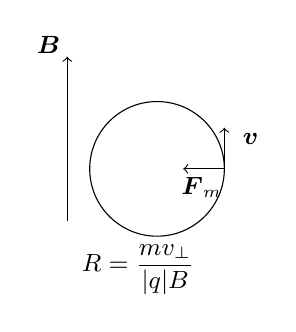
\begin{tikzpicture}[scale=0.95]
 \draw[->] (0,0) -- (0,2.2);
 \node at (-0.25,2.35) {\small \(\vb*{B}\)};
 \draw (1.2,0.7) circle (0.9);
 \draw[->] (2.1,0.7) -- (2.1,1.25);
 \node at (2.45,1.1) {\small \(\vb*{v}\)};
 \draw[->] (2.1,0.7) -- (1.55,0.7);
 \node at (1.8,0.45) {\small \(\vb*{F}_m\)};
 \node at (0.95,-0.65) {\small \(R=\dfrac{mv_\perp}{\abs{q}B}\)};
\end{tikzpicture}
\end{center}

\section{为什么磁力不做功}

磁力不做功的核心并不神秘，只来自一个几何事实：
 \(P=\vb*{F}_m\cdot \vb*{v} =q(\vb*{v}\times \vb*{B})\cdot \vb*{v}=0.\) 
因为磁力永远垂直于瞬时速度，所以它不能直接增加或减少动能，只能改变速度方向。

\bridge{这句话非常值得反复咀嚼：\textbf{磁场最擅长做的事情不是“加速”粒子，而是“把粒子的运动方向掰弯”。} 以后你看到回旋加速器、质谱仪或电子束偏转，真正起作用的，首先都是“改方向”这一件事。}

\section{洛伦兹力的几个经典应用}

\textbf{速度选择器与质谱仪。} 若带电粒子同时进入互相垂直的电场和磁场，且初速度也与两者都垂直，则当
 \(qE=qvB\) 
时，电场力与磁场力恰好平衡，粒子不发生偏转，于是可选出满足
 \(v=\frac{E}{B}\) 
的那一束粒子。这就是\textbf{速度选择器}。若再让选速后的粒子进入仅有磁场 \(B_0\) 的分析区，它们会做半径为
 \(R=\frac{mv}{|q|B_0}\) 
的圆周运动，因此
 \(\frac{m}{|q|}=\frac{BB_0R}{E}.\) 
于是不同荷质比的粒子就会走出不同半径的轨道，这正是\textbf{质谱仪}区分同位素和测量荷质比的基本思想。

\textbf{汤姆孙实验与电子荷质比。} 阴极射线管中的电子先经电压 \(V\) 加速，因此
 \(\frac12 mv^2=eV.\) 
再让电子束进入互相垂直的电场和磁场，并调到屏上\textbf{不偏转}，则有
 \(eE=evB, \qquad v=\frac{E}{B}.\) 
联立两式便得
 \(\frac{e}{m}=\frac{E^2}{2VB^2}.\) 
这条链非常值得记住，因为它告诉你：\textbf{只要能独立控制加速电压、电场和磁场，就能把不可见电子的荷质比测出来。}

\textbf{回旋加速器。} 非相对论带电粒子在匀强磁场中的回旋频率
 \(f=\frac{|q|B}{2\pi m}\) 
与速率无关。因此，只要在两个 D 形盒的缝隙间施加同频交变电场，粒子每次经过缝隙都会被\textbf{电场}再次加速，而\textbf{磁场}只负责把它弯回下一次加速位置。若 D 形盒最大半径为 \(R_0\)，则离开加速器前的最大速率与最大动能约为
 \(v_{\max}=\frac{|q|BR_0}{m}, \qquad E_{k,\max}=\frac{q^2B^2R_0^2}{2m}.\) 
这里最容易记反的一点是：\textbf{回旋加速器真正负责“增能”的是缝隙中的交变电场，不是磁场。} 磁场只改方向，不改动能。还要注意，这套“频率与速率无关”的结论只在非相对论范围内成立；当粒子速度太高时，相对论效应会让同步条件逐渐失配。

\textbf{磁聚焦（磁透镜）。} 若一束带电粒子从同一点出发，速率近似相同，但与 \(\vb*{B}\) 的夹角 \(\theta\) 都较小且略有差别，那么每个粒子都沿螺旋线前进，其节距为
 \(d=v_\parallel T =v\cos\theta\frac{2\pi m}{|q|B}.\) 
当 \(\theta\) 都不大时，\(\cos\theta\) 变化不大，各条螺旋线的节距就近似相同，于是粒子束会在后方某处再次会聚。这个现象叫\textbf{磁聚焦}，其本质就是利用洛伦兹力把电子束“整形成像”，所以它在\textbf{电子光学、电子显微镜和电子束控制}中非常重要。

\textbf{霍耳效应。} 在载流导体或半导体中，载流子带着漂移速度 \(v_d\) 前进。若外加磁场垂直于电流方向，载流子会受到横向洛伦兹力，直到横向静电场建立起来并满足
 \(|q|E_H=|q|v_dB, \qquad E_H=v_dB.\) 
若试样宽度为 \(b\)、厚度为 \(d\)，则横向霍耳电压大小为
 \(|U_H|=E_Hb=v_dBb.\) 
再由电流大小
 \(I=n|q|v_dbd\) 
可得
 \(|U_H|=\frac{IB}{n|q|d}.\) 
若把载流子电荷符号一并计入霍耳系数，则常写成
 \(U_H=R_H\frac{IB}{d}, \qquad R_H=\frac{1}{nq}.\) 
因此 \(R_H\) 的\textbf{符号}可以判断主要载流子是正电还是负电，\(R_H\) 的\textbf{大小}又能反推出载流子浓度，霍耳效应也常被用来测磁场。

\section{磁场对载流导线的作用}

导线里有大量定向运动的电荷，所以磁场对载流导线也会施力。若一小段导线元为 \(d\vb*{l}\)，电流为 \(I\)，则
 \(d\vb*{F}=I\,d\vb*{l}\times \vb*{B}.\) 
若导线为直导线且处在匀强磁场中，则总力可简化为
 \(\vb*{F}=I\vb*{L}\times \vb*{B}, \qquad F=ILB\sin\theta.\) 
之所以还能进一步写成“只看起点和终点”，关键就在于 \(\vb*{B}\) 处处相同：沿路径各小段受力虽然方向不同，但积分时真正累加出来的是整段导线的净位移，所以路径细节会被压扁成端点差。

更一般地，任意一段平面载流导线在匀强磁场中的总力只与起点和终点有关：
 \(\vb*{F} =I\int d\vb*{l}\times \vb*{B} =I(\vb*{r}_{\mathrm{end}}-\vb*{r}_{\mathrm{start}})\times \vb*{B}.\) 
于是闭合线圈满足 \(\vb*{r}_{\mathrm{end}}=\vb*{r}_{\mathrm{start}}\)，总力自然为零；这也正是为什么线圈在匀强磁场里更典型的表现不是整体平移，而是受力矩。

这里本质上仍然是洛伦兹力的集体效果：导线中每个载流子都受磁场作用，把这些微观作用沿导线加总，便得到宏观载流导线的受力结果。

\begin{remark}
两根平行载流长直导线之间还会彼此作用：同向电流相吸，反向电流相斥。这个现象本质上就是“一个电流建立磁场，再去作用另一个电流”。
\end{remark}

\section{线圈为什么会被磁场“拧转”}

单根直导线在匀强磁场里往往表现为平移受力；但闭合线圈在匀强磁场里更典型的表现是\textbf{受力矩}。这里最该先有的图像是：\textbf{电流环可以看成一个有朝向的小磁体。} 这个“小磁体想顺着外磁场转过去”的本领，一方面随电流 \(I\) 增大而增大，另一方面随围面积 \(S\) 增大而增大；而它朝向哪边，则只能靠面积法向来记录。于是先用右手定则让四指沿电流方向弯曲，拇指所指的面积法向 \(\vb*{n}\) 就定义了这只电流环的朝向。带着这个图像，再看下面两条式子才不会突兀。\bridge{这里先抓两条结论最省力：\(\vb*{m}=IS\vb*{n}\) 和 \(\vb*{M}=\vb*{m}\times\vb*{B}\)。之所以磁矩自然写成 \(IS\vb*{n}\)，是因为线圈被拧转的趋势同时随电流 \(I\) 和围面积 \(S\) 增大，而线圈正反面的区别又只能靠法向量 \(\vb*{n}\) 来记录。} 对面积为 \(S\)、电流为 \(I\)、法向单位矢量为 \(\vb*{n}\) 的线圈，定义磁矩
 \(\vb*{m}=IS\vb*{n}.\) 
它在匀强磁场中受到的力矩为
 \(\vb*{M}=\vb*{m}\times \vb*{B}, \qquad M=mB\sin\theta.\) 
若线圈有 \(N\) 匝，则
 \(M=NISB\sin\theta.\) 
这里 \(\theta\) 是线圈法向 \(\vb*{n}\) 与磁场 \(\vb*{B}\) 的夹角，所以 \(\theta=0\) 时是稳定平衡，\(\theta=\pi\) 时是不稳定平衡，\(\theta=\pi/2\) 时力矩最大。

因此线圈总会倾向于把自己的磁矩方向转到与外磁场同向的位置。这个结果和电偶极子在匀强电场中受到力矩非常相似：那边是电偶极矩 \(\vb*{p}\) 想对准 \(\vb*{E}\)，这边是磁矩 \(\vb*{m}\) 想对准 \(\vb*{B}\)。

\begin{remark}
对匀强磁场中的闭合刚性平面线圈，\textbf{合力为零、合力矩一般不为零}。这两个结论要配套记：前者告诉你线圈不必整体飞走，后者告诉你它会被“拧转”到磁矩与外磁场同向的位置。
\end{remark}

\section{磁力对电流回路做功怎样和磁通接起来}

这一节先别把它看成“又来一条新公式”，而应先认出它在回答什么问题：\textbf{当载流回路姿态或位置改变时，磁场对它做的机械功怎样用更统一的量来记？} 既然上一节已经说明线圈受力矩时会自己转去对准磁场，那么下一步最自然的追问就是：这段转动里做了多少功，能不能不用每次都从力矩积分起步？最稳的办法，是先在“匀强磁场中的线圈转动”这个最简单图景里，看力矩做功怎样一步步改写成磁通变化。

若线圈法向与磁场夹角为 \(\theta\)，则磁通量是 \(\Phi_B=BS\cos\theta\)。这时小转角 \(d\theta\) 内的元功满足
 \(dA=M\,d\theta=IBS\sin\theta\,d\theta.\) 
另一方面，
 \(d\Phi_B=d(BS\cos\theta)=-BS\sin\theta\,d\theta.\) 
这里最容易糊掉的是正负号，所以最好先固定一幅图：若线圈当前没有对准外磁场，磁力矩会把它往“磁矩更接近 \(\vb*{B}\)”的方向拧过去；在这个自发转向过程中，\(\theta\) 减小，\(\cos\theta\) 增大，因此磁通 \(\Phi_B=BS\cos\theta\) 增大。与此同时，磁场对回路做正功。也就是说，沿着“磁场自己把线圈拧过去”的实际转向看，\textbf{做正功对应的正是磁通增加。} 在这个约定下，前面两式合起来就可压成
 \(dA=I\,d\Phi_B.\) 
若把功的正负改按“外力对系统做功”来记，或者把法向与转向的约定整体反过来，式子前面的号也会一起改写。所以这里真正要先记的不是孤零零的正负号，而是\textbf{谁在做功、磁通朝哪边变}，再记最后公式。

\begin{remark}
若磁场恒定、电流也恒定，则把上式积分可得磁场对回路所做的功与磁通变化直接挂钩。这一节真正有价值的地方，不是多背一条功公式，而是建立“力矩做功也能回到磁通记账”的统一视角。
\end{remark}

\section{例题精讲}

\begin{exercise}[任意平面载流导线在匀强磁场中的总受力]
在 \(xy\) 平面内，一段任意形状的平滑导线从 \(O(0,0)\) 延伸到 \(P(L,0)\)，导线中通有电流 \(I\)。空间存在垂直纸面向里的匀强磁场 \(\vb*{B}=-B\vb*{k}\)。求整段导线所受总磁场力。
\end{exercise}

\begin{solution}
这题最值得学的不是某个特殊曲线怎么积，而是下面这个事实：\textbf{在匀强磁场中，平面载流导线的总受力只由始点、终点决定。}

设电流元
 \(d\vb*{l}=dx\,\vb*{i}+dy\,\vb*{j}.\) 
则安培力微元为
 \(d\vb*{F}=I\,d\vb*{l}\times \vb*{B} =I(dx\,\vb*{i}+dy\,\vb*{j})\times(-B\vb*{k}).\) 
逐项叉乘得
 \(d\vb*{F}=BI\,dx\,\vb*{j}-BI\,dy\,\vb*{i}.\) 
于是
 \(dF_x=-BI\,dy,\qquad dF_y=BI\,dx.\) 
沿整条导线积分：
 \(F_x=-BI\int_O^P dy=0,\) 
因为起点和终点的 \(y\) 坐标都为 \(0\)；
 \(F_y=BI\int_O^P dx=BIL,\) 
因为从 \(x=0\) 走到 \(x=L\)。

故总磁场力为
 \(\vb*{F}=BIL\,\vb*{j}.\) 
也就是说，它恰好等于那根\textbf{从 \(O\) 直连到 \(P\) 的直导线}在同一匀强磁场中所受的力。这是很多安培力积分题里最省力的捷径之一。
\end{solution}

\begin{exercise}[圆形线圈在匀强磁场中的力矩与做功]
半径为 \(R\) 的单匝圆形线圈中通有电流 \(I\)。将它放入匀强磁场中，且初始时磁场方向与线圈平面平行。求：
\begin{enumerate}
 \item 初始时线圈所受磁力矩的大小；
 \item 若线圈在磁力矩作用下转到法向与 \(\vb*{B}\) 同向，磁场力共做多少功。
\end{enumerate}
\end{exercise}

\begin{solution}
对闭合平面线圈，与其逐段算力，不如直接用磁矩
 \(\vb*{m}=IS\,\vb*{n}, \qquad S=\pi R^2.\) 
初始时磁场与线圈平面平行，故它与法向 \(\vb*{n}\) 的夹角为 \(90^\circ\)。因此总磁力矩大小为
 \(M=mB\sin 90^\circ =IB\pi R^2.\) 

再看做功。线圈转动时，若电流保持不变，磁力矩所做的功可写成
 \(A=I\Delta\Phi_B.\) 
初始时磁通量
 \(\Phi_i=BS\cos 90^\circ=0,\) 
末态时线圈法向与磁场同向，
 \(\Phi_f=BS\cos 0^\circ=BS=B\pi R^2.\) 
故
 \(A=I(\Phi_f-\Phi_i)=IB\pi R^2.\) 

这题里力矩大小和总做功恰好写成了同一个系数 \(IB\pi R^2\)，但它们的物理意义完全不同：前者是某一姿态下的“转动趋势”，后者是整个转动过程中“累计转移的能量”。
\end{solution}

\begin{exercise}[长直载流导线在匀强磁场中的受力]
一段长为 \(L\) 的直导线中通有电流 \(I\)，置于匀强磁场 \(\vb*{B}\) 中。若导线方向与磁场夹角为 \(\theta\)，求导线所受安培力。
\end{exercise}

\begin{solution}
对直导线，安培力微元
 \(d\vb*{F}=I\,d\vb*{l}\times \vb*{B}.\) 
由于整段导线方向固定、磁场又均匀，大小可以直接积出来：
 \(F=\int I B\sin\theta\,dl =IB\sin\theta\int_0^L dl.\) 
因此
 \(\boxed{F=ILB\sin\theta}.\) 
方向由 \(I\vb*{L}\times \vb*{B}\) 决定。这个式子其实就是安培力最常见的整段导线版，后面很多复杂导线题都只是把它拆回微元再积分。
\end{solution}

\begin{exercise}[有限长直导线受无限长直导线的磁场力]
一根无限长直导线中通有电流 \(I_1\)。与它共面地放置一根长为 \(L\) 的直导线，电流为 \(I_2\)。设该导线近端到长直导线的距离为 \(r\)，并与过近端的垂线夹角为 \(\alpha\)。求这根有限导线所受磁场力大小。
\end{exercise}

\begin{solution}
长直导线在距其 \(x\) 处产生的磁场大小为
 \(B(x)=\frac{\mu_0I_1}{2\pi x}.\) 
有限导线上的每一小段所受安培力方向相同，因此只需积分大小。由几何关系
 \(x=r+l\cos\alpha, \qquad dl=\frac{dx}{\cos\alpha}.\) 
于是
 \(dF=I_2B(x)\,dl =\frac{\mu_0I_1I_2}{2\pi x}\frac{dx}{\cos\alpha}.\) 
从 \(x=r\) 积到 \(x=r+L\cos\alpha\)，得
 \(F=\frac{\mu_0I_1I_2}{2\pi\cos\alpha}\int_r^{r+L\cos\alpha}\frac{dx}{x} =\frac{\mu_0I_1I_2}{2\pi\cos\alpha}\ln\frac{r+L\cos\alpha}{r}.\) 
故
 \(\boxed{ F=\frac{\mu_0I_1I_2}{2\pi\cos\alpha}\ln\frac{r+L\cos\alpha}{r} }.\) 
这题的难点纯粹是几何变量替换，本质仍是“先找外磁场，再对安培力积分”。
\end{solution}

\begin{exercise}[半圆形载流导线在匀强磁场中的受力]
半径为 \(R\) 的半圆形导线位于纸面内，电流沿圆弧从左端流向右端，空间有垂直纸面向里的匀强磁场 \(B\)。求该半圆弧所受总安培力。
\end{exercise}

\begin{solution}
逐元积分固然可做，但更快的识别是：在匀强磁场中，一段平面载流导线的总受力只由起点和终点决定。因此该半圆弧受到的总力，等于连接两端的直径导线在同一磁场中的受力。

于是直接得 \(F=IB(2R)=2IBR\)。
方向由电流方向与磁场方向的叉乘决定；按题设取向，它与直径垂直并指向半圆开口一侧。这个结果很好地说明了“匀强磁场里算整段导线受力，别总想着沿曲线死积分”。
\end{solution}

\begin{exercise}[圆形线圈在指定坐标系中的磁力矩方向]
一半径为 \(R\) 的可转动圆形线圈中通有电流 \(I\)，线圈法向沿 \(+z\) 方向，匀强磁场 \(\vb*{B}=B\vb*{i}\)。求线圈所受磁力矩。
\end{exercise}

\begin{solution}
线圈磁矩为
 \(\vb*{m}=IS\,\vb*{k}=I\pi R^2\,\vb*{k}.\) 
所以
 \(\vb*{M}=\vb*{m}\times \vb*{B} =I\pi R^2\,\vb*{k}\times B\vb*{i} =I\pi R^2B\,\vb*{j}.\) 
故
 \(\boxed{\vb*{M}=I\pi R^2B\,\vb*{j}}.\) 
这题提醒我们：很多线圈受力矩题里，大小并不难；先把磁矩方向判对，再用叉乘一把得到方向，方向关系才不会乱。
\end{solution}

\begin{exercise}[圆电流与共面长直导线间的安培力]
一根无限长直导线与半径为 \(R\)、电流为 \(I\) 的圆电流共面放置，并沿圆的一条直径方向通过。长直导线电流为 \(I_0\)。求：
\begin{enumerate}
 \item 圆上半弧所受总安培力；
 \item 整个圆电流所受总安培力。
\end{enumerate}
\end{exercise}

\begin{solution}
对位于半圆弧上的电流元，长直导线在其处产生的磁场大小为
 \(B=\frac{\mu_0 I_0}{2\pi x},\) 
其中 \(x=R\sin\theta\)。安培力微元为 \(d\vb*{F}=I\,d\vb*{l}\times\vb*{B}\)，把它沿直径方向取分量后，垂直于直径的分量由对称性相互抵消，而留下的分量满足
\[
\begin{aligned}
dF_{\parallel}
&=IB\,dl\,\sin\theta
=I\frac{\mu_0I_0}{2\pi R\sin\theta}R\,d\theta\,\sin\theta
=\frac{\mu_0I_0I}{2\pi}\,d\theta,\\
F_{\text{半弧}}
&=\int_0^\pi dF_{\parallel}
=\frac{\mu_0 I_0 I}{2}.
\end{aligned}
\]
而对整个圆电流，同样的积分在上下两半圆上同向叠加，因此
\[
F_{\text{全圆}}=\mu_0 I_0 I.
\]
故
\[
\boxed{
F_{\text{半弧}}=\frac{\mu_0 I_0 I}{2},
\qquad
F_{\text{全圆}}=\mu_0 I_0 I.
}
\]
这类题看起来像“奇怪几何”，本质还是两步：先写出长直导线的磁场，再利用对称性删去会互相抵消的分量。
\end{solution}

\section{本章方法提要}

涉及磁场力时，最稳的顺序是：
\begin{enumerate}
 \item 先看研究对象：单个电荷、整段导线，还是闭合线圈；
 \item 再看 \(\vb*{v}\) 或 \(d\vb*{l}\) 与 \(\vb*{B}\) 的夹角；
 \item 然后先画方向图，再代数计算大小；
 \item 一旦题目问能量或速率变化，立刻回想“磁力不做功”，看它到底能改什么、不能改什么。
\end{enumerate}

\section{常见误区}

\begin{itemize}
 \item 把磁力方向错画成沿 \(\vb*{v}\) 或沿 \(\vb*{B}\)。
 \item 误以为“只要有磁力就一定会越来越快”。磁力改方向，不直接改动能。
 \item 把载流导线受力和平行导线相互作用混成两套无关公式，忘了它们都来自 \(I\,d\vb*{l}\times \vb*{B}\)。
 \item 看到线圈就只算总力，忽略真正支配转动的是力矩。
\end{itemize}

\section{章末小结}

\summaryline{磁场对运动电荷的作用由洛伦兹力给出，它总垂直于速度，所以最擅长“拐弯”而不是“增速”；速度选择器、质谱仪、汤姆孙实验、回旋加速器和霍耳效应都只是这同一条力学主线在不同装置中的展开；对载流导线，微观洛伦兹力加总成宏观磁场力；对闭合线圈，又进一步表现为磁矩在外磁场中的受力矩。}
\chapterselfcheck{为什么匀强磁场能让粒子做圆周或螺旋运动，却不直接改动能？为什么回旋加速器里真正负责增加动能的是电场而不是磁场？为什么霍耳电压的符号能判断载流子类型？遇到电子在磁场中偏转的题，为什么一定要先画方向图？}

\chapter{磁介质}

\begin{skill}[第18章冲刺总手册]\label{sk:phys-ch18-overview}
 这章处理“材料放进磁场后，外磁场和介质自身响应怎样分账”的题。核心不是再造一套新力学，而是把 \(\vb*{B},\vb*{H},\vb*{M}\) 各自管什么说清。
 题面若出现“磁化强度、磁介质、顺磁、抗磁、铁磁、自由电流、束缚电流、磁化电流、磁场强度”，就说明题目要你区分“外部电流造成的场”和“介质被磁化后的附加响应”。

\[
\begin{aligned}
\oint_L \vb*{H}\cdot \dd \vb*{l}&=I_{\mathrm{free}},\\
\vb*{B}&=\mu_0(\vb*{H}+\vb*{M}).
\end{aligned}
\]
先用 \(\vb*{H}\) 盯住自由电流，再用 \(\vb*{M}\) 把介质响应补回到 \(\vb*{B}\)。

\[
\begin{aligned}
\vb*{B}&=\mu_0(\vb*{H}+\vb*{M}),\\
\vb*{M}&=\chi_{\mathrm m}\vb*{H}
\quad \text{(线性各向同性磁介质)},\\
\vb*{B}&=\mu \vb*{H}
=\mu_0(1+\chi_{\mathrm m})\vb*{H}
=\mu_r\mu_0\vb*{H},\\
\oint_L \vb*{H}\cdot \dd \vb*{l}&=I_{\mathrm{free}},\qquad
\oint_S \vb*{B}\cdot \dd \vb*{S}=0.
\end{aligned}
\]
这里 \(\chi_{\mathrm m}\) 是磁化率，\(\mu_r\) 是相对磁导率；\(\vb*{H}\) 主要追踪自由电流，\(\vb*{B}\) 才是最后真正参与受力和磁通量的场。
 先看题目给的是自由电流、总磁感应强度还是材料参数；若几何对称明显，先用 \(\oint \vb*{H}\cdot\dd\vb*{l}=I_{\mathrm{free}}\) 求 \(\vb*{H}\)；再由材料关系求 \(\vb*{M}\) 或 \(\vb*{B}\)。若题目只在讨论磁介质前后同一装置中场的变化，就重点比较 \(\mu_r\) 进入后哪些量按比例变化。
 把 \(\vb*{H}\) 和 \(\vb*{B}\) 当成完全等价；见到介质后仍直接把安培环路定理写成 \(\oint \vb*{B}\cdot \dd\vb*{l}=\mu_0 I_{\mathrm{free}}\) 而不交代条件；把顺磁、抗磁的差别记反；忘记磁介质里仍满足 \(\nabla\cdot \vb*{B}=0\)。
 看结果是否符合材料直觉：顺磁或铁磁应增强同向磁感应，抗磁应减弱；看无介质极限 \(\mu_r\to 1\) 时是否回到真空结果；量纲上 \(\vb*{B}\) 是 \(\mathrm T\)，\(\vb*{H}\) 是 \(\mathrm{A/m}\)，不要混写。
\end{skill}

\chapterroadmap
{回答“物质进入磁场后怎样被磁化”，并把 \(\vb*{B},\vb*{H},\vb*{M}\) 三个量的分工理顺。}
{已经知道电流建立磁场、磁场作用于运动电荷和电流。}
{新增磁化、磁化电流、磁场强度 \(\vb*{H}\)、介质中的安培环路定理，以及抗磁/顺磁/铁磁的差异。}

\bridge{静电学里，电介质进入外场会极化；磁学里，磁介质进入外场会磁化。于是 \(\vb*{B}\) 不再只由自由电流决定，还会受到介质内部微观磁矩取向变化的影响。学这一章的关键，就是把“自由电流造的那部分场”和“介质自己响应出来的那部分场”分开记账。}

\section{磁化与磁矩}

前面一直在宏观上讨论“外部电流怎样造场”；下面为了说明材料为什么会自己补出一份磁场，必须暂时切到微观磁矩图像。

从微观上看，很多原子、分子或电子轨道本身就可等效为小电流环。只要有电流环，就会自然带有磁矩：
 \(\vb*{m}=IS\,\vb*{n},\) 
其中 \(I\) 是等效环流，\(S\) 是环面积，方向 \(\vb*{n}\) 由右手定则给出。也就是说，磁矩并不是凭空冒出来的抽象矢量，而是在把“这一小圈电流想把自己朝哪边摆”浓缩成一个方向和大小。没有外磁场时，这些微观磁矩往往取向杂乱，宏观平均后磁效应不明显；加上外磁场后，部分磁矩趋于定向排列，宏观上就表现为磁化。

磁化强度记作 \(\vb*{M}\)，它描述单位体积内净磁矩的平均分布，可写成
 \(\vb*{M}=\frac{d\vb*{m}}{dV}.\) 
虽然教材上它看起来只是“又一个新矢量”，但物理意义非常明确：\textbf{它刻画的是介质内部自己贡献出来的磁性部分。} 若把介质想成许多微观小电流环排队，\(\vb*{M}\) 就是在记“这些小电流环到底排得有多整齐、总体更偏向哪边”。

\bridge{若把磁化想成大量微观小电流环重新排队，就会发现一个很关键的几何事实：相邻小电流环在内部边界上的电流会彼此抵消，真正留下来的主要是外表面的等效环流。因此磁化不仅可以用“磁矩取向”来讲，也可以用“等效磁化电流”来讲。}

\begin{note}
\textbf{记方向时最稳的办法是先想右手定则：} 四指沿等效环流方向弯过去，大拇指所指就是磁矩方向，也是宏观磁化强度 \(\vb*{M}\) 的方向。这样就不会把“磁矩指向”和“电流绕行方向”混成两套互不相干的规定。
\end{note}

真正做题时，并不是要把所有微观电流逐个算出来，而是把一束平行排开的微观电流环粗略打包：回路真正统计到的是净剩下的边界环流，所以才会出现“\(\vb*{M}\) 的环量 = 围住的等效电流”这类关系。

若取一条闭合回路 \(L\) 围住介质的一部分，则磁化强度与等效磁化电流满足
 \(\oint_L \vb*{M}\cdot d\vb*{l}=\sum I_s,\) 
这里 \(\sum I_s\) 表示被回路围住的等效磁化电流代数和。这个关系的价值在于：它把抽象的 \(\vb*{M}\) 重新翻译回了我们已经熟悉的“电流造磁场”语言。

\section{磁场强度 H 与介质中的安培环路定理}

这里第一次最容易卡的是：明明已经有了 \(\vb*{B}\) 和 \(\vb*{M}\)，为什么又要再来一个 \(\vb*{H}\)？最稳的想法是先把目标说死：\textbf{若题目要你按自由电流来写环路定理，就必须有一个量能把磁化那一部分先剥出去。} 这时三者分工就清楚了：\(\vb*{M}\) 记的是材料自身磁化，也就是“单位体积净磁矩”；\(\vb*{B}\) 记的是最后真正参与受力、决定磁通的总磁场；\(\vb*{H}\) 则像静电学里的 \(\vb*{D}\) 一样，是为了把\textbf{自由电流源单独拎出来记账}而引入的辅助场。为了把“自由电流贡献”和“磁化贡献”分账，引入磁场强度 \(\vb*{H}\)。在真空中，
 \(\vb*{B}=\mu_0\vb*{H};\) 
在一般介质中，
 \(\vb*{B}=\mu_0(\vb*{H}+\vb*{M}).\) 
它不是凭空多造一个字母，而是从“总环量怎样拆账”这件事里被逼出来的。因为介质中
 \(\oint_L \vb*{B}\cdot d\vb*{l} =\mu_0\left(\sum I_{\mathrm{free}}+\sum I_s\right) =\mu_0\left(\sum I_{\mathrm{free}}+\oint_L \vb*{M}\cdot d\vb*{l}\right).\) 
既然右边第二项正是“介质自己响应出来的那本账”，那就把它移到左边，让左边只剩自由电流对应的部分，于是
 \(\vb*{H}=\frac{\vb*{B}}{\mu_0}-\vb*{M}, \qquad \oint_L \vb*{H}\cdot d\vb*{l}=I_{\mathrm{free}}.\) 
对各向同性线性均匀磁介质，还可以进一步写成
 \(\vb*{M}=\chi_m \vb*{H}, \qquad \vb*{B}=\mu\vb*{H},\) 
其中 \(\mu=\mu_0(1+\chi_m)\) 为磁导率。

于是安培环路定理在介质中最实用的写法变成
 \(\oint_L \vb*{H}\cdot d\vb*{l}=I_{\mathrm{free}}.\) 

\begin{note}
\textbf{这和电介质里引入 \(\vb*{D}\) 的思路完全平行：} \(\vb*{B}\) 对总磁效应负责，\(\vb*{H}\) 主要对自由电流负责。以后只要介质一出现，就不要再把真空中的单一本构关系机械照搬。
\end{note}

\section{三类常见磁介质：抗磁、顺磁、铁磁}

\bridge{这一节最怕被读成名词表。更自然的是看材料内部的小磁矩在外场来之前和来了之后分别会怎样：有的材料本来几乎没有可稳定排队的永久磁矩，只会被外场轻微诱导反向响应；有的本来就有微观磁矩，但只能弱弱地顺着外场多排一点；还有的内部早就分成一块块磁畴，外场一来会成片翻转，甚至留下明显历史记忆。也正因为微观机制不同，宏观上才会分成抗磁、顺磁和铁磁三类。}

\begin{itemize}
 \item \textbf{抗磁质：} 外场使感生磁矩方向与外场相反，磁化很弱，\(\mu_r\) 略小于 1。
 \item \textbf{顺磁质：} 原有磁矩在外场中略趋同向，磁化较弱，\(\mu_r\) 略大于 1。
 \item \textbf{铁磁质：} 内部存在磁畴结构，外场可使磁畴大范围重排，因此磁化很强，\(\mu_r\) 可远大于 1。
\end{itemize}

铁磁质之所以特殊，不只是“磁化更大”，而是它具有明显的历史效应：外场撤去后，磁化不一定立刻完全消失，于是出现剩磁、矫顽力和磁滞回线等现象。

\section{磁滞与软磁、硬磁材料}

铁磁材料里，\(\vb*{B}\) 与 \(\vb*{H}\) 之间常不再是一条简单直线，而是随加磁、退磁历史出现磁滞回线。回线窄、矫顽力小的材料适合做铁芯等反复磁化退磁的器件，常称\textbf{软磁材料}；回线宽、剩磁大的材料适合做永久磁体，常称\textbf{硬磁材料}。

\begin{remark}
这里最容易被忽略的是：铁磁质不是“\(\mu\) 特别大”的单纯线性介质，而是一类具有磁畴结构、非线性和历史记忆效应的材料。
\end{remark}

\section{例题精讲}

\begin{exercise}[\(H\) 与 \(B\) 的分段分工]
一半径为 \(R_1\) 的无限长圆柱导线外包一层外半径为 \(R_2\)、相对磁导率为 \(\mu_r\) 的均匀磁介质圆筒。导线中通有电流 \(I\)，且电流在导线截面上均匀分布。求各区域中的磁场强度 \(H(r)\) 与磁感应强度 \(B(r)\)。
\end{exercise}

\begin{solution}
这题最关键的观念不是一上来就算 \(B\)，而是先记住：\textbf{\(\vb*{H}\) 主要由自由电流决定，\(\vb*{B}\) 再由介质响应放大或缩小。}

先用半径为 \(r\) 的圆形安培回路。由对称性，\(\vb*{H}\) 沿回路切向且大小恒定，于是
 \(\oint \vb*{H}\cdot d\vb*{l}=H(2\pi r)=I_{\mathrm{free,enc}}.\) 

当 \(0<r<R_1\) 时，包围的自由电流仅占总电流的面积比：
 \(I_{\mathrm{enc}}=I\frac{r^2}{R_1^2}.\) 
故
 \(H(r)=\frac{Ir}{2\pi R_1^2}, \qquad B(r)=\mu_0H(r)=\frac{\mu_0Ir}{2\pi R_1^2}.\) 
这里仍在导线本体内部，尚未进入外包磁介质，所以 \(B=\mu_0H\)。

当 \(R_1<r<R_2\) 时，回路已包围全部自由电流 \(I\)，因此
 \(H(r)=\frac{I}{2\pi r}.\) 
但这一区域位于磁介质中，所以
 \(B(r)=\mu H(r)=\mu_0\mu_r\frac{I}{2\pi r}.\) 

当 \(r>R_2\) 时，回路外侧回到真空（或空气），包围自由电流仍是 \(I\)，所以
 \(H(r)=\frac{I}{2\pi r}, \qquad B(r)=\mu_0\frac{I}{2\pi r}.\) 

综上，
\[
H(r)=
\begin{cases}
\dfrac{Ir}{2\pi R_1^2}, & 0<r<R_1,\\[6pt]
\dfrac{I}{2\pi r}, & r>R_1,
\end{cases}
\]
\[
B(r)=
\begin{cases}
\dfrac{\mu_0Ir}{2\pi R_1^2}, & 0<r<R_1,\\[6pt]
\dfrac{\mu_0\mu_rI}{2\pi r}, & R_1<r<R_2,\\[6pt]
\dfrac{\mu_0I}{2\pi r}, & r>R_2.
\end{cases}
\]

这正体现了 \(\vb*{H}\) 与 \(\vb*{B}\) 的分工：\(\vb*{H}\) 先把自由电流的“源账”做好，\(\vb*{B}\) 再通过不同区域的本构关系体现介质影响。
\end{solution}

\begin{exercise}[充满磁介质的长直螺线管]
一长直密绕螺线管内充满相对磁导率为 \(\mu_r\) 的均匀磁介质，单位长度匝数为 \(n\)，通有电流 \(I\)。求管内磁感应强度。
\end{exercise}

\begin{solution}
先对 \(\vb*{H}\) 用安培环路定理。取一条跨越螺线管内外的矩形回路，由于长螺线管外部磁场近似很小，内部 \(\vb*{H}\) 近似均匀，故
 \(Hl=nIl \quad\Longrightarrow\quad H=nI.\) 
再由线性磁介质中的本构关系
 \(B=\mu H=\mu_0\mu_r H\) 
得到
 \(\boxed{ B=\mu_0\mu_r nI }.\) 
这题最能说明“先算 \(H\)，再转成 \(B\)”的好处：自由电流决定 \(H\)，介质参数只在最后一步进入。
\end{solution}

\begin{exercise}[两同轴反向电流圆筒间的磁场]
有两个半径分别为 \(R_1,R_2\) 的无限长同轴圆筒形导体，之间充满相对磁导率为 \(\mu_r\) 的均匀磁介质。两圆筒中通有大小相等、方向相反的电流 \(I\)。求各区域磁感应强度。
\end{exercise}

\begin{solution}
对三段区域分别用安培环路定理求 \(\vb*{H}\)：

当 \(r<R_1\) 时，回路不包围净自由电流，故
 \(H=0,\qquad B=0.\) 

当 \(R_1<r<R_2\) 时，回路只包围内圆筒电流 \(I\)，故
 \(H\cdot 2\pi r=I \quad\Longrightarrow\quad H=\frac{I}{2\pi r}.\) 
此区在磁介质内，所以
 \(B=\mu_0\mu_r H =\frac{\mu_0\mu_r I}{2\pi r}.\) 

当 \(r>R_2\) 时，回路同时包围 \(+I\) 和 \(-I\)，净自由电流为零，因此
 \(H=0,\qquad B=0.\) 
故
\[
\boxed{
B(r)=
\begin{cases}
0, & r<R_1,\\[4pt]
\dfrac{\mu_0\mu_r I}{2\pi r}, & R_1<r<R_2,\\[6pt]
0, & r>R_2.
\end{cases}}
\]
它和同轴电缆的电场分布非常像，只不过这里是磁场，而且由反向电流把场锁在两圆筒之间。
\end{solution}

\section{本章方法提要}

磁介质题通常这样展开：
\begin{enumerate}
 \item 先问题目是在\textbf{算场}，还是在\textbf{认材料行为}；
 \item 若是算场，先把自由电流与介质响应分账：优先用
 \(\oint \vb*{H}\cdot d\vb*{l}=I_{\mathrm{free}}\) 
 去锁自由电流贡献，再回到 \(\vb*{M}\) 与 \(\vb*{B}\)；
 \item 若介质可近似看作线性、各向同性、均匀介质，就顺着
 \(\vb*{M}=\chi_m\vb*{H}, \qquad \vb*{B}=\mu\vb*{H}\) 
 这条链往下走；
 \item 若题目谈的是铁磁质、磁滞、剩磁、矫顽力，就不要再把它当成“\(\mu\) 很大的线性材料”，而应切到磁畴与历史效应的语言。
\end{enumerate}

\begin{note}
\textbf{这一章最值得死记的不是某个单独公式，而是三者分工：} \(\vb*{B}\) 描写总磁效应，\(\vb*{H}\) 主要对自由电流记账，\(\vb*{M}\) 描写介质自己的磁化响应。很多介质题一旦把这三者混成一个量，后面几乎必乱。
\end{note}

\section{常见误区}

\begin{itemize}
 \item 把 \(\vb*{B}\) 和 \(\vb*{H}\) 当成同一个量，只差一个单位。
 \item 在介质题里仍然机械使用真空关系 \(B=\mu_0H\)。
 \item 以为顺磁、抗磁、铁磁的区别只是“强弱不同”，忽略铁磁质的磁畴和磁滞特性。
 \item 以为磁化意味着材料内部真的有宏观电荷流在绕圈跑；更准确地说，它是微观磁矩平均取向变化的宏观表述。
\end{itemize}

\section{章末小结}

\summaryline{磁介质进入外磁场后会磁化，于是磁场分成“自由电流建立的部分”和“介质响应建立的部分”两本账。用 \(\vb*{H}\) 可以更方便地追踪前者，用 \(\vb*{M}\) 则描述后者；而铁磁质之所以特殊，关键在于磁畴重排和磁滞。}
\chapterselfcheck{为什么介质题里要把 \(\vb*{B}\)、\(\vb*{H}\)、\(\vb*{M}\) 分开？为什么铁磁质不能简单看成“\(\mu\) 很大的线性介质”？为什么介质中的安培环路定理更适合写成关于 \(\vb*{H}\) 的形式？}

\chapter{电磁感应}

\begin{skill}[第19章冲刺总手册]\label{sk:phys-ch19-overview}
 这章解决“为什么回路里会自己冒出电动势”的题。所有题都绕不开一个判断：磁通量为什么变了，是磁场变、面积变、姿态变，还是导体在切割磁感线。
 题面若出现“线圈穿过磁场”“磁通量变化”“感应电流方向”“导杆滑动”“自感、互感”“回路中电流随时间变化”，先把“谁导致磁通变化”圈出来。

\[
\begin{aligned}
\Phi_B&=\int_S \vb*{B}\cdot \dd \vb*{S},\\
\mathcal{E}&=-\dv{\Phi_B}{t}.
\end{aligned}
\]
先找磁通量，再谈符号；楞次定律本质上就是这个负号的物理解释。

\[
\begin{aligned}
\Phi_B&=\int_S \vb*{B}\cdot \dd \vb*{S}
\ \Rightarrow\ 
\Phi_B=BS\cos\theta\ \text{(匀强磁场平面回路)},\\
\mathcal{E}&=-\dv{\Phi_B}{t},\qquad
\mathcal{E}_{\text{动生}}=Blv\ \text{(导杆垂直切割时)},\\
\mathcal{E}_L&=-L\dv{I}{t},\qquad
\mathcal{E}_{21}=-M\dv{I_1}{t},\\
W_m&=\frac12 LI^2.
\end{aligned}
\]
其中 \(L\) 是自感系数，\(M\) 是互感系数；动生电动势公式 \(Blv\) 只是法拉第定律在特定几何下的短写。
 先明确回路和取正方向，再写 \(\Phi_B\)；接着判断通量变化来自 \(B,S,\theta\) 哪一个，必要时把 \(\Phi_B=BS\cos\theta\) 分别对时间求导；然后用楞次定律判感应电流方向，最后再联立欧姆定律或回路方程求电流、功率、外力。遇到自感题，直接把 \(-L\dfrac{\dd I}{\dd t}\) 写进回路方程。
 一上来背楞次定律口号，却没先说明磁通到底怎样变化；把磁通量变化误当成只看 \(B\) 变化；动生电动势里速度方向、导杆方向、磁场方向三者不互相垂直时仍机械套 \(Blv\)；把自感电动势方向写成“总是与电流反向”，其实它反抗的是电流变化。
 看感应效应是否真的阻碍原变化：磁通增大时感应磁场应设法减小它，磁通减小时感应磁场应设法补回来；量纲上电动势是伏特；若导杆做匀速切割，外力做功应与回路发热或电磁能增加对应上。
\end{skill}

\chapterroadmap
{把“变化的磁场”与“感应电动势”接起来，理解法拉第定律、楞次定律、动生/感生电动势，以及自感、互感和磁场能量。}
{已经会描述稳恒电流和静磁场，也知道磁场对电荷和电流的作用。}
{新增磁通量、法拉第电磁感应定律、非静电力场、自感/互感与磁场能量。}

\bridge{前面磁学讨论的大多是“电流产生磁场、磁场作用电流”；这一章出现真正的双向耦合：变化的磁场反过来又能生电场和电流。法拉第定律因此是电磁学从“静态章节并列”走向“动态统一理论”的关键转折。}

\section{磁通量与法拉第电磁感应定律}

这一节真正该先想清楚的是：回路里出现感应电流，不是因为“磁场神秘地产生了电”，而是因为\textbf{穿过回路的总磁场联系正在变化}。若回路所围面积、姿态、或空间磁场本身随时间变了，那么“回路和磁场的联系量”就不再固定，于是系统会用感应电动势来反抗这种变化。这个“联系量”就是磁通。

穿过某曲面的磁通量定义为
 \(\Phi_B=\int_S \vb*{B}\cdot d\vb*{S}.\) 
若回路所围曲面的磁通量随时间变化，则回路中会出现感应电动势：
 \(\mathcal{E}=-\dv{\Phi_B}{t}.\) 
这就是\textbf{法拉第电磁感应定律}。

这里的负号不是装饰，而是\textbf{楞次定律}的数学体现：感应电流总要反抗原磁通变化。若原磁通在增大，感应电流建立的磁场就倾向于让它减小；若原磁通在减小，感应电流就倾向于把它“补回来”。

\begin{remark}
真正判断方向时，最稳的做法是：\textbf{先任选回路绕行方向，再按右手螺旋给穿过回路的磁通规定正方向。} 若算得 \(\mathcal{E}>0\)，说明感应电动势方向与所选绕向一致；若算得 \(\mathcal{E}<0\)，则实际方向与所选绕向相反。这样负号就不再神秘，而是清楚地落实到方向约定上。
\end{remark}

若线圈有 \(N\) 匝，更自然的记账量是\textbf{磁通链}
 \(\Psi=N\Phi_B, \qquad \mathcal{E}=-\dv{\Psi}{t}.\) 

\section{动生电动势与感生电动势}

在写公式前，最好先把两种来源分开：若是导体自己在磁场里切割磁感线，真正推动电荷的是载流子随导体运动时受到的洛伦兹力，这叫动生；若导体不动但磁场自己在变，则空间里会出现环形感应电场去推电荷，这叫感生。两种机制的表面现象都叫“有感应电动势”，但第一推手并不是同一个。

磁通变化有两种典型来源：
\begin{itemize}
 \item 回路本身在磁场中运动或形变，这时常称\textbf{动生电动势}；
 \item 回路不动，但空间磁场随时间变化，这时常称\textbf{感生电动势}。
\end{itemize}

对长度为 \(l\) 的金属棒以速度 \(v\) 垂直切割匀强磁场时，有经典结果
 \(\mathcal{E}=Blv.\) 
更一般地，动生电动势可写成
 \(\mathcal{E}=\int (\vb*{v}\times \vb*{B})\cdot d\vb*{l}.\) 
而感生电动势的本质，则是变化磁场激发了非静电感应电场，使得沿闭合回路
 \(\oint \vb*{E}_{\mathrm{ind}}\cdot d\vb*{l}=-\dv{\Phi_B}{t}.\) 

\begin{exercise}
设半径为 \(R\) 的长螺线管内部磁场 \(B(t)\) 近似均匀，管外磁场近似忽略。若取与轴同心、半径为 \(r\) 的圆形回路，则感生电场沿环向分布，并满足
 \(2\pi r E_\varphi=-\pi r^2\dv{B}{t}, \qquad r<R,\) 
故
 \(E_\varphi(r)=-\frac{r}{2}\dv{B}{t}.\) 
若 \(r>R\)，穿过回路的磁通只由半径 \(R\) 的内部磁场决定，于是
 \(2\pi r E_\varphi=-\pi R^2\dv{B}{t}, \qquad E_\varphi(r)=-\frac{R^2}{2r}\dv{B}{t}.\) 
这说明感生电场并不只存在于“有磁场的地方”，而是以闭合场线的形式分布在更广的空间区域中。换句话说，它的电场线不是从正电荷出发、到负电荷终止，而是绕着变化磁通围成一圈圈与螺线管同轴的闭合同心圆。
\end{exercise}

\begin{remark}
动生电动势的“非静电力来源”可以直接追到洛伦兹力；感生电动势则更深一步，说明即使没有导体整体运动，变化磁场本身也能在空间中建立有旋电场。
\end{remark}

\begin{remark}
也正因为感生电场本身就真实存在，所以即使导体整体静止、甚至不是完整闭合回路，导体两端也可能测得感应电动势；若把大块导体放入时变磁场中，内部还会自动围成许多闭合感应电流回路，这就是\textbf{涡电流}。它一方面会带来额外焦耳热，另一方面又能产生电磁阻尼，所以工程上常通过叠片、开槽等方式削弱涡流回路面积。
\end{remark}

\section{自感与互感}

这一节读公式前最重要的一句判断是：电流变化最先改写的是磁通，而磁通变化又会反过来阻碍这种电流变化本身。所以无论自感还是互感，本质上都不是“突然多了一个常数 \(L\) 或 \(M\)”，而是“电流 \(\rightarrow\) 磁通 \(\rightarrow\) 反向感应电动势”这条回路被压成了比例关系。

如果同一回路中的电流变化引起本回路磁通变化，就会在自身回路中产生感应电动势，这叫\textbf{自感}。更严谨地说，应先定义磁通链 \(\Psi\)，再写
 \(\Psi=LI, \qquad \mathcal{E}_L=-L\dv{I}{t}.\) 
若线圈有 \(N\) 匝，则 \(\Psi=N\Phi_B\)。只有在单匝或已默认按磁通链记账时，才可把它简写成“\(\Phi\) 与 \(I\) 成正比”的样子。

若一个回路中的电流变化，引起另一个回路中磁通变化并产生感应电动势，则叫\textbf{互感}。同样应先写成
 \(\Psi_{21}=MI_1, \qquad \mathcal{E}_{21}=-M\dv{I_1}{t}.\) 

\begin{note}
自感和互感的核心物理意义都是“电流变化引起磁通变化，再由磁通变化反过来阻碍这种变化”。这也是为什么很多电感元件表现出“电流不愿突然变化”的惯性。
\end{note}

\section{磁场能量}

这里先别把 \(W_m=\frac12 LI^2\) 当成又一条孤立结果。真正该先想的是：建立电流时，外界明明在持续对抗自感电动势做功，而一旦电流稳定后，这部分功并没有凭空消失，只能被储存在某个地方。电磁学前面已经反复提醒过我们，能量不只贴在粒子或元件上，也可以分布在空间中的场里。所以磁场能量公式本质上是在回答：\textbf{刚才那部分克服自感做下去的功，最后记到了磁场账上。}

建立电流要克服自感电动势，因此外界做功会储存在磁场中。对电感元件，
 \(W_m=\frac{1}{2}LI^2.\) 
若进一步写成场的形式，在真空中常用
 \(w_m=\frac{B^2}{2\mu_0},\) 
在一般线性介质中则更自然地写成
 \(w_m=\frac{1}{2}\vb*{B}\cdot \vb*{H}.\) 

\bridge{电场里有 \(\frac12 \vb*{E}\cdot \vb*{D}\)，磁场里有 \(\frac12 \vb*{B}\cdot \vb*{H}\)。这再次提醒我们：电磁学越来越倾向于把能量理解成\textbf{场分布}，而不是只贴在元件或粒子本身。}

\section{例题精讲}

\begin{exercise}[滑动导杆的感应电动势]
矩形闭合导体回路的一边 \(ab\) 长为 \(l\)，可在导轨上无摩擦滑动。整个回路处在垂直于回路平面、大小为 \(B\) 的匀强磁场中。若导杆 \(ab\) 以恒定速度 \(v\) 向右滑动，求回路中的感应电动势。
\end{exercise}

\begin{solution}
这类题不要先背 \(Blv\)，而应由题意追问“\textbf{磁通为什么在变}”。这里 \(B\) 不变，夹角不变，真正变化的是回路面积。

设时刻 \(t\) 时导杆位置对应回路宽度为 \(x\)，取顺时针绕行为正，则 \(\Phi_B=BS=Blx\)，于是 \(\mathcal{E}=-\dv{\Phi_B}{t}=-Bl\dv{x}{t}=-Blv\)，所以感应电动势大小为 \(\abs{\mathcal{E}}=Blv\)。
负号表示：若我们把顺时针取作正方向，那么真实感应电流方向与之相反，即为\textbf{逆时针方向}。这和楞次定律完全一致，因为导杆右移使回路面积增大，原磁通增强，于是感应电流必须建立一个反抗这种增强的磁场。
\end{solution}

\begin{exercise}[时变长直电流在线圈中激发的感应电动势]
一根无限长直导线中通有电流
 \(i(t)=I_0\sin\omega t.\) 
导线旁有一个与之共面的矩形线圈，线圈靠近导线的一边距导线为 \(r\)，沿径向宽度为 \(l_1\)，沿导线方向长度为 \(l_2\)。求线圈中的感应电动势。
\end{exercise}

\begin{solution}
长直导线在距其 \(x\) 处产生的磁场大小为
 \(B(x,t)=\frac{\mu_0 i(t)}{2\pi x} =\frac{\mu_0 I_0\sin\omega t}{2\pi x}.\) 
矩形线圈中每条与导线平行的窄条面积元可写成 \(dS=l_2\,dx\)，故穿过线圈的总磁通为
 \(\Phi_B =\int_r^{r+l_1} B(x,t)\,l_2\,dx =\frac{\mu_0 I_0l_2}{2\pi}\sin\omega t \int_r^{r+l_1}\frac{dx}{x}.\) 
于是
 \(\Phi_B =\frac{\mu_0 I_0l_2}{2\pi}\ln\frac{r+l_1}{r}\,\sin\omega t.\) 
对时间求导即得感应电动势：
 \(\mathcal{E} =-\dv{\Phi_B}{t} =-\frac{\mu_0 I_0l_2\omega}{2\pi}\ln\frac{r+l_1}{r}\,\cos\omega t.\) 

这个结果特别适合拿来训练“磁通变化来源”的辨认：这里面积不变、姿态不变、线圈不动，\textbf{唯一在变的是源电流，从而磁场随时间变。} 一旦识别出这点，后面就是“先求磁通，再对时间求导”的固定套路。
\end{solution}

\begin{exercise}[2010级大物II：变流圆环中心小线圈的感应电动势]
半径为 \(r\) 的小绝缘圆环置于半径为 \(R\) 的大导线圆环中心，二者在同一平面内，且 \(r\ll R\)。大导线环中通有电流 \(I=t\)（单位为安培），其中 \(t\) 为时间。求任一时刻小线环中感应电动势的大小。
\end{exercise}

\begin{solution}
小环半径远小于大环半径，所以可把大环在圆心附近产生的磁场近似看成均匀场。源电流随时间线性变化，磁通随之变化。

大圆环在中心处的磁场大小为
 \(B=\frac{\mu_0 I}{2R}.\) 
由于 \(r\ll R\)，穿过小圆环的磁通近似为
 \(\Phi_B=B\cdot \pi r^2 =\frac{\mu_0 I}{2R}\pi r^2.\) 
感应电动势大小为
 \(\abs{\mathcal{E}} =\left|\dv{\Phi_B}{t}\right| =\frac{\mu_0\pi r^2}{2R}\left|\dv{I}{t}\right|.\) 
题中 \(I=t\)，故 \(\dv*{I}{t}=1\)，于是
 \(\boxed{ \abs{\mathcal{E}}=\frac{\mu_0\pi r^2}{2R} }.\) 
这里的近似条件 \(r\ll R\) 很关键；若小环不够小，就不能把大环磁场在整个小环面积上看作常量。
\end{solution}

\begin{exercise}[运动矩形线框在长直电流磁场中的感应电动势]
一矩形导体线框与一根无限长直导线共面。线框沿垂直于长直导线的方向平移，靠近导线一边到导线的距离为 \(l\)，线框宽为 \(a\)、高为 \(b\)，平移速度为 \(v\)。长直导线中电流恒为 \(I\)。求线框中的感应电动势。
\end{exercise}

\begin{solution}
长直导线在距其 \(x\) 处的磁场为
 \(B(x)=\frac{\mu_0I}{2\pi x}.\) 
所以线框中的磁通量为
 \(\Phi_B=\int_l^{l+a}\frac{\mu_0I}{2\pi x}b\,dx =\frac{\mu_0Ib}{2\pi}\ln\frac{l+a}{l}.\) 
由于线框在运动，\(l=l(t)\) 且 \(\dot l=v\)。因此
 \(\mathcal{E}=-\dv{\Phi_B}{t} =-\frac{\mu_0Ib}{2\pi}\dv{}{t}\left(\ln\frac{l+a}{l}\right) =\frac{\mu_0Iabv}{2\pi l(l+a)}.\) 
故
 \(\boxed{ \mathcal{E}=\frac{\mu_0Iabv}{2\pi l(l+a)} }.\) 
方向由楞次定律判断：若线框远离导线，原磁通减小，则感应电流要设法维持原磁通方向。
\end{solution}

\begin{exercise}[转动导体棒两端的动生电动势]
一根长为 \(L\) 的导体棒在垂直于磁场 \(B\) 的平面内绕一端以角速度 \(\omega\) 匀速转动。求棒两端之间的动生电动势大小。
\end{exercise}

\begin{solution}
把导体棒分成距转轴为 \(l\) 的小段。该处线速度为 \(v=\omega l\)，所以小段上产生的动生电动势元为
 \(d\mathcal{E}=Bv\,dl=B\omega l\,dl.\) 
从 \(0\) 积到 \(L\)：
 \(\mathcal{E}=\int_0^L B\omega l\,dl =\frac12 B\omega L^2.\) 
故
 \(\boxed{ \mathcal{E}=\frac12 B\omega L^2 }.\) 
方向由右手定则判断：若磁场垂直纸面向里、棒逆时针转动，则正电荷被推向外端。
\end{solution}

\begin{exercise}[长直导线旁移动金属棒的动生电动势]
一根长直导线中通恒定电流 \(I\)。一根长度为 \(l\) 的金属棒与导线垂直、并与导线共面，近端到导线距离为 \(a\)。若金属棒以速度 \(v\) 平行于长直导线匀速运动，求棒两端的动生电动势。
\end{exercise}

\begin{solution}
长直导线在距其 \(x\) 处的磁场为
 \(B(x)=\frac{\mu_0I}{2\pi x}.\) 
动生电动势沿棒积分：
 \(\mathcal{E}=\int_a^{a+l}(\vb*{v}\times\vb*{B})\cdot d\vb*{l} =v\int_a^{a+l}B(x)\,dx.\) 
代入 \(B(x)\)：
 \(\mathcal{E} =\frac{\mu_0Iv}{2\pi}\int_a^{a+l}\frac{dx}{x} =\frac{\mu_0Iv}{2\pi}\ln\frac{a+l}{a}.\) 
故
 \(\boxed{ \mathcal{E}=\frac{\mu_0Iv}{2\pi}\ln\frac{a+l}{a} }.\) 
这里最容易错的是把 \(B\) 当常量；实际上棒上不同位置离长直导线远近不同，磁场并不均匀。
\end{solution}

\begin{exercise}[2010级大物II：长直导线旁平移半圆导体的动生电动势]
载有恒定电流 \(I\) 的长直导线旁放一导体半圆环 \(MeN\)，二者共面。半圆环端点 \(M,N\) 的连线与长直导线垂直，半径为 \(b\)，环心 \(O\) 与长直导线相距 \(a\)（\(a>b\)）。若半圆环以速度 \(v\) 平行于长直导线平移，求半圆环内动生电动势的大小和方向，以及端电压 \(U_M-U_N\)。
\end{exercise}

\begin{solution}
导体是半圆弧，但长直导线产生的磁场只随离导线距离 \(x\) 变化。对整体平移的开口导体，动生电动势可用辅助直线 \(MN\) 来算，因为把半圆弧和弦线拼成闭合刚性回路后，回路面积不变，闭合回路总动生电动势为零。

长直导线右侧、距导线 \(x\) 处的磁场大小为
 \(B(x)=\frac{\mu_0 I}{2\pi x}.\) 
按题图中电流向上、半圆环也向上平移，右手定则给出磁场垂直纸面向里，故 \(\vb*{v}\times\vb*{B}\) 指向左侧。沿弦线从 \(M\) 到 \(N\) 积分时，距离 \(x\) 从 \(a-b\) 增至 \(a+b\)，而 \(d\vb*{l}\) 指向右侧，所以
 \(\int_M^N(\vb*{v}\times\vb*{B})\cdot d\vb*{l} =-\int_{a-b}^{a+b}v\frac{\mu_0 I}{2\pi x}\,dx =-\frac{\mu_0 I v}{2\pi}\ln\frac{a+b}{a-b}.\) 
闭合回路 \(MeNM\) 整体平移时总电动势为零，因此半圆弧 \(MeN\) 上的动生电动势与弦线 \(MN\) 的反向积分等效，大小为
 \(\boxed{ \abs{\mathcal{E}_{MeN}} =\frac{\mu_0 I v}{2\pi}\ln\frac{a+b}{a-b} }.\) 
由于 \(\vb*{v}\times\vb*{B}\) 指向靠近长直导线的一侧，正电荷受非静电力驱动的方向为 \(N\to M\)。

开路稳态时，导体内部电场与磁洛伦兹力平衡，即 \(\vb*{E}=-\vb*{v}\times\vb*{B}\)。于是
 \(U_M-U_N=\int_M^N\vb*{E}\cdot d\vb*{l} =-\int_M^N(\vb*{v}\times\vb*{B})\cdot d\vb*{l},\) 
从而
 \(\boxed{ U_M-U_N= \frac{\mu_0 I v}{2\pi}\ln\frac{a+b}{a-b} }.\) 
这个正号说明 \(M\) 端电势高于 \(N\) 端，和正电荷被推向 \(M\) 端的图像一致。
\end{solution}

\begin{exercise}[磁场中的导体棒为何会指数减速]
一根长为 \(l\)、质量为 \(m\) 的导体棒在匀强磁场 \(B\) 中沿导轨运动，并与总电阻为 \(R\) 的回路相连。若初速度为 \(v_0\)，求它的速度随时间的变化规律。
\end{exercise}

\begin{solution}
棒运动时产生感应电动势
 \(\mathcal{E}=Blv,\) 
故回路电流为
 \(I=\frac{\mathcal{E}}{R}=\frac{Blv}{R}.\) 
导体棒所受安培力大小
 \(F=BIl=\frac{B^2l^2}{R}v,\) 
方向总与运动方向相反，因此
 \(m\dv{v}{t}=-\frac{B^2l^2}{R}v.\) 
分离变量积分得
 \(v(t)=v_0\exp\left(-\frac{B^2l^2}{mR}t\right).\) 
所以
 \(\boxed{ v(t)=v_0e^{-B^2l^2t/(mR)} }.\) 
这题非常值得拿来理解楞次定律的动力学含义：感应电流总会以反抗原运动的方式“吃掉”机械能。
\end{solution}

\begin{exercise}[折线导线的动生电动势为何等于两端弦线]
一根形状任意的刚性导线 \(abc\) 在匀强磁场中整体平移。说明其动生电动势为什么只取决于端点，等于连接两端的直导线 \(ac\) 的动生电动势。
\end{exercise}

\begin{solution}
把导线 \(abc\) 与一根假想直导线 \(ca\) 拼成闭合刚性回路 \(abca\)。由于整个刚性回路都以同一速度平移、回路面积不变、磁通不变，因此
 \(\mathcal{E}_{abca}=0.\) 
又因为
 \(\mathcal{E}_{abca}=\mathcal{E}_{abc}+\mathcal{E}_{ca},\) 
所以
 \(\mathcal{E}_{abc}=-\mathcal{E}_{ca}=\mathcal{E}_{ac}\) 
（方向按同一约定处理）。因此
 \(\boxed{\mathcal{E}_{abc}=\mathcal{E}_{ac}}.\) 
这说明在匀强磁场中的整体平移问题里，动生电动势具有明显的“端点决定”特征。
\end{solution}

\begin{exercise}[长直螺线管的自感系数]
一长为 \(l\)、截面积为 \(S\)、总匝数为 \(N\) 的长直密绕螺线管，内部充满磁导率为 \(\mu\) 的均匀介质。求其自感系数。
\end{exercise}

\begin{solution}
设线圈中通电流 \(I\)，单位长度匝数 \(n=N/l\)。长螺线管内磁场近似为 \(B=\mu nI\)，每匝穿过的磁通量为 \(\Phi=BS=\mu nIS\)，总磁链为 \(\Psi=N\Phi=N\mu nIS=\mu n^2lS\,I\)。
因此自感系数
 \(L=\frac{\Psi}{I}=\mu n^2lS=\mu\frac{N^2S}{l}.\) 
故
 \(\boxed{ L=\mu\frac{N^2S}{l} }.\) 
这题完整演示了由磁场到磁通、再到磁通链的自感求法。
\end{solution}

\begin{exercise}[同轴圆筒导体回路的自感系数]
两根无限长同轴圆筒导体半径分别为 \(R_1,R_2\)，中间充满磁导率为 \(\mu\) 的均匀介质，电流大小相等、方向相反。求长度为 \(l\) 的这一段结构的自感系数。
\end{exercise}

\begin{solution}
在两圆筒之间
 \(B(r)=\frac{\mu I}{2\pi r}.\) 
取一条长为 \(l\) 的径向条带面积元 \(dS=l\,dr\)，则磁通元为
 \(d\Phi=B\,dS=\frac{\mu I l}{2\pi r}\,dr.\) 
积分得到总磁通
 \(\Phi=\int_{R_1}^{R_2}\frac{\mu I l}{2\pi r}\,dr =\frac{\mu I l}{2\pi}\ln\frac{R_2}{R_1}.\) 
由 \(L=\Phi/I\) 得
 \(\boxed{ L=\frac{\mu l}{2\pi}\ln\frac{R_2}{R_1} }.\) 
这也是同轴线结构常见的自感表达式。
\end{solution}

\begin{exercise}[长直导线与矩形线圈的互感]
在磁导率为 \(\mu\) 的均匀介质中，一根无限长直导线与一个宽为 \(b\)、长为 \(l\) 的矩形线圈共面，线圈近边距直导线为 \(d\)。求二者互感系数。
\end{exercise}

\begin{solution}
设长直导线中通电流 \(I\)。它在距导线 \(x\) 处产生的磁场为
 \(B(x)=\frac{\mu I}{2\pi x}.\) 
穿过矩形线圈的磁通量
 \(\Phi=\int_d^{d+b}B(x)\,l\,dx =\frac{\mu Il}{2\pi}\ln\frac{d+b}{d}.\) 
故互感系数
 \(\boxed{ M=\frac{\Phi}{I} =\frac{\mu l}{2\pi}\ln\frac{d+b}{d} }.\) 
只要把一边当“源回路”、另一边当“受链路”，互感计算本质上和磁通题没有任何新花样。
\end{solution}

\begin{exercise}[共轴长直螺线管的互感]
两个共轴长直螺线管长度同为 \(l\)，半径满足 \(R_1>R_2\)，总匝数分别为 \(N_1,N_2\)。求二者互感系数。
\end{exercise}

\begin{solution}
设外层螺线管通电流 \(I_1\)。它在内部产生近似均匀磁场
 \(B_1=\mu_0\frac{N_1}{l}I_1.\) 
由于内层半径较小，整个内层螺线管都处在这近似均匀磁场中，所以穿过内层每匝的磁通量为
 \(\Phi_{21}^{(1)}=B_1\pi R_2^2.\) 
总磁链
 \(\Psi_{21}=N_2\Phi_{21}^{(1)} =\mu_0\frac{N_1N_2\pi R_2^2}{l}I_1.\) 
故互感系数
 \(\boxed{ M=\frac{\Psi_{21}}{I_1} =\mu_0\frac{N_1N_2\pi R_2^2}{l}. }\) 
若进一步与各自自感比较，还可写成
 \(M=\frac{R_2}{R_1}\sqrt{L_1L_2}.\) 
\end{solution}

\begin{remark}
\textbf{互感系数 \(M\) 不是“哪根线圈电流更大就更大”的量，而是一个几何耦合量。} 在介质不变时，它主要由两回路的\textbf{相对位置、相对取向和尺寸}决定。于是平行平移但不改变相对几何时，\(M\) 可以不变；一旦改变距离、夹角或有效链通面积，\(M\) 一般就会改变。
\end{remark}

\begin{exercise}[同轴电缆中的磁场能量]
一根长为 \(l\) 的同轴电缆由半径 \(R_1,R_2\) 的两同心圆筒导体组成，电流 \(I\) 由内层流出、外层流回，形成闭合回路。求该段电缆中的磁场能量。
\end{exercise}

\begin{solution}
电缆磁场只存在于 \(R_1<r<R_2\) 区域内，且
 \(B(r)=\frac{\mu_0I}{2\pi r}.\) 
磁场能量密度为
 \(w_m=\frac{B^2}{2\mu_0} =\frac{\mu_0I^2}{8\pi^2r^2}.\) 
取体积元 \(dV=2\pi r l\,dr\)，则
 \(dW_m=w_m\,dV =\frac{\mu_0I^2l}{4\pi}\frac{dr}{r}.\) 
积分得
 \(W_m=\int_{R_1}^{R_2}dW_m =\frac{\mu_0I^2l}{4\pi}\ln\frac{R_2}{R_1}.\) 
故
 \(\boxed{ W_m=\frac{\mu_0I^2l}{4\pi}\ln\frac{R_2}{R_1} }.\) 
若先算出该电缆的自感 \(L=\frac{\mu_0l}{2\pi}\ln\frac{R_2}{R_1}\)，再用 \(W_m=\frac12LI^2\) 也会得到同样结果。
\end{solution}

\section{本章方法提要}

电磁感应题通常这样展开：
\begin{enumerate}
 \item 第一问永远不是“套哪条公式”，而是\textbf{磁通为什么会变}：是 \(B\) 在变、面积 \(S\) 在变、夹角 \(\theta\) 在变，还是线圈匝数/包围方式在变；
 \item 在判方向前，先选回路绕行方向和法向正方向，再让负号通过楞次定律自然落地；
 \item 若导体整体在磁场中运动，就优先想动生电动势 \(\int(\vb*{v}\times\vb*{B})\cdot d\vb*{l}\)；若回路不动而磁场随时间变化，就优先想感生电场环量 \(\oint \vb*{E}_{\mathrm{ind}}\cdot d\vb*{l}\)；
 \item 若题目进一步问电流大小，就别停在感应电动势，还要把它接回电路关系；若题目出现电感或耦合线圈，就先写磁通链 \(\Psi\)，再写 \(\mathcal{E}=-d\Psi/dt\)。
\end{enumerate}

\begin{remark}
很多题真正的断点在于：会背法拉第定律，却不会把“磁通变化的原因”拆出来。只要把
 \(\Phi_B=BS\cos\theta\) 
看成一条乘积链，题目是在改 \(B\)、改 \(S\) 还是改 \(\theta\)，通常就一眼明了。
\end{remark}

\section{常见误区}

\begin{itemize}
 \item 只会背 \(\mathcal{E}=-d\Phi_B/dt\)，却不先判断磁通为什么变。
 \item 把楞次定律理解成“感应电流总是反向”，而不是“总反抗原磁通变化”。
 \item 把动生电动势和感生电动势看成两条互不相关的规律，忘了它们都统一在法拉第定律里。
 \item 只把自感当成一个符号 \(-L\,dI/dt\)，却没看出它体现了电流变化的“惯性”。
\end{itemize}

\section{章末小结}

\summaryline{电磁感应的统一主线是“磁通一变，就有感应电动势”；楞次定律决定方向，动生和感生只是磁通变化来源不同的两种典型场景；而自感、互感和磁场能量则把这种“变化会反抗变化”的结构进一步固定成元件级和场级语言。}
\chapterselfcheck{为什么楞次定律强调的是“反抗磁通变化”而不是简单“反向”？为什么动生电动势能追到洛伦兹力，而感生电动势必须引入有旋电场？为什么说电感中的磁场能量和电容中的电场能量在结构上是平行的？}

\chapter{麦克斯韦方程组与电磁波初步}

\begin{skill}[第20章冲刺总手册]\label{sk:phys-ch20-overview}
 这章把零散电磁学压缩成统一语言：电荷生电场、电流生磁场、变化磁场生电场、变化电场也能生磁场，最后自然推出电磁波与能流。
 题面若出现“变化电场”“位移电流”“电磁波速度”“\(E\) 与 \(B\) 关系”“能流密度”“充电电容器板间磁场”，说明题目已经从静态章节跳到麦克斯韦统一框架。

\[
\begin{aligned}
\text{先分是场源题还是波题：}\qquad
\oint_S \vb*{D}\cdot \dd \vb*{S}&=Q_{\mathrm{free}},\\
\oint_L \vb*{H}\cdot \dd \vb*{l}&=I_{\mathrm{free}}+\dv{}{t}\int_S \vb*{D}\cdot \dd \vb*{S}.
\end{aligned}
\]
若题目问传播速度、场强比或能流，就别再只盯着源，而要直接切到电磁波关系。

\[
\begin{aligned}
\oint_S \vb*{D}\cdot \dd \vb*{S}&=Q_{\mathrm{free}},\qquad
\oint_S \vb*{B}\cdot \dd \vb*{S}=0,\\
\oint_L \vb*{E}\cdot \dd \vb*{l}&=-\dv{}{t}\int_S \vb*{B}\cdot \dd \vb*{S},\\
\oint_L \vb*{H}\cdot \dd \vb*{l}&=I_{\mathrm{free}}+\dv{}{t}\int_S \vb*{D}\cdot \dd \vb*{S},\\
c&=\frac{1}{\sqrt{\mu_0\varepsilon_0}},\qquad
E=cB\ \text{(真空平面电磁波)},\\
\vb*{S}&=\frac{1}{\mu_0}\vb*{E}\times \vb*{B},\qquad
u=\frac12\varepsilon_0E^2+\frac{B^2}{2\mu_0}.
\end{aligned}
\]
四个积分方程各管一类事情：自由电荷、无磁单极子、变化磁场、变化电场；后两条才是真正把电和磁锁成一体的关键。
 先判断题目是在求场、求位移电流，还是在求波的传播性质；若是充电电容器题，先写位移电流 \(I_d=\dv{}{t}\int \vb*{D}\cdot\dd\vb*{S}\)，再用安培-麦克斯韦方程求磁场；若是电磁波题，先写 \(c=\lambda \nu\) 与 \(E=cB\)，再由能流密度 \(\vb*{S}\) 或平均能量密度收尾。
 把位移电流误当成“极板间真的有电子穿过”；仍用旧的安培环路定理漏掉位移电流补项；把电磁波中的 \(E\) 和 \(B\) 当成彼此独立；忘记 \(\vb*{E},\vb*{B}\) 与传播方向两两垂直。
 看方向是否成右手系：\(\vb*{E}\times\vb*{B}\) 应沿传播方向；看量纲：\(\vb*{S}\) 是 \(\mathrm{W/m^2}\)；看极限：若场不随时间变，麦克斯韦方程应退回前面静态章节的结果。
\end{skill}

\chapterroadmap
{把静电场、稳恒磁场和电磁感应统一成麦克斯韦方程组，并理解位移电流、电磁波和光的电磁本性。}
{已经学过静电场的高斯定理与环路定理、稳恒磁场的高斯定理与安培环路定理，以及法拉第电磁感应定律。}
{新增位移电流、完整的麦克斯韦方程组、积分/微分形式对照、电磁波的产生与传播、电磁波谱，以及场的能量流和动量。}

\bridge{学到这里，前面所有章节看起来像一堆分散定律：静电场一套，稳恒磁场一套，感应现象又是一套。麦克斯韦最伟大的工作，就是看出它们本该属于同一套动力学方程。于是“变化的磁场激发电场、变化的电场激发磁场”，电磁波也就成了这套自洽结构的自然结果。}

\section{为什么原安培定律还不够}

对稳恒电流，安培环路定理写成
 \(\oint_L \vb*{H}\cdot d\vb*{l}=I_c\) 
完全够用。但若考虑给平行板电容器充电，连接导线中有传导电流 \(I_c\)，极板间却没有真实载流子穿越空隙。若仍只把右边写成传导电流，就会出现“同一条环路用不同跨面时结果不一致”的矛盾。

这时最自然的补救不是“再硬加一项试试”，而是先盯住电容器板间真正还在变化的那本账：虽然没有电子穿过空隙，但极板上的自由电荷 \(q(t)\) 明明还在随时间增加，板间电场和电位移 \(\vb*{D}\) 也在跟着变。若以平行板电容器为例，忽略边缘效应时
 \(D=\frac{q}{S} \implies \Phi_D=DS=q.\) 
于是
 \(\dv{\Phi_D}{t}=\dv{q}{t}=I_c.\) 
这说明极板间虽然没有传导电流，却存在一个与外电路电流严格接得上的“通量变化率”。麦克斯韦引入位移电流，正是在把这份连续变化也记成磁场的源。

麦克斯韦为解决这个矛盾引入\textbf{位移电流}：
 \(I_d=\dv{\Phi_D}{t}, \qquad \vb*{j}_d=\pdv{\vb*{D}}{t}.\) 
于是安培定律补成
 \(\oint_L \vb*{H}\cdot d\vb*{l}=I_c+I_d.\) 
若把传导电流和位移电流统一记账，就得到\textbf{全电流}：
 \(\vb*{j}_{\mathrm{all}}=\vb*{j}_c+\vb*{j}_d =\vb*{j}_c+\pdv{\vb*{D}}{t},\) 
 \(I_{\mathrm{all}}=I_c+I_d =I_c+\dv{\Phi_D}{t}.\) 
麦克斯韦修正的真正意义，不只是“多补一项”，而是保证对同一条环路取不同跨面时，总电流的记账始终一致。也正因为如此，非稳恒情形下电流的连续性才不会被电容器这种结构打断。

\begin{note}
判断位移电流是否存在，不看“中间有没有导线”，而看\textbf{电位移通量是否随时间变化}。这在平行板电容器里最容易考：
\begin{enumerate}
 \item 若电容器充完电后断开电源，再缓慢拉大板距，则自由电荷 \(Q\) 不变，忽略边缘效应时 \(D=Q/S\) 也不变，所以 \(\pdv{\vb*{D}}{t}=0\)，极板间\textbf{没有}位移电流。
 \item 若电容器始终接在电源上，再拉大板距，则电压 \(U\) 被电源维持不变，而 \(E\approx U/d\) 会随 \(d\) 改变，从而 \(D=\varepsilon E\) 也改变，因此 \(\pdv{\vb*{D}}{t}\neq 0\)，极板间\textbf{存在}位移电流。
\end{enumerate}
所以“有没有位移电流”本质上是一个\textbf{谁被保持不变、谁随时间变化}的判别题，而不是一个“有没有真实载流子穿过去”的判别题。
\end{note}

\begin{center}
\begin{tikzpicture}[scale=0.95]
 \draw[fill=gray!20] (-2,1.2) rectangle (-1.7,-1.2);
 \draw[fill=gray!20] (1.7,1.2) rectangle (2,-1.2);
 \draw[->] (-3,0.6) -- (-2,0.6);
 \draw[->] (2,0.6) -- (3,0.6);
 \node at (-2.7,0.9) {\small \(I_c\)};
 \draw[->] (0,-0.8) -- (0,0.8);
 \node at (0.55,0) {\small \(I_d\)};
 \node at (0,-1.7) {\small 充电电容器：传导电流与位移电流接通};
\end{tikzpicture}
\end{center}

\begin{remark}
若充电电容器极板半径为 \(R\)，板间电场近似均匀且随时间变化为 \(E(t)\)，则由修正后的安培环路定理可得极板间磁场分布
\[
B(r)=
\begin{cases}
\mu_0\varepsilon_0\dfrac{r}{2}\dv{E}{t}, & r<R,\\[8pt]
\mu_0\varepsilon_0\dfrac{R^2}{2r}\dv{E}{t}, & r>R.
\end{cases}
\]
这条分段结果说明位移电流不是一个口号，而是和传导电流一样，能够作为可计算的磁场源。
\end{remark}

\section{麦克斯韦方程组的积分形式}

\bridge{这一节如果一上来就把四个方程并排摆出来，第一次读很容易只看到四条长得相似的式子。更稳的读法是先把它们当成在回答四个固定问题：谁有源、谁无源、谁会被变化的磁场拧出环量、谁会被电流和变化的电场拧出环量。先有这四问，后面的四式就不是硬背清单，而是一张职责对照表。}

\begin{note}
\textbf{把四条式子先按“职位”记，比按长相记稳得多：} 第一条只回答“自由电荷从哪里往外冒”；第二条只回答“磁场线不会凭空开始或终止”；第三条回答“变化磁场怎样逼出环形电场”；第四条回答“自由电流和变化电场怎样逼出环形磁场”。先把这四件事对上号，再看散度、通量、旋度、环量，公式才不会互相打架。
\end{note}

把前面学过的定律和位移电流修正放到一起，可得到经典电磁学的四条核心方程：
\begin{align*}
\iint_S \vb*{D}\cdot d\vb*{S}&=q_{\mathrm{free}},\\
\iint_S \vb*{B}\cdot d\vb*{S}&=0,\\
\oint_L \vb*{E}\cdot d\vb*{l}&=-\dv{\Phi_B}{t},\\
\oint_L \vb*{H}\cdot d\vb*{l}&=I_{\mathrm{free}}+\dv{\Phi_D}{t}.
\end{align*}

它们的分工可以非常清楚地记成：
\begin{itemize}
 \item 两条通量定理控制“源”；
 \item 两条环路定理控制“旋转式耦合”；
 \item 电场和磁场不再彼此孤立，而是在时间变化下互相激发。
\end{itemize}

\section{微分形式与局部观点}

这里最好先把“为什么能从整体积分式压到局部微分式”说清。思路并不神秘：若一个积分关系对\textbf{任意小体积}都成立，它就必须对应一个局部的源密度关系，这就会长成散度方程；若一个环路关系对\textbf{任意小回路}都成立，它就必须对应一个局部的环流密度关系，这就会长成旋度方程。也就是说，\(\nabla\cdot\) 和 \(\nabla\times\) 不是凭空换记号，而是在把“整体通量/整体环量”压成“每一点附近的局部版”。

若把积分形式局部化，就得到微分形式
\begin{align*}
\nabla\cdot \vb*{D}&=\rho_{\mathrm{free}},\\
\nabla\cdot \vb*{B}&=0,\\
\nabla\times \vb*{E}&=-\pdv{\vb*{B}}{t},\\
\nabla\times \vb*{H}&=\vb*{j}_{\mathrm{free}}+\pdv{\vb*{D}}{t}.
\end{align*}

这四式最重要的阅读方法不是死记每个散度、旋度，而是看清它们的物理句子：
\begin{itemize}
 \item 自由电荷是 \(\vb*{D}\) 的源；
 \item 磁场没有单极源；
 \item 变化磁场产生有旋电场；
 \item 传导电流和变化电场共同产生有旋磁场。
\end{itemize}

\section{电磁波：变化的电场与磁场如何自我传播}

这里真正要检验的问题是：\textbf{若空间里既没有自由电荷，也没有传导电流，电场和磁场还能不能只靠彼此耦合把扰动继续传下去？} 若答案是能，那么“光是什么”这件事就不再需要额外假设，而会直接从麦克斯韦方程组自己长出来。也正因为我们的目标是“消去另一种场，只给某一种场写出自我传播方程”，所以后面才会自然做“对旋度再取旋度”这一步。

在真空中若无自由电荷与传导电流，则
 \(\nabla\cdot \vb*{E}=0,\qquad \nabla\cdot \vb*{B}=0,\) 
并有
 \(\nabla\times \vb*{E}=-\pdv{\vb*{B}}{t}, \qquad \nabla\times \vb*{B}=\mu_0\varepsilon_0\pdv{\vb*{E}}{t}.\) 
对法拉第感应定律再取一次旋度时，真正需要用到的数学桥梁是
 \(\nabla\times(\nabla\times \vb*{E}) =\nabla(\nabla\cdot \vb*{E})-\nabla^2\vb*{E}.\) 
而真空里又有 \(\nabla\cdot \vb*{E}=0\)，所以上式立刻简成 \(-\nabla^2\vb*{E}\)。再把 \(\nabla\times\vb*{E}=-\partial \vb*{B}/\partial t\) 和 \(\nabla\times\vb*{B}=\mu_0\varepsilon_0\,\partial \vb*{E}/\partial t\) 连用，就会把 \(\vb*{B}\) 消掉，只留下 \(\vb*{E}\) 的自我传播方程；对 \(\vb*{B}\) 做同样操作，也会得到对应结果。于是波动方程并不是“猜出来”的，而是“取旋度消去另一种场”一步步长出来的：
 \(\nabla^2 \vb*{E}-\mu_0\varepsilon_0\pdv[2]{\vb*{E}}{t}=0, \qquad \nabla^2 \vb*{B}-\mu_0\varepsilon_0\pdv[2]{\vb*{B}}{t}=0.\) 

于是电磁扰动会以速度
 \(c=\frac{1}{\sqrt{\mu_0\varepsilon_0}}\) 
在真空中传播。这个速度恰与光速一致，于是光被识别为电磁波。

\section{电磁波的基本性质}

\bridge{这里直接围绕分量式来读最稳：下面取波沿 \(+x\) 传播、电场只保留 \(y\) 分量、磁场只保留与之垂直的那个分量。因此式子里的 \(E(x,t)\) 和 \(H(x,t)\) 都只是这两个非零分量的大小。这样一来，同一相位因子立刻给出“电场和磁场同相传播”，取向约定立刻给出“\(\vb*{E}\)、\(\vb*{B}\) 与传播方向两两垂直”。}

对沿 \(x\) 方向传播的平面简谐电磁波，可写成
\[
E(x,t)=E_0\cos\omega\left(t-\frac{x}{v}\right),
\qquad
H(x,t)=H_0\cos\omega\left(t-\frac{x}{v}\right).
\]
这说明电场和磁场不仅彼此垂直于传播方向，而且\textbf{同相变化}。在一般均匀介质中，
\[
v=\frac{1}{\sqrt{\varepsilon\mu}},
\]
在真空中特别退化为 \(v=c\)。

对真空中的平面简谐电磁波，\(\vb*{E}\)、\(\vb*{B}\) 与传播方向两两垂直，因此它是\textbf{横波}。同时还满足
 \(E=cB.\) 
这意味着电场和磁场并不是“各唱各的”，而是按固定比例耦合成一个整体传播。

\section{电磁波谱：同一种波，为什么能表现得这么不同}

无线电波、红外线、可见光、紫外线、X 射线和 \(\gamma\) 射线，从实验现象上看似乎像是完全不同的对象；但从麦克斯韦理论看，它们本质上都是\textbf{电磁波}。真正的区别只在于波长 \(\lambda\)、频率 \(f\) 与单个光子的能量：
 \(f=\frac{c}{\lambda}, \qquad E_\gamma=hf=\frac{hc}{\lambda}.\) 
因此波长越短，频率越高，单个光子能量越大，通常也越容易表现出更强的穿透、激发或电离能力。

\begin{itemize}
 \item \textbf{无线电波：} 从长波一直延伸到毫米波，波长大致从 \(3\times 10^4\,\mathrm{m}\) 跨到 \(10^{-3}\,\mathrm{m}\) 量级。长波、中波、短波主要用于远距离通信、广播和导航；米波到毫米波则进一步覆盖调频广播、电视、雷达、微波通信和无线电导航等。
 \item \textbf{红外线：} 约在 \(0.6\,\mathrm{mm}\sim 760\,\mathrm{nm}\) 之间，和热辐射联系紧密，常用于热成像、夜视、遥控和红外光谱分析。
 \item \textbf{可见光：} 大致在 \(760\,\mathrm{nm}\sim 400\,\mathrm{nm}\) 之间，是人眼能直接感知的波段。红光波长较长，紫光波长较短。
 \item \textbf{紫外线：} 大致在 \(400\,\mathrm{nm}\sim 5\,\mathrm{nm}\) 之间，能量高于可见光，容易激发或电离原子分子，因此既可用于消毒和荧光激发，也更容易对生物组织造成损伤。
 \item \textbf{X 射线：} 大致在 \(5\,\mathrm{nm}\sim 0.04\,\mathrm{nm}\) 之间，穿透能力强，常用于医学成像、晶体结构分析和无损探测。
 \item \textbf{\(\gamma\) 射线：} 波长比 X 射线还短，单光子能量更高，穿透力和生物破坏作用通常都更强，多见于核跃迁和高能过程。
\end{itemize}

\begin{remark}
这些边界并不是绝对不可变的“硬分界线”，不同教材和应用场景给出的过渡波长会略有差异。真正应抓住的是：\textbf{它们满足同一套电磁波方程，只是波长和能量尺度不同。}
\end{remark}

\section{电磁波怎样携带能量}

上节只是按频率和波长给电磁波分门别类；下面不再问它属于哪一段，而改问它传播时到底把哪些物理量一起带走。

第一次读这里，最该先抓住的不是坡印廷矢量的名字，而是一个更朴素的事实：\textbf{凡是能对带电粒子做功的场，就一定能储存并传递能量。} 静电场能把电荷加速，磁场与变化电场配合时也能让电磁过程继续推进，所以电场和磁场本身就不只是“描述作用的工具”，而是各自带着可计算的能量。

电磁波不是“空有形状的数学波”，它会真正把能量从一处输运到另一处。先把问题拆成两问：场在局部空间里存了多少能量，以及这份能量正以多大流率穿过一张假想小面。下面两个量分别回答这两问。在线性介质中，电磁场能量密度可写成
 \(w=w_e+w_m =\frac12\left(\varepsilon E^2+\mu H^2\right).\) 
对真空平面波来说，电场和磁场不是两份彼此独立的能量来源，而是一对绑定传播的量；因此总能量会自然平均分成“电场那一半”和“磁场那一半”。

对真空中的平面电磁波，还可进一步记成
 \(w_e=w_m,\qquad w=\varepsilon_0E^2=\frac{B^2}{\mu_0}.\) 
若我们不仅想知道“场里存了多少能量”，还想知道“这些能量正往哪边流、每秒穿过多大面积多少”，就需要一个同时带方向和大小的能流量。于是引入坡印廷矢量
 \(\vb*{S}=\vb*{E}\times \vb*{H}.\) 
它的方向就是电磁能量传播方向，大小则给出单位时间通过单位面积的能量。于是“电磁波能传播能量”这句话终于不再只是口头描述，而被场论语言精确写成了一个矢量流。

\begin{note}
 题目一旦问“能量往哪边传”“单位面积上每秒通过多少能量”，就该切到 \(\vb*{S}\)； \(\vb*{S}=\vb*{E}\times\vb*{H}\) 同时控制能流方向和能流大小； \(\vb*{E},\vb*{H},\vb*{S}\) 三者互相垂直，并按右手定则定传播方向； 把 \(w\) 当成“流量”，其实 \(w\) 记的是单位体积里存了多少能量，\(\vb*{S}\) 才记能量在流。
\end{note}

\begin{remark}
这一步的思想震撼远大于公式本身：空间里即使没有任何带电粒子，电场和磁场本身也能以场的形式携带能量、动量和信息传播。这正是“场是一种真实物质存在形式”的最强证据之一。
\end{remark}

\section{电磁波也携带动量：辐射压从哪里来}

既然电磁波能携带能量，就自然会继续追问：它能不能像“飞来的粒子流”那样携带动量并对物体施压？答案是肯定的。要理解辐射压，先别急着记公式：只要入射光在物体表面前后动量流发生变化，物体就必须承受反向冲量；下面再把这件事写成场论公式。

这里先把相对论只当作一个预告性工具，用来说明“携能的场也会有惯性和动量”；完整的动力学理由会在下一章补齐。由相对论关系 \(E=mc^2\) 可把场能量密度 \(w\) 对应到等效质量密度
 \(\rho_m=\frac{w}{c^2}.\) 
更直接的场论写法是：在真空中，电磁场的\textbf{动量密度}满足
 \(\vb*{g}=\frac{\vb*{S}}{c^2}.\) 
对平面电磁波，由于 \(S=wc\)，便有
 \(g=\frac{S}{c^2}=\frac{w}{c}.\) 
这说明电磁波不仅会传能，还会传递线动量。光照到物体表面时，若动量通量发生改变，就会出现\textbf{辐射压}。所以“光能推动物体”并不神秘，它只是电磁场携带动量的直接结果。

\[
p_{\mathrm{rad}}=
\begin{cases}
\dfrac{S}{c}, & \text{正入射并被完全吸收},\\[6pt]
\dfrac{2S}{c}, & \text{正入射并被完全反射}.
\end{cases}
\]

\begin{note}
 压力本质上是“单位面积上单位时间交出去多少动量”。完全吸收时，光把自己原有动量全交出去，所以是 \(S/c\)；完全反射时，动量方向还会反向，改变量翻倍，所以压力也翻倍成 \(2S/c\)。
\end{note}

\section{例题精讲}

\begin{exercise}[充电平行板电容器中的位移电流与环向磁场]
一圆形平行板电容器极板半径为 \(R\)。充电过程中极板所带电量满足
 \(Q(t)=Q_0\sin\omega t.\) 
设极板间电场近似均匀，求：
\begin{enumerate}
 \item 位移电流密度 \(j_d\) 与总位移电流 \(I_d\)；
 \item 极板间与轴同心、半径为 \(r\) 的圆周上磁感应强度 \(B(r,t)\)。
\end{enumerate}
\end{exercise}

\begin{solution}
极板间电场近似均匀，所以电位移、位移电流密度和总位移电流可以连在一起写：
\[
\begin{aligned}
S&=\pi R^2,\qquad
D=\frac{Q}{S}
=\frac{Q_0}{\pi R^2}\sin\omega t,\\
j_d&=\pdv{D}{t}
=\frac{\omega Q_0}{\pi R^2}\cos\omega t,\qquad
I_d=j_dS=\omega Q_0\cos\omega t.
\end{aligned}
\]
这恰好也等于导线中的充电电流 \(\dv{Q}{t}\)，说明位移电流正是把“导线中的传导电流”和“极板间变化电场”接通的那一项。

再求磁场。取与轴同心、半径为 \(r\) 的圆形安培回路。由对称性，\(\vb*{B}\) 沿环向分布，且在回路上大小恒定，所以
 \(\oint \vb*{B}\cdot d\vb*{l}=B(2\pi r)=\mu_0 I_{\mathrm{all,enc}}.\) 

若 \(r<R\)，回路只包围部分位移电流。由于 \(j_d\) 均匀，
\[
I_{\mathrm{enc}}=j_d\pi r^2.
\]
于是
\[
B(2\pi r)=\mu_0j_d\pi r^2,
\qquad
B(r,t)=\frac{\mu_0j_dr}{2}
=\frac{\mu_0\omega Q_0}{2\pi R^2}r\cos\omega t.
\]

若 \(r>R\)，回路已包围全部位移电流 \(I_d\)，故
 \(B(2\pi r)=\mu_0I_d, \qquad B(r,t)=\frac{\mu_0\omega Q_0}{2\pi r}\cos\omega t.\) 

把内外两种回路合起来写，就是
\[
B(r,t)=
\begin{cases}
\dfrac{\mu_0\omega Q_0}{2\pi R^2}r\cos\omega t, & r<R,\\[8pt]
\dfrac{\mu_0\omega Q_0}{2\pi r}\cos\omega t, & r>R.
\end{cases}
\]

这题最值得带走的不是某个特定三角函数，而是完整逻辑：\textbf{先由 \(Q(t)\) 找到 \(D(t)\)，再由 \(j_d=\partial D/\partial t\) 找到等效电流，最后用修正后的安培环路定理求磁场。}
\end{solution}

\begin{exercise}[已知 \(\partial E/\partial t\) 时电容器中的位移电流与磁场]
一平行板电容器的圆形极板半径为 \(R=0.10\,\mathrm{m}\)，充电过程中板间电场变化率恒为
 \(\dv{E}{t}=10^{13}\,\mathrm{V\,m^{-1}\,s^{-1}}.\) 
忽略边缘效应，求：
\begin{enumerate}
 \item 位移电流 \(I_d\)；
 \item 极板间距轴线 \(r\) 处的磁感应强度 \(B(r)\)；
 \item \(r=R\) 处的磁感应强度数值。
\end{enumerate}
\end{exercise}

\begin{solution}
位移电流先由电位移通量求：
 \(I_d=\dv{\Phi_D}{t}=\dv{}{t}(D\pi R^2) =\pi R^2\varepsilon_0\dv{E}{t}.\) 
代入数值
\[
I_d=\pi(0.10)^2\times 8.85\times 10^{-12}\times 10^{13}
\approx 2.8\,\mathrm{A}.
\]

再取极板间与轴同心、半径为 \(r\) 的圆形回路。

若 \(r<R\)，回路只包围部分位移电流，因此
\[
B(2\pi r)=\mu_0 I_{d,\mathrm{enc}}
=\mu_0\pi r^2\varepsilon_0\dv{E}{t},
\]
从而
\[
\boxed{
B(r)=\frac{\mu_0\varepsilon_0}{2}r\dv{E}{t}
\qquad (r<R).
}
\]

若 \(r>R\)，回路包围全部位移电流，故
 \(B(2\pi r)=\mu_0I_d \quad\Longrightarrow\quad \boxed{ B(r)=\frac{\mu_0\varepsilon_0R^2}{2r}\dv{E}{t} \qquad (r>R). }\) 

特别地，当 \(r=R\) 时
 \(B_R=\frac{\mu_0\varepsilon_0R}{2}\dv{E}{t} \approx 5.6\times 10^{-8}\,\mathrm{T}.\) 
这题特别适合拿来练“位移电流不是凭空写一个 \(I_d\)，而是先由 \(\partial D/\partial t\) 进来”的思路。
\end{solution}

\begin{exercise}[电流随时间变化的螺线管内的感生电场与坡印廷矢量]
一长直螺线管单位长度匝数为 \(n\)，半径为 \(R\)，内部介质磁导率为 \(\mu\)。导线中通电流 \(i(t)\)，且 \(\dv*{i}{t}>0\)。求螺线管内距轴线 \(r\) 处：
\begin{enumerate}
 \item 磁场强度 \(H\)；
 \item 感生电场强度 \(E_{\mathrm{ind}}\)；
 \item 坡印廷矢量 \(\vb*{S}\)。
\end{enumerate}
\end{exercise}

\begin{solution}
对长直螺线管，先有
 \(H=ni, \qquad B=\mu H=\mu ni.\) 

再取以轴线为中心、半径为 \(r\) 的圆形回路，由法拉第定律
 \(\oint \vb*{E}_{\mathrm{ind}}\cdot d\vb*{l} =-\dv{\Phi_B}{t}.\) 
当 \(r<R\) 时，回路所包围磁通量为
 \(\Phi_B=B\pi r^2=\mu ni\,\pi r^2.\) 
于是
 \(E_{\mathrm{ind}}(2\pi r) =-\pi r^2\mu n\dv{i}{t},\) 
故
 \(\boxed{ E_{\mathrm{ind}}=-\frac{\mu nr}{2}\dv{i}{t}. }\) 
负号表明它的环向方向总反抗原磁场的增加。

坡印廷矢量大小为
 \(S=EH =\left(\frac{\mu nr}{2}\dv{i}{t}\right)(ni) =\frac12\mu n^2ri\dv{i}{t}.\) 
因此
 \(\boxed{ S=\frac12\mu n^2ri\dv{i}{t} }.\) 
方向由 \(\vb*{S}=\vb*{E}\times \vb*{H}\) 决定，为\textbf{径向指向螺线管轴线}，这说明外界供给的能量正不断流入管内磁场。
\end{solution}

\section{本章方法提要}

麦克斯韦方程组与电磁波题通常这样展开：
\begin{enumerate}
 \item 先分清题目是在问\textbf{源}、\textbf{环量}、\textbf{波动传播}，还是\textbf{能量流}；
 \item 若题目给的是整体回路、封闭曲面或高对称结构，就优先用积分形式；若题目问某点附近的局部关系，就切到微分形式的散度与旋度语言；
 \item 只要出现充电电容器、位移电流或“不同跨面算同一环路”，就立刻回想全电流记账；
 \item 若进入电磁波部分，就把平面波三件套先写出来：\(\vb*{E}\perp \vb*{H}\perp\) 传播方向、\(v=1/\sqrt{\varepsilon\mu}\)、真空中 \(E=cB\)；
 \item 若题目问能量传播方向或强度，就最后接上
 \(w=\frac12(\varepsilon E^2+\mu H^2), \qquad \vb*{S}=\vb*{E}\times\vb*{H}.\) 
\end{enumerate}

\begin{note}
\textbf{这一章最怕把四条方程孤立背诵。} 真正稳的读法是：谁是源、谁无源、谁产生有旋电场、谁产生有旋磁场。只要读成这四句物理话，后面电磁波和位移电流就会自然接上。
\end{note}

\section{常见误区}

\begin{itemize}
 \item 把位移电流误解成“真有电子穿过电容器极板间隙”。位移电流描述的是变化电场的等效磁效应。
 \item 把四条麦克斯韦方程看成互不相关的四句口号，没有看出它们是统一动力学。
 \item 只记住光是电磁波，却没看出这是由 \(c=1/\sqrt{\mu_0\varepsilon_0}\) 的理论推导导出的。
 \item 误以为电磁波需要介质传播。机械波需要介质，电磁波在真空中也能传播。
\end{itemize}

\section{章末小结}

\summaryline{位移电流补上后，静电场、稳恒磁场和感应电场被统一进麦克斯韦方程组：变化磁场激发电场，变化电场激发磁场，于是电磁场本身就能以波的形式在真空中传播，而光以及整个电磁波谱都只是这种统一场的不同尺度表现；同时，电磁场还会以坡印廷矢量的形式传能、以动量密度的形式传递动量。}
\chapterselfcheck{为什么充电电容器暴露了原安培定律的不完整？位移电流到底“像电流”像在什么地方？为什么不同波段本质上仍是同一种波？为什么电磁波的出现不是额外假设，而是麦克斯韦方程组的自然推论？}

\part{近代物理}

\chapter{狭义相对论}

\begin{skill}[第21章冲刺总手册]\label{sk:phys-ch21-overview}
 这章处理高速运动下“时间、长度、速度、动量、能量不再按牛顿直觉工作”的题。考场上不要乱套公式，而要先找哪一个量是在自己静止系里测得的本征量。
 题面若出现“接近光速”“本征时间/本征长度”“火箭与地面两个参考系”“\(\mu\) 子寿命”“同时性”“相对论动量或能量”，就先判参考系，再找本征量。

 \(\gamma=\frac{1}{\sqrt{1-v^2/c^2}}.\) 
后面几乎所有长度收缩、时间延缓、动量和能量公式都只是这个 \(\gamma\) 的不同展开。

\[
\begin{aligned}
x'&=\gamma(x-vt),\qquad
t'=\gamma\qty(t-\frac{vx}{c^2}),\\
\Delta t&=\gamma \Delta t_0,\qquad
L=\frac{L_0}{\gamma},\\
u_x&=\frac{u_x'+v}{1+\dfrac{vu_x'}{c^2}},\\
\vb*{p}&=\gamma m\vb*{v},\qquad
E=\gamma mc^2,\qquad
K=(\gamma-1)mc^2.
\end{aligned}
\]
这里 \(\Delta t_0\) 是本征时间，\(L_0\) 是本征长度，都是在“物体自身静止的参考系”里测得的量。
 先标出两个参考系和相对速度 \(v\)，再问“题中哪个量是在物体自己静止的系里给出的”；若是寿命题，先把它认成本征时间；若是杆长题，先把它认成本征长度；若是两速度叠加，别再用牛顿的 \(u+v\)，而要直接用相对论速度变换；若是高能粒子题，就用 \(E^2=p^2c^2+m^2c^4\) 或 \(K=(\gamma-1)mc^2\)。
 把“在某参考系测得”看漏，导致本征量认反；把时间延缓和长度收缩混成同一个方向上的变化；把速度叠加写成普通加法得出超过 \(c\) 的结果；相对论能量题里仍偷用 \(K=\frac12 mv^2\)。
 看低速极限 \(v\ll c\) 时是否退回经典结果；看任何物体速度都不应超过 \(c\)；若算出长度变长、寿命变短，要回去检查本征量是否认反。
\end{skill}

\chapterroadmap
{回答“时间和空间为什么不再绝对”，并把光速不变、洛伦兹变换、时间延缓、长度收缩、速度变换与相对论动力学连成一体。}
{已经熟悉牛顿力学、伽利略变换和经典速度叠加。}
{新增爱因斯坦相对性原理、光速不变原理、洛伦兹变换、时空相对性以及相对论动量和能量。}

\bridge{相对论最容易被学成一堆“反直觉结论”：时间会变慢、尺子会变短、质量会变大。其实这些结论都来自同一根主线：\textbf{光速对所有惯性系都相同}。一旦这条事实要和“物理规律在所有惯性系中形式相同”同时成立，绝对时间和绝对空间就必须让位，取而代之的是统一的时空结构。}

\section{经典时空观为什么会遇到困难}

牛顿力学默认的时空观是：时间对所有观察者都同样流逝，空间长度也有绝对意义，于是不同惯性系之间用伽利略变换和经典速度叠加就够了。但十九世纪末，电磁学和迈克耳孙-莫雷实验逐渐暴露出这个图景的矛盾：若光速会像普通机械波速那样随参考系改变，那么麦克斯韦方程组的形式就不再对所有惯性系相同；可实验却没有测出预期的“以太风”效应。

\section{两条基本原理}

狭义相对论建立在两条基本原理上：
\begin{itemize}
 \item \textbf{相对性原理：} 一切惯性系中物理规律形式相同。
 \item \textbf{光速不变原理：} 真空中的光速 \(c\) 对所有惯性系的观察者都相同，与光源和观察者的相对运动无关。
\end{itemize}

真正颠覆经典直觉的，是第二条。它迫使我们承认：若不同观察者都测得相同光速，那么他们对“同时”“多长”“多久”的判断就不可能再和经典时空观完全一致。
\bridge{这一节先别急着把“同时性的相对性”写成洛伦兹公式。更顺的图景是：若地面上的两个闪光同时向运动列车中部发光，而车厢中部观察者又必须测得两束光速都还是 \(c\)，那他一般就不会再同意“这两束光也是同时从两端出发的”。也就是说，\textbf{光速不变先逼着同时性的绝对性松动，公式只是后面把这件事精确写出来的工具。} 真正的代数量化会在后面的光钟和洛伦兹变换里自然出现。}

\begin{remark}
下面这条公式只是让你先看见“同时性相对”会怎样被定量写出；此处先认结论，不必现在追公式来源，推导会在后面的光钟和洛伦兹变换里补齐。
把洛伦兹变换写成事件间隔的形式，
\[
\Delta t'=\gamma\left(\Delta t-\frac{v\Delta x}{c^2}\right).
\]
于是若两事件在 \(S'\) 系中满足 \(\Delta t'=0\) 且 \(\Delta x'\neq 0\)，那么在 \(S\) 系里一般就会有 \(\Delta t\neq 0\)。这说明“在一系同时”并不推出“在另一系也同时”，同时性本身就是相对的。
\end{remark}

\section{同时性的相对性与光钟图景}

最直观的入门模型是\textbf{光钟}：一束光在上下两镜之间来回反射，每往返一次记作一次“滴答”。若光钟相对观察者横向运动，则静止系看到的光路不再是竖直上下，而是更长的折线；但光速又必须仍为 \(c\)，于是同一次滴答在静止观察者看来就要花更久时间。

\begin{center}
\begin{tikzpicture}[scale=0.95]
 \draw[fill=gray!20] (-0.9,1.3) rectangle (0.9,1.45);
 \draw[fill=gray!20] (-0.9,-1.45) rectangle (0.9,-1.3);
 \draw[->] (-0.6,-1.0) -- (0,0) -- (0.6,1.0);
 \draw[->] (-2.1,-1.55) -- (2.1,-1.55);
 \node at (0,-1.9) {\small 运动中的光钟：对外部观察者，光路变长};
\end{tikzpicture}
\end{center}

若钟自身静止时固有周期为 \(\Delta \tau\)，其他惯性系测得的时间间隔为 \(\Delta t\)，则
 \(\Delta t=\gamma \Delta \tau, \qquad \gamma=\frac{1}{\sqrt{1-v^2/c^2}}.\) 
这就是\textbf{时间延缓}：运动钟变慢。这里的 \(\Delta\tau\) 叫\textbf{固有时间}，指的是事件发生在同一地点的参考系中测得的时间间隔。它真正慢下来的不是“钟坏了”，而是不同惯性系对同一物理过程的时间坐标本就不同。

\begin{note}
\(\Delta \tau\) 叫\textbf{固有时间}，它总是在“这两个事件发生在同一地点”的那个惯性系中测得。以后看到时间延缓问题，先问哪一个参考系里两事件同地发生，往往就能立刻认出谁是固有时间。
\end{note}

\section{长度收缩与洛伦兹变换}

\bridge{这里最该先固定的是长度的测量式：在\textbf{同一参考系、同一时刻}记录物体两端坐标后做差。正因为这个“同一时刻”的条件会随参考系改变，后面才会自然落到长度收缩结论 \(L=L_0/\gamma\)。}

这里不妨把两次测量动作说死：\(L_0\) 是杆在自身静止系里测得的两端距离，也就是本征长度；\(L\) 则是外部观察者在自己的参考系中，\textbf{于同一时刻}记下杆两端坐标后做差得到的长度。正因为不同参考系对“同一时刻”的切片不同，同一根杆才会在不同参考系里得到不同长度。于是若一根杆在自身静止系中的本征长度为 \(L_0\)，则相对观察者沿运动方向测得的长度为
 \(L=\frac{L_0}{\gamma}.\) 
这就是\textbf{长度收缩}。注意它只发生在\textbf{沿相对运动方向}上，垂直方向不收缩。

要把这些结论统一起来，需要引入洛伦兹变换。若 \(S'\) 系相对 \(S\) 系沿 \(x\) 轴正向匀速运动，速度为 \(v\)，则
 \(x'=\gamma(x-vt),\qquad t'=\gamma\left(t-\frac{vx}{c^2}\right),\) 
 \(y'=y,\qquad z'=z.\) 
它在低速极限 \(v\ll c\) 下退化为伽利略变换，因此牛顿力学并没有“错到一无是处”，而是在低速情形下依然是优秀近似。

\begin{note}
\textbf{时间延缓、长度收缩和同时性的相对性不是三条互相独立的怪结论，}它们都是洛伦兹变换的不同切面。只要你接受光速不变，后面这些结果就不是额外补丁，而是必然后果。
\end{note}

\begin{remark}
同时性的相对并不意味着因果关系会被推翻。若事件 1 是发射信号、事件 2 是接收信号，则 \(|\Delta x|=c|\Delta t|\)。若想让另一参考系里出现次序颠倒，就会要求 \(v>c\)，这不可能。所以\textbf{真正有因果联系的事件，先后次序不会被不同惯性系颠倒。}
\end{remark}

\begin{remark}
课堂上常把事件分成“同时不同地”“同地不同时”“同时同地”三类来帮助建立直觉，这个分类很值得记住：
\begin{enumerate}
 \item \textbf{同时不同地：} \(\Delta t=0,\ \Delta x\neq 0\)。这一类正是“同时性的相对性”最直接针对的对象；在另一惯性系里一般会有 \(\Delta t'\neq 0\)。
 \item \textbf{同地不同时：} \(\Delta x=0,\ \Delta t\neq 0\)。这类事件在本系同地发生，所以这里测得的 \(\Delta t\) 就是固有时间；换到别的系通常会变成既不同地也不同时，但不会变成“同时”。
 \item \textbf{同时同地：} \(\Delta x=0,\ \Delta t=0\)。这其实就是同一个事件，任何惯性系都仍对应同一个时空点，不存在“在别的系里分裂成两个事件”的问题。
\end{enumerate}
这样一分，很多题就不容易混：凡是“比较两地是否同时”，先想洛伦兹变换中的 \(t'=\gamma\left(t-\frac{vx}{c^2}\right)\)；凡是“同一只钟走了多久”，先找固有时间。
\end{remark}

\begin{note}
按事件间隔分类也很有帮助。若
 \(c^2\Delta t^2>\Delta x^2,\) 
称为\textbf{类时间隔}，总能找到参考系使这两个事件发生在同一地点，因此先后顺序不会改变；若
 \(c^2\Delta t^2=\Delta x^2,\) 
称为\textbf{类光间隔}，说明两事件恰可由光信号联系；若
 \(c^2\Delta t^2<\Delta x^2,\) 
称为\textbf{类空间间隔}，不同参考系可能给出不同先后判断，但这类事件本来就不可能存在因果联系。
\end{note}

\section{相对论速度变换}

这一节最该先丢掉的就是“速度直接做减法”的经典直觉。因为一旦你已经接受时间和空间坐标本身会随惯性系混合，速度作为“位移除以时间”的比值就不可能还按伽利略方式线性叠加，否则光速不变会立刻被破坏。也就是说，速度变换式不是为防止超光速临时打的补丁，而是洛伦兹时空结构对“速度”这个比值的自然重写。

在同一直线上，若粒子在 \(S\) 系中速度为 \(u_x\)，则在 \(S'\) 系中测得
 \(u'_x=\frac{u_x-v}{1-\frac{u_xv}{c^2}}.\) 
横向分量的变换则为
 \(u'_y=\frac{u_y}{\gamma\left(1-\frac{u_xv}{c^2}\right)}, \qquad u'_z=\frac{u_z}{\gamma\left(1-\frac{u_xv}{c^2}\right)}.\) 
最重要的结论是：\textbf{速度不会简单线性相加}，任何惯性系中都不会得到超过 \(c\) 的速度结果。

\section{相对论动量、能量与质能关系}

前面几节解决的是“不同参考系怎样描述同一运动”；下面要进一步问：在这样的时空结构里，动量和能量该怎样改写，才仍与光速极限相容。

这一节的前置判断也必须先立起来：相对论并没有抛弃“力是动量变化率”这条动力学主线，而是逼着我们改写“什么才叫动量”。因为若还用经典 \(p=mv\)，速度一接近 \(c\) 就再也装不下“光速不可超越”这个事实；所以真正被重写的是状态量定义，而不是动力学逻辑本身。

更直白地说：我们现在要找的是一种新的“运动状态记账法”，它既保留
 \(\vb*{F}=\dv{\vb*{p}}{t}\) 
这条动力学骨架，又同时满足两个要求：\textbf{低速时必须退回经典结果，高速时又必须把 \(c\) 变成不可逾越的极限。} 所以后面出现的 \(\gamma m_0\vb*{v}\)、\(\gamma m_0c^2\)、\((\gamma-1)m_0c^2\) 不是三条互不相干的新定义，而是同一套相对论状态量在“动量、总能量、动能”三个栏目下的展开。若仍机械套用经典 \(F=ma\) 与匀加速公式，速度就可能被推到 \(c\) 以上，这与光速极限冲突。相对论保留
 \(\vb*{F}=\dv{\vb*{p}}{t},\) 
但必须把动量重新定义成与光速极限相容的形式。记
 \(\gamma=\frac{1}{\sqrt{1-v^2/c^2}},\) 
则若粒子静质量为 \(m_0\)，相对论动量和总能量分别写成
 \(\vb*{p}=\gamma m_0 \vb*{v}, \qquad E=\gamma m_0 c^2.\) 
静止时的总能量
 \(E_0=m_0c^2\) 
称为静能，因此动能可写成
 \(K=E-E_0=(\gamma-1)m_0c^2.\) 
这不是凭空给出的新定义，而是由相对论动量和功的定义推出的。若保持
 \(\vb*{F}=\dv{\vb*{p}}{t}, \qquad dK=\vb*{F}\cdot d\vb*{r}=\vb*{v}\cdot d\vb*{p},\) 
再把 \(\vb*{p}=\gamma m_0\vb*{v}\) 代入并积分，就会得到上式。这一步的思想重点是：相对论并不是抛弃动力学，而是把“动量该怎样定义”改写到了与光速极限相容的形式。

这里不是普通地把两个公式“拼一下”，而是在说：总能量、动量和静能其实是同一套相对论状态量的不同侧面，所以它们之间必然存在一条统一约束式。把前面的动量账和能量账合在一起，就得到极其重要的能量-动量关系
 \(E^2=p^2c^2+m_0^2c^4.\) 

\begin{remark}
别忘了做低速极限检查：当 \(v\ll c\) 时，
 \(\gamma\approx 1+\frac{v^2}{2c^2},\) 
于是
 \(K=(\gamma-1)m_0c^2\approx \frac12 m_0v^2.\) 
这说明经典动能并没有被推翻，而是作为相对论公式在低速情形下的近似重新出现。
\end{remark}

\bridge{这说明“质量”和“能量”不是彼此隔绝的两本账，而是统一在同一四维结构里的不同表现。后面粒子物理、核物理里大量过程之所以可行，正是因为静质量可以转化为其他形式的能量。}

\begin{note}
 由题目给出的速度若已达到 \(c\) 的显著分数，或题目直接问总能量、静能、动量，就不能再用经典 \(p=mv\)、\(K=\frac12 mv^2\)。先算 \(\gamma\)，后面的时间、长度、动量和能量修正都顺着它展开；不要把静能 \(E_0=m_0c^2\) 和总能量 \(E=\gamma m_0c^2\) 混成一回事。
\end{note}

\section{例题精讲}

\begin{exercise}[质子在 \(0.80c\) 时的静能、总能量、动能与动量]
已知质子的静质量为 \(m_0=1.673\times 10^{-27}\,\mathrm{kg}\)，若它以 \(v=0.80c\) 运动，求其静能 \(E_0\)、总能量 \(E\)、动能 \(K\) 与动量 \(p\)。
\end{exercise}

\begin{solution}
这类题的真正起点不是直接求四个量，而是先统一算出
 \(\gamma=\frac{1}{\sqrt{1-v^2/c^2}} =\frac{1}{\sqrt{1-0.80^2}} =\frac{5}{3}.\) 
先求静能：
 \(E_0=m_0c^2 \approx 1.673\times 10^{-27}\times (3.0\times 10^8)^2 \approx 1.51\times 10^{-10}\,\mathrm{J}.\) 
换算成高能物理中常用的单位，
 \(E_0\approx 938\,\mathrm{MeV}.\) 

总能量为
 \(E=\gamma m_0c^2=\gamma E_0 =\frac53\times 938\,\mathrm{MeV} \approx 1563\,\mathrm{MeV}.\) 
动能则为
 \(K=E-E_0=(\gamma-1)m_0c^2 =\left(\frac53-1\right)938\,\mathrm{MeV} \approx 625\,\mathrm{MeV}.\) 
动量可直接写成
\[
p=\gamma m_0v
=\frac53\times 1.673\times 10^{-27}\times 0.80\times 3.0\times 10^8
\approx 6.68\times 10^{-19}\,\mathrm{kg\cdot m/s}.
\]

所以该质子的
\[
\boxed{E_0\approx 938\,\mathrm{MeV},\qquad E\approx 1563\,\mathrm{MeV},\qquad K\approx 625\,\mathrm{MeV},\qquad p\approx 6.68\times 10^{-19}\,\mathrm{kg\cdot m/s}.}
\]
这一题很适合作为相对论动力学的示范题，因为一旦 \(\gamma\) 被统一算出来，能量、动量和动能几乎都只是顺着定义依次落笔。
\end{solution}

\begin{exercise}[另一参考系中两事件为何会同时发生]
在参考系 \(S\) 中，两个事件的坐标分别为
 \((x_1,t_1)=(6\times 10^4\,\mathrm{m},\,2\times 10^{-4}\,\mathrm{s}), \qquad (x_2,t_2)=(12\times 10^4\,\mathrm{m},\,1\times 10^{-4}\,\mathrm{s}).\) 
求是否存在惯性系 \(S'\) 使这两个事件同时发生；若存在，求 \(S'\) 相对 \(S\) 的速度以及在 \(S'\) 中测得的空间间隔。
\end{exercise}

\begin{solution}
要求在 \(S'\) 中同时发生，就是要求
\[
\Delta t'=\gamma\left(\Delta t-\frac{v\Delta x}{c^2}\right)=0.
\]
这里
\[
\Delta t=t_2-t_1=-1.0\times 10^{-4}\,\mathrm{s},
\qquad
\Delta x=x_2-x_1=6.0\times 10^4\,\mathrm{m}.
\]
故
\[
v=\frac{c^2\Delta t}{\Delta x}
=\frac{(3.0\times 10^8)^2(-1.0\times 10^{-4})}{6.0\times 10^4}
=-1.5\times 10^8\,\mathrm{m/s}
=-0.50c.
\]
所以这样的参考系存在，它相对 \(S\) 沿 \(x\) 轴负方向运动。

再算空间间隔：
 \(\Delta x'=\gamma(\Delta x-v\Delta t).\) 
此时 \(\gamma=1/\sqrt{1-0.5^2}\approx 1.155\)，故
\[
\Delta x'
=1.155\left(6.0\times 10^4-(-1.5\times 10^8)(-1.0\times 10^{-4})\right)
\approx 5.20\times 10^4\,\mathrm{m}.
\]
所以
\[
\boxed{v=-0.50c,\qquad \Delta x'\approx 5.20\times 10^4\,\mathrm{m}.}
\]
这题最重要的是：是否“同时”，本来就是依赖参考系的。
\end{solution}

\begin{exercise}[相向 \(0.9c\) 飞船的相对速度]
在地面看来，两艘飞船分别以 \(0.9c\) 的速度沿相反方向飞行。求其中一艘飞船观察到另一艘飞船的速度。
\end{exercise}

\begin{solution}
不能直接把 \(0.9c+0.9c\) 相加，那样会超过光速。应使用相对论速度叠加公式：
 \(u=\frac{u'+v}{1+\frac{u'v}{c^2}}.\) 
取地面为 \(S'\) 系，乙飞船为 \(S\) 系，则
 \(u' = 0.9c,\qquad v=0.9c.\) 
代入得
 \(u=\frac{0.9c+0.9c}{1+0.9\times 0.9} =\frac{1.8}{1.81}c \approx 0.994475c.\) 
所以
 \(\boxed{u\approx 0.9945c<c.}\) 
这道题正是相对论速度变换“自动堵死超光速”的最直观演示。
\end{solution}

\begin{exercise}[停电事件的先后顺序在飞船上怎样变化]
甲、乙两地相距 \(1.2\times 10^9\,\mathrm{m}\)。地面参考系中，甲地在 9:00:00 停电，乙地在 9:00:03 停电。若一艘飞船以 \(0.8c\) 从甲飞向乙，求飞船上测得的时间间隔，并判断哪一地先停电。
\end{exercise}

\begin{solution}
用洛伦兹时间变换的差分形式：
\[
\Delta t'=\gamma\left(\Delta t-\frac{v\Delta x}{c^2}\right).
\]
这里
\[
\Delta t=3\,\mathrm{s},
\qquad
\Delta x=1.2\times 10^9\,\mathrm{m},
\qquad
v=0.8c,
\qquad
\gamma=\frac{1}{\sqrt{1-0.8^2}}=\frac53.
\]
代入：
\[
\Delta t'
=\frac53\left(3-\frac{0.8c\times 1.2\times 10^9}{c^2}\right)
=\frac53\left(3-\frac{0.8\times 1.2\times 10^9}{3\times 10^8}\right)
=\frac53(3-3.2)
\approx -0.33\,\mathrm{s}.
\]
负号说明在飞船参考系里，\textbf{乙地反而先停电}。因此
\[
\boxed{\Delta t'=-0.33\,\mathrm{s}}
\]
且先后顺序发生了颠倒。之所以允许颠倒，是因为这两个停电事件并无因果联系。
\end{solution}

\begin{exercise}[列车枪战中的先后顺序]
一列高速列车以 \(v=0.6c\) 行驶。车上 A、B 两人相距 \(10\,\mathrm{m}\)，B 在前，A 在后。站台观察者看到 A 先向 B 开枪，经过 \(12.5\,\mathrm{ns}\) 后，B 才向 A 开枪。若你在列车上，看到的先后顺序是什么？
\end{exercise}

\begin{solution}
由车上两人间距 \(10\,\mathrm{m}\) 可知，这是列车参考系中的本征长度，所以应把列车系作为 \(S'\) 系，站台作为 \(S\) 系。

已知
 \(\Delta t=12.5\,\mathrm{ns}, \qquad \Delta x'=10\,\mathrm{m}, \qquad v=0.6c, \qquad \gamma=\frac{1}{\sqrt{1-0.6^2}}=1.25.\) 
用反变换
 \(\Delta t=\gamma\left(\Delta t'+\frac{v\Delta x'}{c^2}\right),\) 
解得
 \(\Delta t'=\frac{\Delta t}{\gamma}-\frac{v\Delta x'}{c^2} =\frac{12.5\,\mathrm{ns}}{1.25}-\frac{0.6c\times 10}{c^2} =10\,\mathrm{ns}-20\,\mathrm{ns} =-10\,\mathrm{ns}.\) 
负号表示在列车上看，\textbf{B 先开枪，A 后开枪}。这和上一题一样，体现的仍是同时性与先后性的参考系依赖。
\end{solution}

\begin{exercise}[为何 \(\mu\) 子能穿透大气层]
静止系中 \(\mu\) 子平均寿命为 \(\tau_0=2.2\times 10^{-6}\,\mathrm{s}\)，其速度为 \(0.9966c\)。说明它为什么有可能穿过约 \(6000\,\mathrm{m}\) 厚的大气层到达地面。
\end{exercise}

\begin{solution}
若按经典想法，\(\mu\) 子最多飞行
 \(L_{\mathrm{class}}=v\tau_0 \approx 0.9966\times 3.0\times 10^8\times 2.2\times 10^{-6} \approx 6.6\times 10^2\,\mathrm{m},\) 
远小于 \(6000\,\mathrm{m}\)。

但地面参考系看到的是运动钟变慢，因此寿命膨胀为
 \(\tau=\gamma\tau_0, \qquad \gamma=\frac{1}{\sqrt{1-0.9966^2}}\approx 12.2.\) 
于是
 \(\tau\approx 2.69\times 10^{-5}\,\mathrm{s},\) 
可飞行距离变成
\[
L=v\tau\approx 0.9966\times 3.0\times 10^8\times 2.69\times 10^{-5}
\approx 8.0\times 10^3\,\mathrm{m}.
\]
所以
 \(\boxed{L\approx 8.0\,\mathrm{km}>6.0\,\mathrm{km}}\) 
，这就解释了为什么高速 \(\mu\) 子能到达地面。
\end{solution}

\begin{exercise}[火箭在地面参考系中的长度]
某光子火箭相对地球以 \(0.95c\) 飞行。若火箭自身参考系测得其长度为 \(15\,\mathrm{m}\)，求地面参考系测得的长度。
\end{exercise}

\begin{solution}
火箭自身参考系中的长度是本征长度：
 \(L_0=15\,\mathrm{m}.\) 
地面参考系中沿运动方向发生长度收缩：
 \(L=L_0\sqrt{1-\frac{v^2}{c^2}} =15\sqrt{1-0.95^2}.\) 
计算得
 \(L\approx 15\times 0.312 \approx 4.68\,\mathrm{m}.\) 
所以
 \(\boxed{L\approx 4.68\,\mathrm{m}.}\) 
这题最容易错的地方是把 \(15\,\mathrm{m}\) 误当作地面测得长度；题目一旦说“以火箭为参考系测得”，那就是本征长度。
\end{solution}

\begin{exercise}[\(\mu\) 子自己眼中的大气层有多厚]
仍以上题 \(\mu\) 子为例。若站在 \(\mu\) 子自己的参考系中，大气层厚度是多少？并说明为什么它看来也能到达地面。
\end{exercise}

\begin{solution}
对 \(\mu\) 子来说，自己的寿命仍是本征寿命 \(\tau_0=2.2\times 10^{-6}\,\mathrm{s}\)，能飞过的距离只有
 \(L'=v\tau_0\approx 660\,\mathrm{m}.\) 
但此时收缩的是地球大气层厚度。设地面系中大气层厚度为 \(L_0=6000\,\mathrm{m}\)，则在 \(\mu\) 子系中
 \(L=L_0\sqrt{1-\frac{v^2}{c^2}} =6000\sqrt{1-0.9966^2} \approx 4.8\times 10^2\,\mathrm{m}.\) 
于是
 \(\boxed{L\approx 480\,\mathrm{m}<660\,\mathrm{m}}.\) 
所以无论在哪个参考系里看，结论都自洽：\(\mu\) 子都有足够“机会”到达地面。
\end{solution}

\begin{exercise}[斜伸天线在地面上看起来会变多长、变多斜]
飞船上一根本征长度 \(l_0=1\,\mathrm{m}\) 的天线与飞船前进方向成 \(45^\circ\) 伸出。飞船相对地面速度为 \(\frac{\sqrt3}{2}c\)。求地面观察者测得的天线长度与倾角。
\end{exercise}

\begin{solution}
先在飞船系分解本征长度：
 \(l_x'=l_0\cos45^\circ=\frac{\sqrt2}{2}\,\mathrm{m}, \qquad l_y'=l_0\sin45^\circ=\frac{\sqrt2}{2}\,\mathrm{m}.\) 
沿运动方向的分量收缩，垂直方向不变。由于
 \(\sqrt{1-\frac{v^2}{c^2}} =\sqrt{1-\frac34} =\frac12,\) 
故地面系中
 \(l_x=l_x'\sqrt{1-\frac{v^2}{c^2}} =\frac{\sqrt2}{4}\,\mathrm{m}, \qquad l_y=l_y'=\frac{\sqrt2}{2}\,\mathrm{m}.\) 
总长度为
 \(l=\sqrt{l_x^2+l_y^2} =\sqrt{\frac18+\frac12} =\sqrt{\frac58} \approx 0.791\,\mathrm{m}.\) 
倾角满足
 \(\tan\theta=\frac{l_y}{l_x}=2, \qquad \theta=\arctan 2\approx 63^\circ 27'.\) 
所以
 \(\boxed{l\approx 0.791\,\mathrm{m},\qquad \theta\approx 63^\circ 27'.}\) 
这题很好地说明：长度收缩只压缩平行于运动的那一部分，方向也会因此改变。
\end{solution}

\begin{exercise}[低速修正量级与静能量级]
估计以下两个量级：
\begin{enumerate}
 \item 当 \(v=10^4\,\mathrm{m/s}\) 时，相对论修正有多小；
 \item \(1\,\mathrm{kg}\) 物体的静能有多大。
\end{enumerate}
\end{exercise}

\begin{solution}
对低速 \(v\ll c\)，
 \(\gamma-1\approx \frac{v^2}{2c^2}.\) 
代入 \(v=10^4\,\mathrm{m/s}\)：
 \(\gamma-1\approx \frac{(10^4)^2}{2(3\times 10^8)^2} \approx 5.6\times 10^{-10}.\) 
这说明相对论修正在日常低速下几乎不可见。

再看静能：
 \(E_0=m_0c^2=1\times (3.0\times 10^8)^2 =9.0\times 10^{16}\,\mathrm{J}.\) 
所以
\[
\boxed{\gamma-1\sim 10^{-10},\qquad E_0(1\,\mathrm{kg})\sim 9\times 10^{16}\,\mathrm{J}.}
\]
第一部分告诉我们经典力学为何在日常生活里好用，第二部分则告诉我们静质量背后蕴含的能量是何等惊人。
\end{solution}

\begin{exercise}[两个相向粒子粘在一起后的静质量]
在参考系 \(S\) 中，两个静质量均为 \(m_0\) 的粒子分别以 \(+v\) 和 \(-v\) 迎面运动，碰后粘在一起成为一个粒子。求该新粒子的静质量 \(M_0\)。
\end{exercise}

\begin{solution}
由于碰前总动量为零，碰后新粒子在 \(S\) 系中也必静止，因此它的总质量就是静质量 \(M_0\)。

碰前每个粒子的相对论质量为
 \(m=\gamma m_0=\frac{m_0}{\sqrt{1-v^2/c^2}}.\) 
总能量守恒给出
 \(M_0c^2=2mc^2,\) 
因此
 \(\boxed{ M_0=2m =\frac{2m_0}{\sqrt{1-v^2/c^2}}. }\) 
这个结果大于 \(2m_0\)，说明动能的一部分已经转化成了合成粒子的静质量。
\end{solution}

\begin{exercise}[氘氚聚变释放的能量]
在聚变反应
\[
{}^2_1\mathrm{H}+{}^3_1\mathrm{H}\to {}^4_2\mathrm{He}+{}^1_0\mathrm{n}
\]
中，已知
\[
m_D=3.3437\times 10^{-27}\,\mathrm{kg},\quad
m_T=5.0449\times 10^{-27}\,\mathrm{kg},
\]
\[
m_{\mathrm{He}}=6.6825\times 10^{-27}\,\mathrm{kg},\quad
m_n=1.6750\times 10^{-27}\,\mathrm{kg}.
\]
求该反应释放的能量。
\end{exercise}

\begin{solution}
先算质量亏损：
 \(\Delta m=(m_D+m_T)-(m_{\mathrm{He}}+m_n) =3.11\times 10^{-29}\,\mathrm{kg}.\) 
再用质能关系
 \(\Delta E=\Delta mc^2 =3.11\times 10^{-29}\times (3.0\times 10^8)^2 \approx 2.80\times 10^{-12}\,\mathrm{J}.\) 
若换成核物理常用单位，
 \(\Delta E\approx \frac{2.80\times 10^{-12}}{1.602\times 10^{-13}}\,\mathrm{MeV} \approx 17.5\,\mathrm{MeV}.\) 
故
 \(\boxed{\Delta E\approx 2.80\times 10^{-12}\,\mathrm{J}\approx 17.5\,\mathrm{MeV}.}\) 
这类题本质上都是“先算质量亏损，再乘 \(c^2\)”。
\end{solution}

\section{本章方法提要}

相对论题通常这样展开：
\begin{enumerate}
 \item 先把两个惯性系、相对速度方向和研究对象画清楚；
 \item 再问已知量是不是\textbf{本征量}：本征时间对应“同地发生”的事件，本征长度对应“物体在自身静止系中的长度”；
 \item 若题目只涉及单个钟或单根尺的比较，可用时间延缓或长度收缩；若涉及两个事件在不同地点、不同时间的比较，就应回到完整洛伦兹变换，而不要乱套捷径；
 \item 若问速度组合，就直接切到相对论速度变换；若问动量和能量，就优先写 \(\gamma\)、\(\vb*{p}=\gamma m_0\vb*{v}\)、\(E=\gamma m_0c^2\)，最后再做低速极限检查。
\end{enumerate}

\begin{remark}
题干里只要出现“同时发生”“同地发生”“自身长度”“静止钟”“本征”这些词，就说明题目的关键不在代数，而在\textbf{参考系辨认}。相对论里最危险的错误，几乎都不是算错，而是把量放错了系。
\end{remark}

\section{常见误区}

\begin{itemize}
 \item 把时间延缓理解成“运动中的一切都真的慢下来了”。更准确地说，是不同时空坐标系对同一过程的时间描述不同。
 \item 把长度收缩误解成物体在自身参考系里真的被压扁。收缩只发生在相对观察者的测量中。
 \item 把相对论速度变换错用成普通加减法。
 \item 只记住 \(E=mc^2\)，却忘了这里的 \(E\) 是静能或总能中的特定情形，不是所有能量都可不加区分地直接写成这一个式子。
\end{itemize}

\section{章末小结}

\summaryline{狭义相对论不是“给经典力学加几个反直觉修正”，而是从相对性原理和光速不变原理重新组织时空。时间延缓、长度收缩、速度不再线性叠加，以及相对论动量和能量，都是同一洛伦兹时空结构的直接结果。}
\chapterselfcheck{为什么光速不变会逼着我们放弃绝对同时性？为什么时间延缓和长度收缩都不是“物体自己觉得自己变了”？为什么相对论速度变换天然保证任何观察者都测不到超光速？}

\chapter{早期量子论}

\begin{skill}[第22章冲刺总手册]\label{sk:phys-ch22-overview}
 这章处理“经典物理解释不了的实验现象”：黑体辐射、光电效应、康普顿散射、波尔氢原子。做题时不必每次长推导，而是由实验名落到相应公式。
 题面若出现“频率阈值、红限、遏止电压、光电子”“散射后波长变长”“氢原子谱线”“电子绕核定态”，就先别混章节，直接按实验分类。

\[
\begin{aligned}
\text{光电效应：}\quad
h\nu&=A+eU_s=\frac12 mv_{\max}^2+A,\\
\text{康普顿散射：}\quad
\Delta\lambda&=\frac{h}{m_ec}(1-\cos\theta),\\
\text{氢原子定态：}\quad
mvr&=n\frac{h}{2\pi}.
\end{aligned}
\]
由实验类型确定对应公式，这是这一章最重要的考场节奏。

\[
\begin{aligned}
E&=h\nu,\qquad
p=\frac{h}{\lambda},\\
h\nu&=A+eU_s,\qquad
\lambda_0=\frac{hc}{A},\\
\Delta\lambda&=\frac{h}{m_ec}(1-\cos\theta),\\
mvr&=n\frac{h}{2\pi},\qquad
E_n=-\frac{13.6}{n^2}\,\mathrm{eV},\\
\frac{1}{\lambda}&=R\qty(\frac{1}{n_1^2}-\frac{1}{n_2^2}),\qquad n_2>n_1.
\end{aligned}
\]
这里 \(A\) 是逸出功，\(U_s\) 是遏止电压，\(R\) 是里德伯常量；氢原子题里最常见的是把跃迁前后能级差转成谱线频率或波长。
 先按“光电效应/康普顿/波尔模型”分门别类；若是光电题，先比较 \(h\nu\) 与 \(A\) 看能否发生，再求最大初动能、遏止电压；若是康普顿题，直接找散射角 \(\theta\)；若是氢原子题，先定能级 \(n\)，再由 \(\Delta E=h\nu\) 接谱线问题。
 把光强当成决定光电子最大初动能的量，实际上最大初动能由频率决定；把康普顿波长改变量记成和散射前波长成正比；氢原子谱线题忘记 \(n_2>n_1\) 才有发射谱线；把波尔量子化条件错写成 \(mvr=nh\)。
 看能量是否守恒；看光电效应中频率低于阈频时应根本无电子逸出；看康普顿散射后波长应变长；看氢原子能级始终为负且高能级更接近零。
\end{skill}

\chapterroadmap
{梳理经典物理在微观世界遇到的困难，并用黑体辐射、光电效应、康普顿效应和波尔模型搭起量子观念的第一层骨架。}
{已经熟悉经典波动光学、电磁波和能量守恒的基本语言。}
{新增能量量子化、光子概念、光的粒子性证据、玻尔量子化条件与氢原子能级。}

\bridge{早期量子论并不是“某位物理学家忽然发明了一套全新玄学”，而是经典理论在微观实验面前连续受挫后的被迫转向：黑体辐射中的紫外灾难、光电效应的阈频与无时延、康普顿散射中的波长改变、氢光谱的离散线系，都在提醒我们：微观世界里的能量交换和状态描述，不再能靠连续经典图景完全解释。}

\section{黑体辐射与能量量子化}

黑体是能完全吸收入射电磁辐射的理想模型。实验显示，黑体辐射能谱随温度变化有清晰峰值，并不服从经典理论预言的“高频端无穷发散”。经典瑞利-金斯公式在长波端近似可用，但在短波端会出现著名的\textbf{紫外灾难}。

真正自然的顺序，不是先把三条实验公式摆出来再补假设，而是先把实验给经典理论出的题目说清：总能量怎样随温度增长、峰值波长怎样随温度移动、整条谱线在全波段怎样分布。经典连续分能图景在长波端还能勉强对上，但到了短波端就会发散，于是它无法同时满足这些实验约束。换句话说，后面这些定律不是互不相干的记忆点，而是同一条黑体谱线从三个角度给出的“考题”。

把这些实验约束压成式子，就是：总辐射出射度满足斯特藩-玻尔兹曼定律
 \(M(T)=\sigma T^4,\) 
峰值波长满足维恩位移定律
 \(\lambda_m T=b,\) 
而整条谱线又必须在全波段都和实验吻合。普朗克给出的谱分布公式正是
 \(M_{0\lambda}(T)=\frac{2\pi hc^2}{\lambda^5}\frac{1}{e^{hc/(\lambda kT)}-1}.\) 
它既在短波端修正了维恩近似，也在长波端回到瑞利-金斯近似，因此第一次把整条实验曲线真正解释通了。

普朗克为拟合实验谱线提出关键假设：黑体中的谐振子与电磁场交换能量时不是任意连续的，而是按
 \(E_n=nh\nu,\qquad n=0,1,2,\dots\) 
这样的离散能级成份吸收或发射。最小能量单元
 \(\varepsilon=h\nu\) 
称为\textbf{能量子}。

\begin{remark}
普朗克最初的出发点并不是直接宣告“世界本质离散”，而是为了解释实验谱线被迫引入量子化假设。但这一步一旦成功，就彻底打开了经典连续图景之外的新大门。
\end{remark}

\section{光电效应：为什么光强不是关键，频率才是关键}

光照射金属表面时，若电子吸收足够能量便可逸出金属，形成光电效应。实验规律主要有三条：
\begin{itemize}
 \item 饱和光电流与入射光强有关；
 \item 光电子最大初动能与入射光频率有关，而与光强无关；
 \item 只有当频率高于阈频 \(\nu_0\) 时才有光电子逸出，且几乎无明显时间延迟。
\end{itemize}

这些规律用经典波动图景很难解释，却被爱因斯坦的光子假说自然统一：每个光子携带能量
 \(\varepsilon=h\nu, \qquad p=\frac{h}{\lambda}.\) 
单个光子与单个电子作用时，满足
 \(h\nu=A+K_{\max}=A+eU_s,\) 
其中 \(A\) 为逸出功，\(U_s\) 为截止电压。于是阈频为
 \(\nu_0=\frac{A}{h}.\) 
把式子改写成关于截止电压的线性关系，
 \(U_s=\frac{h}{e}\nu-\frac{A}{e},\) 
就能看清实验图像里最关键的两件事：斜率 \(h/e\) 与金属种类无关，而截距给出逸出功 \(A\) 或阈频 \(\nu_0\)。这也正是为什么光电效应并不只是“能解释就行”，而是能直接用实验直线把光子假说钉实。

\section{康普顿效应：光子不仅有能量，还有动量}

高能 X 射线与近自由电子散射后，散射光波长变长，且改变量只与散射角有关。这里最该先有的基本图像是：\textbf{把它当成“高能光子撞上近自由、近静止电子”的碰撞题。} 一旦模型先选成碰撞，后面就不再是在背特殊公式，而是在像处理动量守恒题那样处理光子。前面刚已经有了 \(p=h/\lambda\)，所以一旦把光子当成粒子，碰撞里守恒的就不只是能量，还包括光子的动量。题目真正想回答的是：若光子也像粒子那样带动量，那么碰撞后它的能量和动量怎样重新分配，才能解释“散射后波长变长”这件事？电子被撞后会带走一部分能量和动量，于是散射光子的能量下降；而光子满足 \(E=hc/\lambda\)，能量变小就对应波长变长。沿着这条图像，再联立能量守恒与动量守恒，就得到
 \(\Delta \lambda =\lambda'-\lambda =\frac{h}{m_ec}(1-\cos\theta).\) 
这就是\textbf{康普顿效应}。它之所以重要，正是因为它把“光子不只有能量，还有真实动量”这件事直接落成了可测的碰撞结果。

\begin{remark}
\textbf{考场上最值得先带走的是三条判读信号：} 第一，\(\Delta\lambda\) 只随散射角 \(\theta\) 变化，且 \(\theta\) 越大，波长改变量越大；第二，在“近自由电子散射”近似下，\(\Delta\lambda\) 与入射波长本身无关，也不直接依赖散射物质种类；第三，实验上常还能看到一部分\textbf{波长几乎不变}的散射成分，它通常对应束缚较强电子或相干散射，并不违背康普顿公式适用的那部分物理图景。
\end{remark}

\section{氢光谱与波尔模型}

这一节最该先惊讶的，其实不是某一条经验公式，而是\textbf{为什么原子发光不是连续一整片颜色，而是一根根分立谱线}。这件事说明电子在原子里并不能随便取任意能量；只有某些固定状态被允许，于是跃迁时才只能放出某些特定频率。经验公式先把这种离散规律描出来，波尔模型再试图解释“为什么只能是这些值”。

氢原子发射或吸收的谱线不是连续的，而是按巴耳末系、莱曼系等离散线系出现。最早被系统整理出来的就是巴耳末经验公式
 \(\lambda=B\frac{n^2}{n^2-4}, \qquad n=3,4,5,\dots\) 
后来才被进一步统一成里德伯公式
 \(\tilde{\nu}=\frac{1}{\lambda}=R\left(\frac{1}{k^2}-\frac{1}{n^2}\right), \qquad n>k.\) 
其中 \(k=1\) 对应莱曼系，位于紫外；\(k=2\) 对应巴耳末系，位于可见；\(k=3\) 对应帕邢系，位于近红外；更高的 \(k=4,5\) 分别对应布喇开系和普芳德系，继续向红外与远红外延伸。正是这种清晰的离散线系在提醒我们：原子内部状态本身就是离散的。经验公式说明了“现象确实离散”，但还没有告诉我们“原子为什么会挑这些频率”。波尔模型要补上的，正是这层物理图景：原子内部存在若干稳定定态，电子并不是一边绕核一边连续辐射，而是只在定态之间跃迁时才一次性交出一个光子。于是谱线频率不是随便取，而是直接由两条能级之间的能量差决定。波尔为解释氢光谱提出三条核心思想：
\begin{itemize}
 \item 电子只能处在若干稳定轨道上，这些轨道对应定态；
 \item 定态轨道上电子不连续辐射；
 \item 电子在两个定态之间跃迁时，发射或吸收光子，满足
 \(h\nu=\abs{E_n-E_m}.\) 
\end{itemize}

\bridge{这里先把两条基本方程各自的身份说清最稳：
 \(\frac{1}{4\pi\varepsilon_0}\frac{Ze^2}{r^2}=\frac{mv^2}{r}\) 
是经典轨道平衡条件，意思是库仑吸引力恰好充当向心力；而
 \(mvr=n\hbar\) 
则不是经典力学自己能推出的结论，而是波尔为解释谱线离散性额外加入的量子化假设，意思是只允许某些离散角动量。把这两条基本方程并排写出后，
 \(\frac{1}{4\pi\varepsilon_0}\frac{Ze^2}{r^2}=\frac{mv^2}{r}, \qquad mvr=n\hbar.\) 
前者固定轨道平衡，后者筛掉只允许的轨道；把它们联立后，才自然落到 \(r_n\propto n^2/Z\) 和 \(E_n\propto -Z^2/n^2\)。}
 \(\frac{1}{4\pi\varepsilon_0}\frac{Ze^2}{r^2}=\frac{mv^2}{r}, \qquad mvr=n\hbar, \qquad n=1,2,3,\dots\) 
而总能量之所以最后会变成离散能级，还因为电子在轨道上本来就满足
 \(E=K+U=\frac12 mv^2-\frac{Ze^2}{4\pi\varepsilon_0r}.\) 
把前面两条关系联立后，再代回这条总能量式，才可进一步解出类氢原子的轨道半径与能级；其中最常直接调用的是
 \(r_n=a_0\frac{n^2}{Z}, \qquad E_n=-\frac{13.6Z^2}{n^2}\,\mathrm{eV}.\) 

\begin{center}
\begin{tikzpicture}[scale=1.0]
 \draw[->] (0,-0.2) -- (0,3.6);
 \node at (-0.4,3.45) {\small \(E\)};
 \draw (0.2,0.4) -- (3.6,0.4);
 \draw (0.2,1.45) -- (3.6,1.45);
 \draw (0.2,2.1) -- (3.6,2.1);
 \draw (0.2,2.55) -- (3.6,2.55);
 \node at (3.95,0.4) {\small \(n=1\)};
 \node at (3.95,1.45) {\small \(n=2\)};
 \node at (3.95,2.1) {\small \(n=3\)};
 \node at (3.95,2.55) {\small \(n=4\)};
 \draw[->] (2.5,2.55) -- (2.5,1.45);
 \node at (2.9,2.0) {\small \(h\nu\)};
\end{tikzpicture}
\end{center}

\begin{remark}
若把波尔能级代入跃迁条件，就有
 \(\frac{1}{\lambda}=\frac{E_n-E_k}{hc} =R\left(\frac{1}{k^2}-\frac{1}{n^2}\right),\) 
于是理论上直接推出了实验的里德伯公式。这正是波尔模型最惊艳的地方：它不是只说“原子有离散能级”，而是把谱线位置也一并算了出来。
\end{remark}

\section{波尔模型的成功与局限}

波尔模型成功解释了氢原子能级和类氢离子光谱，这是巨大突破；但它仍保留了“电子绕核经典轨道转”的半经典图景，对多电子原子、精细结构和更深层微观统计规律无能为力。也正因此，波尔模型更像通往量子力学的过渡桥梁，而不是最终理论。

\section{例题精讲}

\begin{exercise}[450\,nm 单色光照射纯钠时会发生什么]
已知纯钠的逸出功为 \(A=2.28\,\mathrm{eV}\)。现用波长为 \(450\,\mathrm{nm}\) 的单色光照射它，求：
\begin{enumerate}
 \item 光子的能量与动量；
 \item 光电子的最大初动能；
 \item 若某光子能量为 \(2.40\,\mathrm{eV}\)，其波长是多少。
\end{enumerate}
\end{exercise}

\begin{solution}
先算波长为 \(450\,\mathrm{nm}\) 的光子的能量。用常用换算
 \(hc\approx 1240\,\mathrm{eV\cdot nm},\) 
得
 \(E_\gamma=\frac{hc}{\lambda} =\frac{1240}{450}\,\mathrm{eV} \approx 2.76\,\mathrm{eV}.\) 
对应的动量为
 \(p_\gamma=\frac{h}{\lambda} =\frac{6.63\times 10^{-34}}{450\times 10^{-9}} \approx 1.47\times 10^{-27}\,\mathrm{kg\cdot m/s}.\) 

因为 \(2.76\,\mathrm{eV}>2.28\,\mathrm{eV}\)，所以确实能发生光电效应。由爱因斯坦光电方程
 \(K_{\max}=E_\gamma-A=2.76-2.28=0.48\,\mathrm{eV}.\) 

第三问是反求波长。若光子能量为 \(2.40\,\mathrm{eV}\)，则
 \(\lambda=\frac{hc}{E} =\frac{1240}{2.40}\,\mathrm{nm} \approx 5.17\times 10^2\,\mathrm{nm} \approx 518\,\mathrm{nm}.\) 

所以 \(450\,\mathrm{nm}\) 光子的能量约为 \(2.76\,\mathrm{eV}\)，动量约为 \(1.47\times10^{-27}\,\mathrm{kg\cdot m/s}\)；它能使钠发生光电效应，最大初动能为 \(0.48\,\mathrm{eV}\)。能量为 \(2.40\,\mathrm{eV}\) 的光子对应波长约 \(518\,\mathrm{nm}\)。
这题把三件事连到了一起：\textbf{光子能量看 \(hc/\lambda\)，光子动量看 \(h/\lambda\)，光电子最大初动能看 \(E_\gamma-A\)。} 只要把这三层分清，光电题就不容易混。
\end{solution}

\begin{exercise}[2010级大物II：由红限和磁场半径反推光子能量]
某极薄金属片的光电效应红限波长为 \(\lambda_0\)。用单色光照射后有电子逸出，其中一些电子在垂直于匀强磁场 \(B\) 的平面内作半径为 \(R\) 的圆周运动。设电子质量为 \(m\)，电荷量绝对值为 \(e\)。求入射光子的能量。
\end{exercise}

\begin{solution}
这题把两个模型串起来：光电效应给最大初动能，磁场圆周运动由半径反推电子动量。磁场只改方向不做功，所以半径对应的是逸出后电子的动能。

红限波长给出逸出功
\[
A=\frac{hc}{\lambda_0}.
\]
电子在磁场中作匀速圆周运动时，
\[
e v B=\frac{mv^2}{R},
\]
所以
\[
mv=eBR,\qquad
K_{\max}=\frac{1}{2}mv^2
=\frac{(eBR)^2}{2m}.
\]
由爱因斯坦光电方程
\[
E_\gamma=A+K_{\max},
\]
得
\[
\boxed{
E_\gamma=\frac{hc}{\lambda_0}
+\frac{(eBR)^2}{2m}
}.
\]
这里不能把 \(eBR/m\) 直接当能量；它是速度，必须再代回 \(\frac12mv^2\)。
\end{solution}

\begin{exercise}[12.6\,eV 电子轰击基态氢原子时会出现哪些谱线]
一电子具有 \(12.6\,\mathrm{eV}\) 的动能，与处于基态的氢原子碰撞。问氢原子最多可被激发到哪些能级？随后可能发射出哪些谱线？
\end{exercise}

\begin{solution}
基态氢原子的能量为
 \(E_1=-13.6\,\mathrm{eV}.\) 
若碰撞中电子把全部 \(12.6\,\mathrm{eV}\) 都传给氢原子，则氢原子所能达到的最高能量为
 \(E_{\max}=-13.6+12.6=-1.0\,\mathrm{eV}.\) 

再看氢原子的定态能级
\[
E_n=-\frac{13.6}{n^2}\,\mathrm{eV}.
\]
其中
\[
E_2=-3.4\,\mathrm{eV},\qquad
E_3=-1.51\,\mathrm{eV},\qquad
E_4=-0.85\,\mathrm{eV}.
\]
由于 \(E_3<-1.0\,\mathrm{eV}<E_4\)，所以氢原子最多只能被激发到 \(n=3\)，可达激发态只有 \(n=2,3\)。

碰后若氢原子处于 \(n=3\)，则既可能直接跃迁 \(3\to 1\)，也可能先 \(3\to 2\) 再 \(2\to 1\)。因此可能出现的谱线共有三条：
 \(3\to 1,\qquad 3\to 2,\qquad 2\to 1.\) 
相应光子能量分别为
\[
\begin{aligned}
\Delta E_{31}&=13.6\left(1-\frac19\right)\approx 12.09\,\mathrm{eV},
&\lambda_{31}&\approx \frac{1240}{12.09}\,\mathrm{nm}\approx 102.6\,\mathrm{nm},\\
\Delta E_{32}&=13.6\left(\frac14-\frac19\right)\approx 1.89\,\mathrm{eV},
&\lambda_{32}&\approx \frac{1240}{1.89}\,\mathrm{nm}\approx 656\,\mathrm{nm},\\
\Delta E_{21}&=13.6\left(1-\frac14\right)=10.2\,\mathrm{eV},
&\lambda_{21}&\approx \frac{1240}{10.2}\,\mathrm{nm}\approx 121.6\,\mathrm{nm}.
\end{aligned}
\]

因此本题结论是：\textbf{氢原子最多只能被激发到 \(n=3\)，可能发射三条谱线，波长约为 \(102.6\,\mathrm{nm}\)、\(121.6\,\mathrm{nm}\) 和 \(656\,\mathrm{nm}\)。} 这类题的核心不是死背谱线，而是先判“能否到达某能级”，再列“所有允许回落路径”。
\end{solution}

\begin{exercise}[2010级大物II：氢原子吸收 \(12.75\,eV\) 光子后的谱线数]
实验发现基态氢原子可吸收能量为 \(12.75\,\mathrm{eV}\) 的光子。问氢原子吸收该光子后将被激发到哪个能级？受激发的氢原子向低能级跃迁时，最多可能发出几条谱线？
\end{exercise}

\begin{solution}
这是吸收光子，不是电子碰撞。光子能量必须刚好等于两个定态能级差，因此直接用氢原子能级
\[
E_n=-\frac{13.6}{n^2}\,\mathrm{eV}.
\]

基态能量为 \(E_1=-13.6\,\mathrm{eV}\)。吸收 \(12.75\,\mathrm{eV}\) 后，
 \(E_n=E_1+12.75\,\mathrm{eV} =-13.6+12.75=-0.85\,\mathrm{eV}.\) 
于是
 \(-\frac{13.6}{n^2}=-0.85 \quad\Longrightarrow\quad n^2=16,\qquad n=4.\) 
故氢原子被激发到 \(n=4\)。

若从最高能级 \(n=4\) 开始，可能的发射谱线对应任意两个低能级之间的跃迁。共有
 \(N=\frac{n(n-1)}{2}=\frac{4\cdot 3}{2}=6\) 
条。
这些跃迁包括 \(4\to3,4\to2,4\to1,3\to2,3\to1,2\to1\)。谱线数不是只数“从 4 直接往下跳”的三条，因为原子还可能经中间能级级联跃迁。
\end{solution}

\begin{exercise}[黑体温度升高时峰值波长向哪边移动]
随着温度升高，黑体辐射曲线的峰值波长会向长波方向移动还是向短波方向移动？
\end{exercise}

\begin{solution}
直接调出维恩位移定律：
 \(\lambda_m T=b.\) 
其中 \(b\) 为常数，所以当 \(T\) 升高时，\(\lambda_m\) 必减小。故峰值波长会\textbf{向短波方向移动}。这类题不必画图，抓住“乘积恒定”就够了。
\end{solution}

\begin{exercise}[由太阳峰值波长估算表面温度]
已知太阳单色辐出度峰值波长约为 \(510\,\mathrm{nm}\)。把太阳近似看成黑体，估算其表面温度。
\end{exercise}

\begin{solution}
仍用维恩位移定律：
 \(T=\frac{b}{\lambda_m} =\frac{2.898\times 10^{-3}}{510\times 10^{-9}} \approx 5.68\times 10^3\,\mathrm{K}.\) 
故太阳表面温度约为
 \(\boxed{T\approx 5.7\times 10^3\,\mathrm{K}.}\) 
这也是天体物理里最常见的一类“用颜色或峰值波长反推温度”的估算题。
\end{solution}

\begin{exercise}[宏观弹簧振子的量子数为何巨大]
质量 \(m=0.30\,\mathrm{kg}\) 的弹簧振子，振幅 \(A=0.10\,\mathrm{m}\)，劲度系数 \(k=3.0\,\mathrm{N/m}\)。若按普朗克量子化假设处理，求该振子的量子数 \(n\)，以及当量子数变化 1 时，能量相对变化百分比。
\end{exercise}

\begin{solution}
先求振动频率：
 \(\nu=\frac{1}{2\pi}\sqrt{\frac{k}{m}} =\frac{1}{2\pi}\sqrt{\frac{3.0}{0.30}} \approx 0.50\,\mathrm{Hz}.\) 
振子总能量
 \(E=\frac12 kA^2 =\frac12\times 3.0\times (0.10)^2 =1.5\times 10^{-2}\,\mathrm{J}.\) 
单个量子能量
 \(\varepsilon=h\nu =6.63\times 10^{-34}\times 0.50 \approx 3.3\times 10^{-34}\,\mathrm{J}.\) 
故量子数
 \(n=\frac{E}{h\nu} \approx \frac{1.5\times 10^{-2}}{3.3\times 10^{-34}} \approx 4.5\times 10^{31}.\) 
若量子数改变 1，则
 \(\frac{\Delta E}{E}=\frac{h\nu}{E} \approx \frac{3.3\times 10^{-34}}{1.5\times 10^{-2}} \approx 2.2\times 10^{-32}.\) 
所以
\[
\boxed{n\approx 4.5\times 10^{31},\qquad \Delta E/E\approx 2.2\times 10^{-32}.}
\]
这说明宏观振子虽然也可形式上量子化，但能级间隔小到几乎不可觉察。
\end{solution}

\begin{exercise}[发生光电效应时波长必须满足什么条件]
某金属的逸出电势为 \(U_0\)，即逸出功 \(A=eU_0\)。若单色光照射该金属能发生光电效应，入射光波长应满足什么条件？
\end{exercise}

\begin{solution}
发生光电效应至少要满足
 \(h\nu\ge A=eU_0.\) 
又因为 \(\nu=c/\lambda\)，所以
 \(\frac{hc}{\lambda}\ge eU_0 \quad\Longrightarrow\quad \boxed{\lambda\le \frac{hc}{eU_0}.}\) 
也就是说，波长不能超过红限波长。凡是“逸出功已知、问能否发生光电效应”的题，都要比较 \(h\nu\) 和 \(A\)。
\end{solution}

\begin{exercise}[由红限求逸出功、遏止电压与电子初速度]
钾的光电效应红限为 \(\lambda_0=6.2\times 10^{-7}\,\mathrm{m}\)。求：
\begin{enumerate}
 \item 逸出功；
 \item 若用波长 \(3.0\times 10^{-7}\,\mathrm{m}\) 的紫外线照射，遏止电压多大；
 \item 光电子最大初速度多大。
\end{enumerate}
\end{exercise}

\begin{solution}
红限对应阈频，所以逸出功为
 \(A=\frac{hc}{\lambda_0} =\frac{6.63\times 10^{-34}\times 3.0\times 10^8}{6.2\times 10^{-7}} \approx 3.21\times 10^{-19}\,\mathrm{J}.\) 

入射光子的能量为 \(E_\gamma=hc/\lambda\)。由爱因斯坦光电方程
\[
eU_c=E_\gamma-A=\frac{hc}{\lambda}-A.
\]
代入数值可得 \(U_c\approx 2.14\,\mathrm{V}\)。再由 \(\frac12 m_ev_{\max}^2=eU_c\) 得到
\[
v_{\max}=\sqrt{\frac{2eU_c}{m_e}}
\approx 8.67\times 10^5\,\mathrm{m/s}.
\]
故
\[
\boxed{
A\approx 3.21\times 10^{-19}\,\mathrm{J},\quad
U_c\approx 2.14\,\mathrm{V},\quad
v_{\max}\approx 8.67\times 10^5\,\mathrm{m/s}.
}
\]
\end{solution}

\begin{exercise}[光电效应与康普顿效应的本质区别]
为什么说光电效应和康普顿效应都涉及光子与电子相互作用，但它们的物理本质并不相同？
\end{exercise}

\begin{solution}
光电效应里，电子原本束缚在金属内，整个过程中电子还与晶格相互作用，因此\textbf{单独的“光子 + 电子”二体系统并不是孤立系统}；它体现的是\textbf{电子吸收一个光子}，满足的是能量量子化与逸出功门槛。

康普顿效应则不同。它研究的是近似自由电子与光子的散射，\textbf{光子和电子组成的系统近似孤立}，因此能量守恒和动量守恒都可直接用于这两个粒子，物理本质是\textbf{光子与自由电子的弹性碰撞}。

所以正确理解应是：\textbf{光电效应是吸收过程，康普顿效应是散射碰撞过程。}
\end{solution}

\begin{exercise}[康普顿散射到 \(90^\circ\) 时的波长与反冲电子]
波长为 \(\lambda_0=0.020\,\mathrm{nm}\) 的 X 射线与自由电子碰撞。若在与入射方向成 \(90^\circ\) 的方向观察散射线，求：
\begin{enumerate}
 \item 散射光波长；
 \item 反冲电子动能；
 \item 反冲电子动量大小。
\end{enumerate}
\end{exercise}

\begin{solution}
康普顿波长改变量公式为 \(\Delta\lambda=\frac{h}{m_ec}(1-\cos\varphi)\)。取 \(\varphi=90^\circ\)，得 \(\Delta\lambda=h/(m_ec)\approx 0.0024\,\mathrm{nm}\)，故散射光波长
 \(\lambda=\lambda_0+\Delta\lambda =0.0224\,\mathrm{nm}.\) 

反冲电子获得的动能等于入射与散射光子能量之差：
 \(K=hc\left(\frac{1}{\lambda_0}-\frac{1}{\lambda}\right) \approx 1.08\times 10^{-15}\,\mathrm{J}.\) 

动量守恒给出反冲电子动量是入射和散射光子动量的矢量差。因二者互相垂直，
\[
p_e=\sqrt{\left(\frac{h}{\lambda_0}\right)^2+\left(\frac{h}{\lambda}\right)^2}
\approx 4.5\times 10^{-23}\,\mathrm{kg\cdot m/s}.
\]
因此
\[
\boxed{
\lambda=0.0224\,\mathrm{nm},\quad
K\approx 1.08\times 10^{-15}\,\mathrm{J},\quad
p_e\approx 4.5\times 10^{-23}\,\mathrm{kg\cdot m/s}.
}
\]
\end{solution}

\begin{exercise}[已知反冲电子速度时反推康普顿散射]
在康普顿效应中，入射光波长为 \(3.0\times 10^{-3}\,\mathrm{nm}\)，反冲电子速度为 \(0.60c\)。求散射光波长与散射角。
\end{exercise}

\begin{solution}
先由反冲电子速度算其总能量。若 \(v=0.60c\)，则
 \(\gamma=\frac{1}{\sqrt{1-0.6^2}}=1.25.\) 
能量守恒写成
 \(\frac{hc}{\lambda_0}+m_ec^2=\frac{hc}{\lambda}+\gamma m_ec^2.\) 
解得散射波长
 \(\lambda\approx 4.34\times 10^{-12}\,\mathrm{m}.\) 
再由康普顿公式
 \(\lambda-\lambda_0=\frac{h}{m_ec}(1-\cos\varphi)\) 
代入 \(\lambda_0=3.0\times 10^{-12}\,\mathrm{m}\) 和上式结果，得
 \(\varphi\approx 65.7^\circ.\) 
所以
 \(\boxed{ \lambda\approx 4.34\times 10^{-12}\,\mathrm{m},\qquad \varphi\approx 65.7^\circ. }\) 
这类题常见的结构是“先用能量守恒把 \(\lambda\) 算出来，再用康普顿位移公式求角度”。
\end{solution}

\begin{exercise}[玻尔模型中 \(n=4\) 与基态的动能比]
根据玻尔模型，氢原子中电子在 \(n=4\) 轨道上的动能与基态轨道上的动能之比是多少？
\end{exercise}

\begin{solution}
在玻尔模型里，轨道半径满足 \(r_n\propto n^2\)，而角动量量子化条件给出 \(mvr=n\hbar\)，从而速度满足 \(v_n\propto 1/n\)。
动能
 \(K_n=\frac12 mv_n^2\propto \frac{1}{n^2}.\) 
故
 \(\frac{K_4}{K_1}=\frac{1/4^2}{1}=\frac{1}{16}.\) 
所以
 \(\boxed{\frac{K_4}{K_1}=\frac{1}{16}.}\) 
这也是玻尔模型里最常见的比例题之一：半径看 \(n^2\)，速度看 \(1/n\)，能量看 \(1/n^2\)。
\end{solution}

\section{本章方法提要}

早期量子论题通常这样展开：
\begin{enumerate}
 \item 先判断题目属于哪一类现象：黑体辐射、光电效应、康普顿效应，还是氢光谱/波尔模型；
 \item 再看哪些量在起作用：黑体题通常看温度 \(T\)，光电题看频率 \(\nu\) 与逸出功 \(A\)，康普顿题看散射角 \(\theta\)，波尔题看量子数和跃迁前后能级；
 \item 进入计算时，不要把四类现象混用成一锅：光电效应用 \(h\nu=A+K_{\max}\)，康普顿效应用能量动量守恒或波长改变量公式，谱线题则优先在里德伯公式与能级差之间来回切换；
 \item 最后再回到物理解释：到底是能量量子化、光子能量、光子动量，还是原子离散能级在控制实验结果。
\end{enumerate}

\begin{note}
\textbf{这一章最常见的混淆只有三种。} 光强影响的是光子数，不直接决定单个光电子最大初动能；康普顿效应是散射，不是吸收逸出；波尔模型既要会用经验谱线公式，也要会用
 \(h\nu=\abs{E_n-E_m}\) 
把实验规律重新解释成能级跃迁。
\end{note}

\section{常见误区}

\begin{itemize}
 \item 把“量子化”简单理解成“所有物理量都离散”。真正离散与否要看具体体系与边界条件。
 \item 以为光强越大就一定让光电子初动能越大。光强主要影响光子数，从而影响光电子数；单个光电子最大初动能主要由频率决定。
 \item 把康普顿效应和光电效应混成同一过程。前者是光子与近自由电子散射，后者是光子被束缚电子吸收后逸出。
 \item 把波尔轨道当成量子力学中真正精确存在的“电子小球轨道”。更成熟的量子力学会改用波函数和概率分布。
\end{itemize}

\section{章末小结}

\summaryline{黑体辐射逼出了能量量子化，光电效应和康普顿效应把光子的能量与动量坐实，而氢光谱与波尔模型则把原子内部的离散能级结构推到台前。早期量子论虽然还不完整，却已经明确宣告：微观世界不能再只按经典连续图景理解。}
\chapterselfcheck{为什么黑体辐射会逼出“能量量子化”而不是别的补丁？为什么光电效应里真正决定电子最大初动能的是频率不是光强？为什么康普顿效应特别能说明光子具有动量？为什么波尔模型成功却又注定不是终点？}

\chapter{量子力学基础}

\begin{skill}[第23章冲刺总手册]\label{sk:phys-ch23-overview}
 这章把“粒子也有波动性”推进到最基本的量子描述：德布罗意关系、不确定关系、波函数概率解释、薛定谔方程、定态和无限深势阱。
 题面若出现“电子波长”“电子衍射”“位置和动量的不确定度”“波函数归一化”“势阱能级”“隧穿”，说明题目已经从半经典图景转入波函数语言。

\[
\begin{aligned}
\text{算粒子波长：}\quad
\lambda&=\frac{h}{p},\\
\text{算测不准：}\quad
\Delta x\,\Delta p&\ge \frac{\hbar}{2},\\
\text{算定态：}\quad
-\frac{\hbar^2}{2m}\dv[2]{\psi}{x}+U(x)\psi&=E\psi.
\end{aligned}
\]
看到题目问什么，就先把它归到“波长、不确定度、定态方程”这三类关系之一。

\[
\begin{aligned}
\lambda&=\frac{h}{p},\qquad
\Delta x\,\Delta p\ge \frac{\hbar}{2},\\
\int_{-\infty}^{+\infty}|\psi|^2\,\dd x&=1,\qquad
|\psi|^2\ \text{给出概率密度},\\
i\hbar\pdv{\psi}{t}&=\hat H\psi,\qquad
-\frac{\hbar^2}{2m}\dv[2]{\psi}{x}+U\psi=E\psi,\\
E_n&=\frac{n^2h^2}{8ma^2},\qquad
\psi_n(x)=\sqrt{\frac{2}{a}}\sin\frac{n\pi x}{a}
\quad (0<x<a).
\end{aligned}
\]
这里无限深势阱的边界条件是阱外 \(\psi=0\)，阱内解必须在边界处连续衔接为零，所以只留下离散能级。
 若题目给速度、动能，让你求粒子波长，就先算动量再用 \(\lambda=h/p\)；若问“测得更准会怎样”，就直接上不确定关系；若给出波函数，先做归一化和概率积分；若是势阱题，先写区域内外波函数形式，再用边界条件筛出允许能级。
 把波函数本身当成概率；归一化时漏掉绝对值平方；把经典轨道直觉硬套到势阱定态；忘记无限深势阱基态不是零能量；把不确定关系误解成实验技术不好，而不是状态本身的量子限制。
 看概率积分是否在 \(0\) 到 \(1\) 之间且全空间积分为 \(1\)；看势阱能级是否随 \(n^2\) 增长；看阱内波函数节点数是否随量子数增加；量纲上 \(\lambda\) 是长度，概率密度积分后应无量纲。
\end{skill}

\chapterroadmap
{从德布罗意波和不确定关系出发，引入波函数与薛定谔方程，并用一维定态问题与氢原子量子数建立最基本的量子图景。}
{已经知道光具有波粒二象性，也见过早期量子论中的离散能级与光子概念。}
{新增物质波、波函数与其性质、薛定谔方程、定态、一维无限深势阱、方势垒与隧道效应、氢原子量子态以及自旋动机。}

\bridge{早期量子论已经告诉我们“微观世界是离散的”，但它还没有给出统一、可计算、可推广的动力学方程。量子力学真正完成的，是把“粒子怎样运动”这件事从经典轨道语言改写成“波函数怎样演化”。于是我们不再追求每一时刻的精确轨道，而改为求解波函数、概率分布和可观测量。}

\section{德布罗意波：不只是光有波粒二象性}

上一章只是分别给黑体、光电、康普顿、氢谱补上了几条规则，但还没有统一的状态描述；所以下一步必须追问：粒子本身是不是也该用波来表述。

真正该先有的疑问是：如果光这种本来被当成波的对象，后来被发现也有粒子性，那么反过来，那些本来被当成粒子的对象会不会也留下波的痕迹？德布罗意正是沿着这条对称思路把“波粒二象性”从光推广到了全部微观粒子。于是 \(\lambda=h/p\) 不是凭空新造的经验式，而是把“波长和动量之间也应有一条普适对应”这个想法压成了最简单的量纲正确关系。

既然光既有波动性又有粒子性，德布罗意大胆提出：\textbf{一切物质粒子也都具有波动性}。对动量为 \(p\) 的粒子，其物质波波长满足
 \(\lambda=\frac{h}{p}.\) 
若粒子能量为 \(E\)，则也可写作相应频率关系 \(E=h\nu\)。

这并不只是一个漂亮猜想。对经电压 \(U\) 加速的电子，非相对论近似下有
 \(\lambda\approx \frac{h}{\sqrt{2m_e eU}}.\) 
Davisson--Germer 电子衍射实验正是利用这一点，直接观测到电子在晶体上的衍射峰，从而把“电子也有物质波”从假说推进成了实验事实。

这一步最重要的观念突破在于：波粒二象性不再是“光的特例”，而是微观物质的普遍属性。宏观物体之所以不显著表现出波动性，不是因为它们本质上没有物质波，而是因为对应波长太小，难以观测。

\begin{remark}
这也顺手解释了为什么电子显微镜能比普通光学显微镜分辨更细的结构：在足够高的加速电压下，电子的德布罗意波长可以远小于可见光波长，于是衍射极限被显著压低，分辨本领随之提高。换句话说，\textbf{TEM 的底层优势，本质上就是“探针波长更短”。}
\end{remark}

\section{不确定关系：为什么经典轨道图景会失效}

这里最好先把逻辑顺序摆正：不是先有人武断宣布“位置和动量不能同时测准”，而是先有粒子的波动性，才逼出这种限制。因为一旦对象真的是波，你想把它局限得越窄，就越必须叠加更多波数成分；而波数范围越宽，对应的动量范围也就越宽。所以不确定关系本质上是“局域化”和“动量纯净性”彼此拉扯的数学表达。

若粒子具有波动性，那么“位置”和“动量”就不可能同时被无限精确地定义。海森伯不确定关系写成
 \(\Delta x\,\Delta p_x\gtrsim \frac{\hbar}{2},\) 
能量与时间之间也有相应关系
 \(\Delta E\,\Delta t\gtrsim \frac{\hbar}{2}.\) 

一个很直观的图景来自单缝衍射：若把粒子限制在宽度约为 \(b\) 的缝中，则它通过缝时的位置不确定度大约是 \(\Delta x\sim b\)；衍射又会让它在横向获得一个角度展宽，于是横向动量不确定度约为 \(\Delta p_x\sim h/b\)。两者相乘自然给出和 \(h\) 同量级的不确定积。这说明不确定关系不是从天而降的抽象禁令，而是粒子波动性的直接后果。

对 \(\Delta E\,\Delta t\) 关系，也不要只背公式。它常被理解为：态的寿命越短，能量就越不“尖锐”，于是对应谱线越宽。换句话说，量子态不是总能拥有无限精确的“能量标签”和“持续时间标签”。

\begin{note}
这并不是测量仪器“不够先进”的技术缺陷，而是量子态本身的结构限制。换句话说，不确定性不是“我们没看清”，而是系统本来就不能同时拥有经典意义下无限尖锐的位置和动量。
\end{note}

\section{波函数与概率解释}

既然精确轨道图景已经站不住，下一步就必须换一个新的状态描述对象；波函数就是用来接替经典轨道语言的。

这一节先要把一个经典直觉扔掉：量子力学里，\(\Psi\) 不是“粒子真的糊成一团分布在空间里”的物质密度图，也不是直接可测的电场那样的物理场。真正可直接和实验统计结果接起来的，是它的模平方 \(|\Psi|^2\)。所以波函数最先承担的任务，不是告诉你“粒子此刻究竟在哪”，而是告诉你“若现在去测，它在各处出现的可能性如何分布”。

量子力学用波函数 \(\Psi(\vb*{r},t)\) 描述粒子状态。它本身通常不是直接可观测量，但其模平方
 \(\abs{\Psi(\vb*{r},t)}^2\) 
给出粒子在该点附近出现的\textbf{概率密度}。因此波函数必须满足归一化条件
 \(\iiint \abs{\Psi}^2\,dV=1.\) 

\bridge{经典力学问的是“粒子现在到底在哪”；量子力学更常问“若现在去测，它在各处出现的概率各是多少”。这不是退而求其次，而是对微观对象描述方式的根本转换。}

\section{波函数的性质：哪些函数才可能代表真实量子态}

并不是任意一个复函数都能充当波函数。一个可接受的物理波函数，至少应满足下面几条要求：
\begin{itemize}
 \item \textbf{可归一化：} \(\iiint |\Psi|^2\,dV\) 必须有限，并且可通过乘一个常数把总概率归一成 \(1\)；
 \item \textbf{单值性：} 对同一时刻、同一空间点，\(\Psi\) 不能同时取两个不同值；
 \item \textbf{有限性：} \(\Psi\) 不能在有限区域无穷大发散，否则概率密度会失去物理意义；
 \item \textbf{连续性：} \(\Psi\) 一般应连续；在势能有限的分段边界处，\(\Psi\) 及其一阶导数通常也应连续。
\end{itemize}

这些条件绝不是“纯数学洁癖”。它们在做题时有非常直接的用途：\textbf{舍弃发散解、判断波函数是否合法，以及把分段势场中的各区解在边界处正确接起来。} 势阱、势垒和氢原子题里，最后能否把常数关系写对，往往就取决于这些性质有没有用稳。

\begin{note}
要特别注意：在理想化的无限深势阱里，势能在边界上相当于“无穷高墙”，这时最核心的边界条件是 \(\psi=0\)；不必机械地把“有限势场中的导数连续”照搬到无穷势壁上。
\end{note}

\section{薛定谔方程：量子态如何随时间演化}

前一节只解决了“什么样的函数有资格代表量子态”，下面才进入更核心的问题：这个量子态一旦给定，会按什么动力学规律往后走。

这一节最该先有的预期是：既然经典力学用动力学方程告诉你“给定初始条件后，状态怎样往后演化”，量子力学也必须有一条对应的演化方程，只不过它作用的对象不再是轨道，而是波函数。于是我们真正要找的，不是“粒子位置如何随时间变”，而是“概率振幅怎样随时间变”。

这里最稳的阅读顺序，不是先把整条方程背下来，而是先问：\textbf{若波函数真在描述一列物质波，那么“能量”和“动量”在这种波上最自然该怎样出现？} 先别把下面两条式子当成凭空宣布的新公理。更自然的想法是：若某种微分运算一作用到平面波上，就会稳定地把与能量或动量对应的那个常数“提出来”，那它就有资格扮演相应的物理量。这里的“帽子”也先别神秘化：它只是在提醒你，这不再是普通数值，而是\textbf{作用在波函数上的运算规则}，也就是算符。沿着这条思路，才会自然引出两条最关键的算符关系
 \(\hat E=i\hbar\pdv{}{t}, \qquad \hat p=-i\hbar\pdv{}{x}\) 
来看它们为什么自然。做法是先拿最简单的平面波去试探：对自由粒子，若取
 \(\Psi(x,t)=A e^{i(px-Et)/\hbar},\) 
则它对时间求导会自动拉下一个 \(-iE/\hbar\)，对空间求导会自动拉下一个 \(ip/\hbar\)。也就是说，时间微分天然对应能量因子，空间微分天然对应动量因子。\bridge{这里最重要的结论不是“算出来了一个技巧”，而是：若波函数真要承担量子态描述，那么能量和动量作用在波函数上的方式，最自然就该分别由这两种微分操作代表。等这一步看顺以后，再把经典能量关系 \(E=\frac{p^2}{2m}+U\) 改写成作用在波函数上的方程，薛定谔方程才会像延长线一样接出来。三维时把一维的二阶空间导数推广成三个方向二阶导数之和，也就是拉普拉斯算符 \(\nabla^2\)，所以后面看见 \(\nabla^2\) 不必慌，它只是三维版的“再求一次空间导数再相加”。} 因此它满足
 \(\hat E=i\hbar\pdv{}{t}, \qquad \hat p=-i\hbar\pdv{}{x}\) 
这样的算符替代关系。把经典能量关系
 \(E=\frac{p^2}{2m}+U\) 
改写成算符方程后，描述“波函数怎样随时间演化”的核心方程就被逼出来了。于是非相对论量子力学的核心动力学方程是
 \(i\hbar\pdv{\Psi}{t} =\left[-\frac{\hbar^2}{2m}\nabla^2+U(\vb*{r},t)\right]\Psi.\) 
它在量子力学中的地位，类似于牛顿第二定律在经典力学中的地位：给定势能函数 \(U\) 和初始条件，就由它决定系统怎样演化。

若势能与时间无关，可尝试分离变量
\[
\Psi(\vb*{r},t)=\psi(\vb*{r})e^{-iEt/\hbar},
\]
从而得到定态薛定谔方程
\[
\left[-\frac{\hbar^2}{2m}\nabla^2+U(\vb*{r})\right]\psi=E\psi.
\]

\begin{remark}
所谓“定态”，并不是粒子什么都不动，而是指概率分布 \(\abs{\Psi}^2\) 不随时间变化。时间相位虽然仍在演化，但整体概率密度保持稳定。
\end{remark}

\section{一维无限深势阱：量子边界条件如何筛出离散能级}

这一节读公式前一定要先抓住物理筛子是谁：不是“量子世界爱离散”，而是“波函数必须同时满足方程和边界条件”。一旦粒子被关在长度有限的区域里，而阱外波函数又被强制压成零，那么阱内能留下来的就不再是任意波形，而只能是那些刚好在两端节点闭合起来的驻波模式。能级离散正是从这个筛选过程里自然长出来的。

若粒子被限制在 \(0<x<a\) 的一维无限深势阱中，阱外势能无穷大、波函数必须为零，阱内则满足
 \(-\frac{\hbar^2}{2m}\dv[2]{\psi}{x}=E\psi.\) 
结合边界条件 \(\psi(0)=\psi(a)=0\)，可得到允许波函数
 \(\psi_n(x)=\sqrt{\frac{2}{a}}\sin\frac{n\pi x}{a}, \qquad n=1,2,3,\dots\) 
以及对应能级
 \(E_n=\frac{n^2\pi^2\hbar^2}{2ma^2}.\) 
对应的概率密度是
 \(P_n(x)=|\psi_n(x)|^2=\frac{2}{a}\sin^2\frac{n\pi x}{a}.\) 
例如基态 \(n=1\) 时，粒子最可能出现在势阱中央 \(x=a/2\) 附近；随着 \(n\) 增大，概率分布的振荡越来越密，整体上又会逐渐逼近经典极限图景。

这个模型极其重要，因为它清楚展示了量子离散化的来源：\textbf{不是薛定谔方程自己凭空规定某些 \(E\) 特殊，而是边界条件把只有某些驻波模式筛选成合法解。}

\begin{note}
为什么 \(n\) 不能从 0 开始？因为若 \(n=0\)，则 \(\psi\equiv 0\)，根本不是归一化后的物理态。于是基态能量不为零，这就是著名的\textbf{零点能}。
\end{note}

\section{一维方势垒与隧道效应：经典禁区为什么还能穿过}

这里先别急着盯“透射率公式”。真正要先想的是：量子题里，势垒不是“翻不过就原地消失”的硬墙，而是“波函数在里面改成另一种形式”的区域。若势垒区里解虽然不再振荡、却仍能以指数衰减形式延伸进去，那么只要势垒不是无限厚，波函数就有机会在另一侧留下尾巴，这尾巴一旦不为零，就意味着透射概率不为零。

考虑最典型的一维方势垒
\[
U(x)=
\begin{cases}
0, & x<0 \text{ 或 } x>a,\\
U_b, & 0\le x\le a.
\end{cases}
\]
若粒子能量满足 \(E<U_b\)，经典图景会说它翻不过去；但量子力学里，问题必须按区域分段求解。

在势垒外的 I、III 区，粒子处在 \(U=0\) 的区域，定态方程给出振荡解：
 \(\psi_{\mathrm{I}}=A e^{ikx}+B e^{-ikx}, \qquad \psi_{\mathrm{III}}=F e^{ikx}, \qquad k=\frac{\sqrt{2mE}}{\hbar}.\) 
而在势垒内部的 II 区，由于 \(U_b-E>0\)，方程改写成
 \(\dv[2]{\psi}{x}=\kappa^2\psi, \qquad \kappa=\frac{\sqrt{2m(U_b-E)}}{\hbar},\) 
所以解不再振荡，而变成指数形式
 \(\psi_{\mathrm{II}}=C e^{\kappa x}+D e^{-\kappa x}.\) 

这正是量子力学与经典直觉分叉的关键：\textbf{势垒区里的波函数不是立刻变成零，而只是指数衰减。} 因此只要在 \(x=0\) 和 \(x=a\) 处把 \(\psi\) 及其导数连续接起来，右侧 III 区一般仍能得到非零的透射振幅 \(F\)。也就是说，即使 \(E<U_b\)，粒子在势垒右侧也仍有非零出现概率，这就是\textbf{隧道效应}。

对“又高又宽”的势垒，透射概率会迅速衰减，典型地满足
 \(T\propto e^{-2\kappa a}.\) 
所以势垒越高、越宽，粒子越难穿透；但只要不是无限高、无限宽，透射概率原则上就不为零。

\begin{remark}
量子势垒题还有一个很反直觉却很重要的现象：即使 \(E>U_b\)，粒子也不一定百分之百通过，仍可能发生\textbf{部分反射}。这说明量子反射并不只是“能量不够”的问题，而与波函数在边界处的匹配结构本身有关。
\end{remark}

\begin{note}
做方势垒题时，先按区域写解；再用“物理上不能发散”删去不合法常数；最后在每个边界处同时使用 \(\psi\) 和 \(\psi'\) 的连续条件。真正决定你能不能做题的，不是会不会背某个现成透射公式，而是会不会把\textbf{分段求解 + 边界匹配}这两步走稳。
\end{note}

\section{谐振子：另一种典型离散谱}

除了势阱和势垒外，一维谐振子也是最重要的量子模型之一。这里最值得先抓住的，是“筛子”已经换了：无限深势阱是靠硬墙边界把驻波筛出来；而谐振子势场没有硬墙，它真正要求的是\textbf{波函数在 \(x\to\pm\infty\) 处不能发散、必须可归一化}。也就是说，只有那些既满足定态方程、又不会在无穷远处炸开的解才有资格留下来。正是这个“可归一化筛子”，把允许能量压成了离散谱。于是它的能级不再按 \(n^2\) 增长，而是
 \(E_n=\left(n+\frac12\right)\hbar\omega, \qquad n=0,1,2,\dots\) 
呈等间距分布。它同样具有不可消去的零点能 \(\frac12\hbar\omega\)。因此，势阱、势垒和谐振子虽然看起来是三种不同题型，本质上都在展示同一件事：\textbf{势场结构和边界条件共同决定了允许量子态。}

\begin{remark}
这几类模型非常值得对照着看：无限深势阱突出“边界如何离散化”，方势垒突出“经典禁区不再绝对禁止”，谐振子则展示“不同势场会给出不同离散谱结构”。
\end{remark}

\section{氢原子量子态与量子数}

这一节第一次读最容易卡住的地方，是一上来就看到 \(n,l,m\) 三个标签，却不知道它们各自在回答什么。更自然的前置图景是：氢原子里的电子不再是“某条平面轨道上的小球”，而是一种三维驻波态，所以我们必须分别记录“离核尺度怎么分层”“角向形状怎么分级”“沿选定轴的角动量投影怎么取值”。有了这三类不同问题，三个量子数才不是硬塞出来的编号，而是三张不同维度的标签。

\bridge{因此这一节最稳的读法是：先认三件事分别由谁来管。主量子数 \(n\) 主要管能级和离核尺度；轨道角量子数 \(l\) 管轨道角动量大小和角向形状；磁量子数 \(m\) 管沿选定 \(z\) 轴的投影与空间取向。只要三张“标签卡”先分工清楚，后面的取值范围就不会像没来由的编号表。}

对氢原子，电子处在库仑势
 \(U(r)=-\frac{e^2}{4\pi\varepsilon_0 r}\) 
中，三维波函数要同时满足径向方程和角向方程；每多一道约束，就会多筛出一个量子数，因此自然出现 \(n,l,m\) 三个标签。三维定态薛定谔方程可分离变量，量子态可写成
 \(\psi_{nlm}(r,\theta,\varphi)=R_{nl}(r)Y_l^m(\theta,\varphi).\) 
这表示氢原子态天然分成“径向部分”和“角向部分”两本账。对应的三组轨道量子数分别是：
\begin{itemize}
 \item 主量子数 \(n=1,2,3,\dots\)，决定主要能级，也大致控制电子离核尺度；
 \item 轨道角量子数 \(l=0,1,\dots,n-1\)，决定轨道角动量大小和角分布形状；
 \item 磁量子数 \(m=-l,-l+1,\dots,l\)，决定沿所选 \(z\) 轴的角动量投影。
\end{itemize}

在无外场的非相对论氢原子中，能级只依赖于 \(n\)：
\[
E_n=-\frac{13.6}{n^2}\,\mathrm{eV}.
\]

\begin{remark}
这意味着在不给氢原子施加外场时，同一主量子数 \(n\) 下不同的 \(l,m\) 量子态可以对应同一能量，这叫\textbf{能级简并}。若外加磁场 \(B\)，这种简并会被打破，常见的轨道塞曼分裂可写成
 \(E_{nlm}=E_n+m\mu_B B, \qquad \mu_B=\frac{e\hbar}{2m_e},\) 
并常伴随选择定则 \(\Delta m=0,\pm1\)。这说明磁量子数并不只是“编号”，它还决定外场中不同量子态如何分裂。
\end{remark}

角动量量子化则表现为
 \(L^2=l(l+1)\hbar^2, \qquad L_z=m\hbar.\) 
这三个标签里，真正和角动量直接挂钩的是 \(l\) 和 \(m\)。其中 \(m\) 只能从 \(-l\) 取到 \(+l\)，正是因为投影大小不可能超过总角动量本身；这相当于把“同一个角动量大小可以朝不同方向取向”压缩成了 \(2l+1\) 个离散取值。
于是角动量与 \(z\) 轴夹角也被量子化：
 \(\cos\theta=\frac{L_z}{L}=\frac{m}{\sqrt{l(l+1)}}.\) 

\begin{note}
 题目若问能级先找 \(n\)，问角动量大小先找 \(l\)，问空间取向或塞曼分裂先找 \(m\)； 它控制的是“能量层级、形状、取向”三本不同的账； \(n\) 像楼层号，\(l\) 像这一层房间的形状标签，\(m\) 像房间朝向； 把三个量子数都当成同一类“编号”，却说不清每一个到底在决定什么物理量。
\end{note}

若只关心电子离原子核“多远最可能出现”，就应看径向概率密度
 \(P_{nl}(r)=r^2|R_{nl}(r)|^2.\) 
例如 \(n=1,l=0\) 时峰值在玻尔半径 \(a_0\) 处；\(n=2,l=1\) 时峰值在 \(4a_0\) 处；\(n=3,l=2\) 时峰值在 \(9a_0\) 处。于是当 \(n\) 很大且 \(l=n-1\) 时，最概然半径就会重新逼近波尔轨道半径 \(r\approx n^2a_0\)。

\begin{remark}
这里正好能回答一个很典型的疑问：\textbf{既然氢原子的势场是球对称的，为什么还总有人把电子想成在某个平面轨道里转？} 其实那是波尔模型留下的经典残影。真正的量子态是三维波函数分布，不必对应某个平面轨道；特别地，当 \(l=0,m=0\) 时，角动量为零，角分布呈球对称，更谈不上“电子沿某个平面绕圈跑”。
\end{remark}

\section{为什么三个量子数还不够：斯特恩-盖拉赫实验与自旋}

如果只看前面的轨道量子数 \(n,l,m\)，似乎电子状态已经描述完了。但这里真正推动新物理出现的，不是“我们想再加一个量子数”，而是“旧图景和实验对不上”。所以最稳的阅读顺序是：先问若电子只有轨道角动量，束斑本该怎样分裂；再看实验偏偏不是那样；最后才接受还必须补上一种额外的两值自由度。对处在非均匀磁场中的磁偶极子，有
 \(U=-\vb*{\mu}\cdot \vb*{B}, \qquad F_z=-\pdv{U}{z}=\mu_z\pdv{B}{z}.\) 
若只考虑轨道磁矩，则
 \(\mu_z=-\frac{e}{2m_e}L_z=-m\mu_B, \qquad \mu_B=\frac{e\hbar}{2m_e}.\) 
这意味着：若电子只有轨道角动量，自然应按磁量子数 \(m=-l,\dots,l\) 分裂成 \(2l+1\) 束；特别地，当 \(l=0\) 时，本应根本不分裂。

但斯特恩-盖拉赫实验以及后来的费浦斯-泰勒实验却发现：\textbf{基态银原子束、基态氢原子束在非均匀磁场中都会分裂成两束。} 这和“\(l=0\) 不该分裂”的轨道图景直接冲突，于是人们被迫承认：电子除了轨道角动量外，还带着一种额外的、只有两个取向的内禀自由度，这就是\textbf{自旋}。

于是引入自旋量子数
 \(s=\frac12, \qquad S=\sqrt{s(s+1)}\,\hbar=\frac{\sqrt3}{2}\hbar, \qquad S_z=m_s\hbar, \qquad m_s=\pm \frac12.\) 
相应的自旋磁矩可写成
 \(\vb*{\mu}_s=-g_s\frac{e}{2m_e}\vb*{S}, \qquad g_s\approx 2.\) 
因此它在外磁场方向上的分量只有两个可能值，这正好对应实验上观察到的两束分裂。

\begin{note}
这就是为什么单电子态不能只由 \(n,l,m\) 标记，而必须写成 \(n,l,m,m_s\) 四个量子数。前三个主要描述空间态与轨道角动量，最后一个 \(m_s\) 则记录电子的两值自旋自由度。同一主壳层最多容纳 \(2n^2\) 个电子，也正是因为每个空间态还可以再乘上两种自旋取向。
\end{note}

\begin{remark}
这说明量子力学中“轨道”不再是电子沿某条确定曲线奔跑，而是一个由量子数标记的定态分布。不同 \(l,m\) 对应的是不同角动量结构与空间概率分布，而不是几条可直接画出来的经典轨道线。
\end{remark}

\section{例题精讲}

\begin{exercise}[电子经电压加速后的德布罗意波长]
一电子由静止出发，经电压 \(U=\SI{150}{V}\) 加速。若可采用非相对论近似，求其德布罗意波长。
\end{exercise}

\begin{solution}
电子由静止加速后，所获动能近似满足
 \(eU=\frac12 m_ev^2.\) 
于是
 \(p=m_ev=\sqrt{2m_eeU}.\) 
德布罗意波长
 \(\lambda=\frac{h}{p} =\frac{h}{\sqrt{2m_eeU}}.\) 
把常数代入后，常写成便于记忆的近似公式
 \(\lambda\approx \frac{12.25}{\sqrt{U}}\,\text{\AA},\) 
其中 \(U\) 以伏特计。故当 \(U=150\) 时，
 \(\lambda\approx \frac{12.25}{\sqrt{150}}\,\text{\AA}\approx 1.0\,\text{\AA}.\) 

所以该电子的德布罗意波长约为
 \(\boxed{\lambda\approx 1.0\,\text{\AA}=1.0\times 10^{-10}\,\mathrm{m}.}\) 
这正和晶体原子间距同量级，因此电子衍射实验才会真正显著地出现干涉与衍射结构。
\end{solution}

\begin{exercise}[一维无限深势阱中 \(0\) 到 \(a/4\) 区间的概率]
粒子被限制在 \(0<x<a\) 的一维无限深势阱中。若它处于基态 \(n=1\)，求它在区间 \(0\le x\le a/4\) 内被发现的概率。
\end{exercise}

\begin{solution}
对无限深势阱，
\[
\psi_n(x)=\sqrt{\frac{2}{a}}\sin\frac{n\pi x}{a}.
\]
基态对应
\[
\psi_1(x)=\sqrt{\frac{2}{a}}\sin\frac{\pi x}{a}.
\]
因此所求概率为
\[
P=\int_0^{a/4}\abs{\psi_1(x)}^2\,dx
=\int_0^{a/4}\frac{2}{a}\sin^2\frac{\pi x}{a}\,dx.
\]
利用恒等式
\[
\sin^2\theta=\frac{1-\cos2\theta}{2},
\]
有
\[
P=\frac{1}{a}\int_0^{a/4}\left(1-\cos\frac{2\pi x}{a}\right)\,dx
=\frac{1}{a}\left[x-\frac{a}{2\pi}\sin\frac{2\pi x}{a}\right]_0^{a/4}.
\]
代入上下限：
\[
P=\frac{1}{a}\left(\frac{a}{4}-\frac{a}{2\pi}\right)
=\frac14-\frac{1}{2\pi}.
\]
所以粒子在 \(0\sim a/4\) 区间内被发现的概率约为
\[
\boxed{P=\frac14-\frac{1}{2\pi}\approx 9.1\%.}
\]
这题最重要的训练点是：\textbf{量子题里求“出现概率”，真正该积的是 \(|\psi|^2\) 而不是 \(\psi\) 本身。}
\end{solution}

\begin{exercise}[子弹的德布罗意波长有多短]
一颗子弹质量 \(m=0.050\,\mathrm{kg}\)，速度 \(v=500\,\mathrm{m/s}\)。求它的德布罗意波长。
\end{exercise}

\begin{solution}
德布罗意关系直接给出
 \(\lambda=\frac{h}{mv} =\frac{6.63\times 10^{-34}}{0.050\times 500} \approx 2.65\times 10^{-35}\,\mathrm{m}.\) 
故
 \(\boxed{\lambda\approx 2.65\times 10^{-35}\,\mathrm{m}.}\) 
这说明宏观物体虽然原则上也有波粒二象性，但其波长短得无法观测，因此经典轨道描述在宏观世界完全够用。
\end{solution}

\begin{exercise}[子弹动量很精确时位置仍会有多大不确定]
一颗质量 \(10\,\mathrm{g}\) 的子弹以 \(200\,\mathrm{m/s}\) 飞行。若其动量不确定度只有动量的 \(0.01\%\)，求位置不确定度下限。
\end{exercise}

\begin{solution}
先算动量：
 \(p=mv=0.010\times 200=2.0\,\mathrm{kg\cdot m/s}.\) 
于是
\[
\Delta p=0.01\%\times p=10^{-4}\times 2.0=2.0\times 10^{-4}\,\mathrm{kg\cdot m/s}.
\]
由不确定关系数量级形式
\[
\Delta x\,\Delta p\gtrsim h
\]
得
\[
\Delta x\gtrsim \frac{h}{\Delta p}
=\frac{6.63\times 10^{-34}}{2.0\times 10^{-4}}
\approx 3.3\times 10^{-30}\,\mathrm{m}.
\]
所以
\[
\boxed{\Delta x\gtrsim 3.3\times 10^{-30}\,\mathrm{m}.}
\]
这个数值极端小，说明宏观物体的位置和动量在实验上完全可以同时认为几乎精确。
\end{solution}

\begin{exercise}[电子在同样相对精度下的位置不确定度]
一电子以 \(200\,\mathrm{m/s}\) 运动。若其动量不确定度同样只有动量的 \(0.01\%\)，求位置不确定度下限。
\end{exercise}

\begin{solution}
电子动量为
 \(p=m_ev=9.11\times 10^{-31}\times 200 \approx 1.82\times 10^{-28}\,\mathrm{kg\cdot m/s}.\) 
故
 \(\Delta p=10^{-4}p\approx 1.82\times 10^{-32}\,\mathrm{kg\cdot m/s}.\) 
于是
 \(\Delta x\gtrsim \frac{h}{\Delta p} =\frac{6.63\times 10^{-34}}{1.82\times 10^{-32}} \approx 3.6\times 10^{-2}\,\mathrm{m}.\) 
所以
 \(\boxed{\Delta x\gtrsim 3.6\times 10^{-2}\,\mathrm{m}.}\) 
与上一题一比，就能直观看出：同样的相对动量精度，在微观粒子上会对应完全不可忽略的位置模糊。
\end{solution}

\begin{exercise}[由谱线宽度估算光子波列长度]
氦氖激光波长为 \(\lambda=6328\,\text{\AA}\)，谱线宽度 \(\Delta\lambda=10^{-8}\,\text{\AA}\)。估算这种光子沿传播方向的位置不确定度，也就是波列长度数量级。
\end{exercise}

\begin{solution}
光子动量满足
 \(p=\frac{h}{\lambda}.\) 
因此波长有微小展宽时，动量不确定度约为
 \(\Delta p\approx \left|\dv{p}{\lambda}\right|\Delta\lambda =\frac{h}{\lambda^2}\Delta\lambda.\) 
再用不确定关系
 \(\Delta x\,\Delta p\gtrsim h,\) 
得
 \(\Delta x\gtrsim \frac{h}{\Delta p} \approx \frac{\lambda^2}{\Delta\lambda}.\) 
代入数值：
 \(\Delta x\gtrsim \frac{(6328\times 10^{-10}\,\mathrm{m})^2}{10^{-8}\times 10^{-10}\,\mathrm{m}} \approx 4.0\times 10^5\,\mathrm{m}.\) 
故
 \(\boxed{\Delta x\gtrsim 4.0\times 10^5\,\mathrm{m}.}\) 
这说明谱线越窄、单色性越好，对应的波列就越长。
\end{solution}

\begin{exercise}[无限深势阱基态的归一化与半阱概率]
粒子被限制在 \(0\le x\le a\) 的一维无限深势阱中。已知波函数
 \(\psi(x)=A\sin\frac{\pi x}{a}.\) 
求：
\begin{enumerate}
 \item 归一化常数 \(A\)；
 \item 粒子出现在 \(0\le x\le a/2\) 区域的概率。
\end{enumerate}
\end{exercise}

\begin{solution}
归一化条件是
 \(\int_0^a |\psi(x)|^2\,dx=1.\) 
代入得
 \(A^2\int_0^a \sin^2\frac{\pi x}{a}\,dx=1.\) 
而
 \(\int_0^a \sin^2\frac{\pi x}{a}\,dx=\frac{a}{2},\) 
故
 \(A^2\frac{a}{2}=1 \quad\Longrightarrow\quad \boxed{A=\sqrt{\frac{2}{a}}}.\) 

再求前半段概率：
 \(P=\int_0^{a/2}\frac{2}{a}\sin^2\frac{\pi x}{a}\,dx.\) 
由于基态波函数关于 \(x=a/2\) 左右对称，前后两半的概率自然各占一半，因此 \(P=\frac12\)。
这题最值得记的是：只要势阱和基态波函数关于中心对称，半阱概率往往可以先凭对称性秒判。
\end{solution}

\begin{exercise}[无限深势阱基态概率密度最大在哪]
在一维无限深势阱 \(0<x<a\) 中，粒子处于基态 \(n=1\)。求概率密度最大的点。
\end{exercise}

\begin{solution}
基态波函数为
 \(\psi_1(x)=\sqrt{\frac{2}{a}}\sin\frac{\pi x}{a},\) 
故概率密度
 \(\rho(x)=|\psi_1(x)|^2=\frac{2}{a}\sin^2\frac{\pi x}{a}.\) 
要使 \(\rho(x)\) 最大，只需令 \(\sin^2(\pi x/a)\) 最大，即
 \(\sin\frac{\pi x}{a}=\pm 1.\) 
在阱内唯一满足的是
 \(\frac{\pi x}{a}=\frac{\pi}{2} \quad\Longrightarrow\quad \boxed{x=\frac{a}{2}}.\) 
也就是说，基态粒子最可能出现在势阱中心。
\end{solution}

\begin{exercise}[氢原子 \(l=3\) 态的角动量、投影与夹角]
设氢原子处于轨道量子数 \(l=3\) 的状态。求：
\begin{enumerate}
 \item 轨道角动量大小 \(L\)；
 \item 所有可能的 \(L_z\)；
 \item \(L\) 与 \(z\) 轴可能夹角。
\end{enumerate}
\end{exercise}

\begin{solution}
轨道角动量大小由
 \(L=\sqrt{l(l+1)}\,\hbar\) 
给出。代入 \(l=3\)：
 \(L=\sqrt{3\times 4}\,\hbar=2\sqrt3\,\hbar.\) 
磁量子数可取
 \(m_l=-3,-2,-1,0,1,2,3,\) 
故
 \(L_z=m_l\hbar.\) 
于是可能的投影值是
 \(-3\hbar,-2\hbar,-\hbar,0,\hbar,2\hbar,3\hbar.\) 
夹角由
 \(\cos\theta=\frac{L_z}{L} =\frac{m_l}{\sqrt{l(l+1)}}=\frac{m_l}{2\sqrt3}\) 
确定。对应七个角分别约为
\[
30.0^\circ,\ 54.7^\circ,\ 73.2^\circ,\ 90.0^\circ,\ 106.8^\circ,\ 125.3^\circ,\ 150.0^\circ.
\]
所以
\[
\boxed{L=2\sqrt3\,\hbar,\quad L_z=m_l\hbar\ (m_l=-3,\dots,3).}
\]
这正是角动量空间量子化最直观的例子。
\end{solution}

\begin{exercise}[为什么先填 \(4s\) 再填 \(3d\)]
说明多电子原子中电子为什么通常先占据 \(4s\) 态，再占据 \(3d\) 态。
\end{exercise}

\begin{solution}
在近似经验判据里，电子优先占据能量更低的态，而能量高低可用 \(n+0.7l\) 的大小作粗略比较。对 \(4s\) 态，\(n+0.7l=4+0.7\times0=4\)；对 \(3d\) 态，\(n+0.7l=3+0.7\times2=4.4\)。
由于 \(4<4.4\)，故 \(4s\) 态能量更低，所以电子先占据 \(4s\) 态，再占据 \(3d\) 态。这个结果也符合原子排布中的能量最低原理。
\end{solution}

\section{本章方法提要}

量子力学基础题通常这样展开：
\begin{enumerate}
 \item 先看题目给的是什么：波函数、势能函数、边界条件，还是量子数；
 \item 若直接给了 \(\Psi\)，先检查它是否可接受，再谈归一化、概率密度和物理解释；
 \item 若给了势能 \(U\) 且明显是定态问题，就优先写定态薛定谔方程，再把边界条件放进去筛合法解；
 \item 若是一维分段势场，就先按区域分解方程，再用边界或衔接条件把解接起来；若是氢原子量子数题，就把“能量看 \(n\)、角动量看 \(l,m\)、自旋看 \(m_s\)、最概然半径看 \(R_{nl}\)”分开记账；
 \item 只要脑中又冒出“电子沿哪条轨道跑”，就提醒自己把问题重新翻译回概率分布与定态波函数。
\end{enumerate}

\begin{remark}
\textbf{这一章真正决定能不能做题的，不是会不会背方程，而是会不会把“势场 + 边界条件”翻译成一个本征值问题。} 无限深势阱、隧穿、谐振子和氢原子，表面不同，本质上都在重复这件事。
\end{remark}

\section{常见误区}

\begin{itemize}
 \item 把 \(\Psi\) 本身当成概率，忘了真正有概率意义的是 \(\abs{\Psi}^2\)。
 \item 以为不确定关系是“测量打扰太大”的实验噪声问题。
 \item 只会背薛定谔方程，却不会把边界条件放进去筛合法解。
 \item 把氢原子量子数重新想象成波尔模型中的“电子轨道编号”，忽略了量子态本质上是波函数分布。
\end{itemize}

\section{章末小结}

\summaryline{量子力学把微观对象的描述从“轨道”改写成“波函数”，德布罗意波揭开物质波动性，不确定关系宣告经典确定轨道失效，薛定谔方程给出量子态的动力学；无限深势阱、方势垒和谐振子展示了边界与势场怎样筛出离散谱并带来隧穿现象；氢原子量子态与斯特恩-盖拉赫实验则进一步说明，单电子态最终必须用包含自旋在内的四个量子数来标记。}
\chapterselfcheck{为什么无限深势阱中的能级必然离散？为什么基态能量不能取零？为什么量子题里必须认真检查波函数的单值、有限和连续性？为什么 \(E<U_b\) 时粒子仍可能出现在势垒另一侧？为什么 \(l=0\) 的原子束仍会在斯特恩-盖拉赫实验里分裂成两束？}

\part{期末总复习}

\chapter{大学物理二总复习}

\begin{skill}[第24章冲刺总手册]\label{sk:phys-ch24-overview}
 这一章不是再学新知识，而是把电磁学、相对论和量子部分合在一起看。零基础跳读时，不必一口气全部想懂；由题目给出的对象和过程，先判断它属于哪一类物理图景。
 先按五类分流：出现“点电荷/球对称/电势”就进静电场；出现“导体/介质/电容器/接电源或断电”就进电容与物质；出现“电流/长直导线/线圈/粒子偏转”就进磁场与磁力；出现“磁通变化/导杆滑动/自感互感”就进感应；出现“高速/光电/谱线/波函数”就进近代物理。

\[
\begin{aligned}
\text{静电场：}\quad
\vb*{F}=q\vb*{E},\ 
\oint_S \vb*{E}\cdot \dd \vb*{S}=\frac{Q_{\mathrm{in}}}{\varepsilon_0},\ 
\varphi=\frac{1}{4\pi\varepsilon_0}\int\frac{\dd q}{r},\\
\text{电容与介质：}\quad
C=\frac{Q}{U},\ 
\vb*{D}=\varepsilon_0\vb*{E}+\vb*{P},\ 
W_e=\frac12 CU^2=\frac{Q^2}{2C},\\
\text{稳恒电流与磁场：}\quad
U=IR,\ 
\oint_L \vb*{B}\cdot \dd \vb*{l}=\mu_0 I_{\mathrm{in}},\ 
\vb*{F}=q\vb*{v}\times \vb*{B},\\
\text{电磁感应与波：}\quad
\mathcal{E}=-\dv{\Phi_B}{t},\ 
\oint_L \vb*{H}\cdot \dd \vb*{l}=I_{\mathrm{free}}+\dv{}{t}\int_S \vb*{D}\cdot \dd \vb*{S},\ 
E=cB,\\
\text{近代物理：}\quad
\gamma=\frac{1}{\sqrt{1-v^2/c^2}},\ 
h\nu=A+eU_s,\ 
\lambda=\frac{h}{p}.
\end{aligned}
\]
这不是让你一题全写，而是看题面属于哪一类，就从对应那一行挑出最贴近题意的式子。

\[
\begin{aligned}
\text{源}\rightarrow\text{场}:\quad
\oint_S \vb*{E}\cdot \dd \vb*{S}=\frac{Q_{\mathrm{in}}}{\varepsilon_0},\ 
\oint_L \vb*{B}\cdot \dd \vb*{l}=\mu_0 I_{\mathrm{in}},\\
\text{场}\rightarrow\text{响应}:\quad
\vb*{F}=q\vb*{E},\ 
\vb*{F}=q\vb*{v}\times \vb*{B},\ 
\vb*{M}=\vb*{p}_{\mathrm m}\times \vb*{B},\\
\text{变化}\rightarrow\text{感应}:\quad
\mathcal{E}=-\dv{\Phi_B}{t},\ 
\mathcal{E}_L=-L\dv{I}{t},\\
\text{热身检查}:\quad
\vb*{S}=\frac{1}{\mu_0}\vb*{E}\times \vb*{B},\ 
E=\gamma mc^2,\ 
E_n=-\frac{13.6}{n^2}\,\mathrm{eV},\ 
\Delta x\,\Delta p\ge \frac{\hbar}{2}.
\end{aligned}
\]
记忆顺序按“谁是源、场怎么传、对象怎样响应、量到哪里守恒或转化”走，比单背孤立公式更稳。
 圈出题面名词并归类，不会做也先把章节归对。由所属模型写出能联系已知量和未知量的方程，不追求一次写全；再补约束条件，如对称性、边界、是否接电源、是否本征量、是否阈频以上。代数化简后，再检查方向、单位、极限和物理图景。
 静电题里把电场和电势混成同一种叠加；电容题里忘记区分断电与接电源；磁场题里不先判方向就硬算正负；感应题里不先说磁通为什么变；相对论题里本征量认错；光电题里把光强当成决定电子最大初动能的量；量子题里把波函数本身当概率。
 若题目结果和直觉完全相反，先回头查“章节是否归错、方程是否写错、约束是否漏写”。多数考试题并不要求你重建整章理论，只要求你把题设和相应模型接上，然后用单位、方向、极限和量级把答案封口。
\end{skill}

\chapterroadmap
{把电磁学与近代物理重新整理成考前可直接调用的主线，帮助你由题目对象判断模型。}
{已经学过静电场、磁场、电磁感应、麦克斯韦方程组、狭义相对论和量子物理的基础内容。}
{新增跨章节串讲、易混概念对照和大学物理二的统一复习线索。}

\bridge{总复习最忌讳把后半学期内容拆成一堆孤立章节。真正好用的方式，是把它们按“谁是源、谁是场、谁在变、谁守恒、谁决定可测量结果”重新整理。这样一来，看到一道题时你先想到的就不再是“哪一页有这个公式”，而是“它到底属于哪条物理主线”。}

\section{电磁学部分总串讲}

\textbf{电磁学最核心的三层结构是：}
\begin{enumerate}
 \item 静止电荷建立静电场：库仑定律、叠加、高斯定理、电势；
 \item 稳恒电流建立静磁场：毕奥-萨伐尔定律、安培环路定理；
 \item 时变电磁场彼此耦合：法拉第定律、位移电流、麦克斯韦方程组、电磁波。
\end{enumerate}

\textbf{看到题目的第一反应应该是什么？}
\begin{itemize}
 \item 若问某点场强或电势，先判断源是点电荷、连续分布，还是高对称分布。
 \item 若问磁场，先判断几何是否足够对称到可以直接选安培环路；若不够，就退回毕奥-萨伐尔定律。
 \item 若问感应电流或感应电动势，先不要急着算，先问“磁通为什么变”。
 \item 若电容器、导体、电介质同时出现，先认清谁被电源锁定、谁被总电荷锁定。
\end{itemize}

\textbf{电磁学里最值得反复问的四件事}
\begin{itemize}
 \item 源是什么：自由电荷、自由电流，还是时变场本身？
 \item 场是什么：\(\vb*{E}\)、\(\vb*{D}\)、\(\vb*{B}\)、\(\vb*{H}\) 里谁最适合做账？
 \item 对称性够不够：能不能选高斯面或安培环路？
 \item 题目到底在问力、势能、能量，还是场分布本身？
\end{itemize}

\begin{note}
\textbf{这里最实用的分工是：} 直接求受力、做功、磁通或最后真正存在的场，优先看 \(\vb*{E}\) 或 \(\vb*{B}\)；若题目在电介质里强调自由电荷怎么分账，切到 \(\vb*{D}\)；若题目在磁介质里要按自由电流写环路定理，切到 \(\vb*{H}\)。先问“我是在算总效果，还是在给自由源单独记账”，再选字母，通常就不会混。
\end{note}

\section{相对论部分总串讲}

\textbf{这条链不是目录串珠，而是因果顺序。} 真正该这样读：先因为光速对所有惯性系都相同，经典时空观撑不住，才被迫改用洛伦兹变换；而一旦时空坐标按洛伦兹方式混合，同时性的相对性、时间延缓和长度收缩就会跟着出现；再往后，速度、动量和能量也必须按同一套时空结构重写。

\textbf{相对论的逻辑链不要断：}
\[
\begin{aligned}
\text{光速不变}
&\Longrightarrow
\text{洛伦兹变换}\\
&\Longrightarrow
\text{同时性的相对性、时间延缓、长度收缩}\\
&\Longrightarrow
\text{速度变换、相对论动量与能量}.
\end{aligned}
\]

\begin{note}
\textbf{相对论题最忌“只背结论，不认参考系”。} 只要参考系不先标清，谁的本征时间、谁的本征长度、谁在运动、谁在静止，后面几乎必错。
\end{note}


\begin{enumerate}
 \item 先标两个惯性系和相对速度方向；
 \item 再判断所给量是本征量还是其他系测得量；
 \item 若问速度，优先切到洛伦兹速度变换；
 \item 若问能量和动量，优先写 \(\gamma\)、\(p=\gamma m_0v\)、\(E=\gamma m_0c^2\)。
\end{enumerate}

\section{量子物理部分总串讲}

\textbf{量子部分最核心的三次升级是：}
\begin{itemize}
 \item 早期量子论：能量交换离散化，光子概念成立；
 \item 波粒二象性：不仅光，物质也有波动性；
 \item 量子力学：状态不再用经典轨道描述，而用波函数与薛定谔方程描述。
\end{itemize}


\begin{itemize}
 \item 黑体、光电、康普顿、波尔理论：先认是早期量子论还是完整量子力学。
 \item 给出波函数：优先想概率密度、归一化和边界条件。
 \item 给出势场：优先想薛定谔方程，尤其是定态方程。
 \item 给出氢原子量子数：先分清题目是在问能级、轨道角动量，还是完整单电子态标签。
\end{itemize}

\begin{note}
\textbf{氢原子量子数题不要把几类问题混成一句。} 若题目只问无外场氢原子的能级，先盯主量子数 \(n\)；若题目问轨道角动量大小或投影，再看 \(l,m\)；若题目要把单电子态完整标记出来，则必须连自旋量子数 \(m_s=\pm \frac12\) 一起带上。把“能级标签”和“完整态标签”分开，是总复习里最省事的办法。
\end{note}

\textbf{最容易混淆的成对概念}
\begin{itemize}
 \item 光强 vs. 光子能量：前者更多控制光子数，后者由频率决定。
 \item 波函数 vs. 概率密度：真正可直接解释概率的是 \(\abs{\Psi}^2\)。
 \item 波尔轨道 vs. 量子态：前者是半经典图像，后者是波函数分布。
 \item 测不准 vs. 测不准仪器：不确定性是量子态本身结构，不是简单实验误差。
\end{itemize}

\end{document}
